\chapter{Efeito da ureia}
\label{sec:cap_efeito_ureia}

\section{Motivação}
A ureia demonstrou um comportamento que divergiu bastante dos outros aditivos. Por esse motivo, ela será estudada um pouco mais profundamente. Foi estudado principalmente o efeito da ureia em soluções de \CTAB{}, \TTAB{} e \DTAB, com concentrações diferentes de ureia e surfactante. O efeito do salicilato não foi muito estudado de modo a simplificar o sistema.

Em concentrações de ureia maiores que 35\%, ocorre a formação de uma fase esbranquiçada, viscosa, a temperatura ambiente. A amostra se torna totalmente transparente e pouco viscosa quando aquecida. A \autoref{fig:resfriamento_ureia} mostra uma sequência de fotos referentes ao resfriamento de uma amostra de \CTAB{} 300 \mM{} com 37\% de ureia, partindo de 60°C e atingindo a temperatura ambiente de 25°C. A transição foi estudada utilizando-se calorimetria diferencial de varredura (DSC). A identidade da mesofase formada em temperaturas menores, por sua vez, foi estudada a partir de espalhamento de raios-X em baixos ângulos (SAXS). A estruturação das soluções em temperaturas acima da temperatura de transição foi estudada por espalhamento dinâmico de luz (DLS). Também foram estudadas a reologia da fase esbranquiçada e o calor de interação entre surfactante e ureia por calorimetria de titulação isotérmica.

\begin{figure}[h]
	\centering
	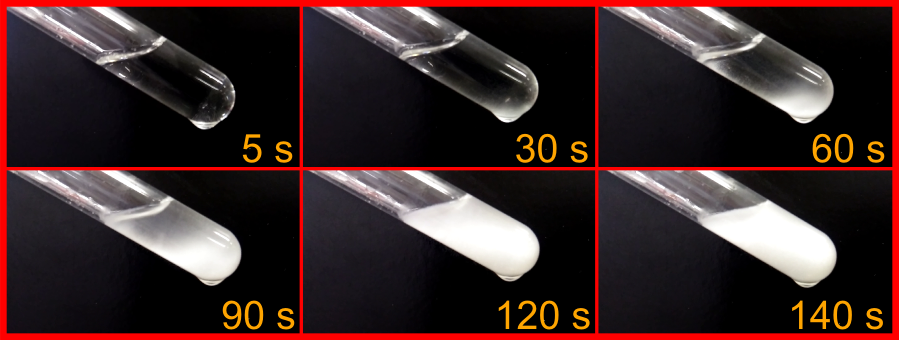
\includegraphics[width=\textwidth]{imagens/ureia/tempos}
	\caption{Resfriamento de uma amostra de \CTAB{} 300 \mM{} e 37\% m/m de ureia. A contagem do tempo se iniciou no instante que a amostra foi removida do banho a 60°C e terminou quando a amostra se mostrou totalmente sólida, e em temperatura ambiente.}
	\label{fig:resfriamento_ureia}
\end{figure} \index{resultados!ureia}


\section{Calorimetria diferencial de varredura (DSC)}
	\index{resultados!\CTAB} \index{resultados!\TTAB} \index{resultados!\DTAB} \index{resultados!DSC} \index{resultados!sem NaSal}
	Foram preparadas soluções de ureia, em várias concentrações, com três surfactantes (\CTAB, \TTAB{} e \DTAB), em nas concentrações de 100, 200 e 300 \mM{} (equivalentes a 3, 6, e 9\% de surfactante, aproximadamente). Os termogramas resultantes foram organizados em figuras de modo a facilitar comparações. A \autoref{tab:refs_DSC} lista as comparações realizadas e em quais figuras estão apresentadas. Essas amostras não possuem memória térmica, então não é necessário realizar uma corrida anterior.
    
    \begin{table}[h]
        \IBGEtab{%
            \caption{Comparações de termogramas de amostras de surfactante (concentração em \mM) e ureia (\% m/m), e suas respectivas figuras}
            \label{tab:refs_DSC}
            }%
            {%
            \begin{tabular}{l p{1.5cm} p{1.5cm}}
                \toprule
    			%\centering
				Surf. e Conc. em \mM             & \% Ureia		 & Figura 			\\
    			\midrule
				\CTAB{} 100	                     & 38---45		 & \ref{fig:DSC_CTAB100_UR38-45}\\
				\CTAB{} 300	                     & 38---45		 & \ref{fig:DSC_CTAB300_UR38-45}\\
				\CTAB{} 100, 200, 300	             & 45, 40	     & \ref{fig:DSC_CTAB_UR40-45}	\\
				\TTAB{} 100, 200, 300	             & 45, 40	     & \ref{fig:DSC_TTAB_UR_40-45}	\\
				\DTAB{} 100, 200, 300	             & 45, 40	     & \ref{fig:DSC_DTAB_UR_40-45}	\\
				% CTAB, TTAB, DTAB 100	         & 45	         & \ref{fig:DSC_Surf_100mm_45p}	\\
				% CTAB, TTAB, DTAB 200	         & 45	         & \ref{fig:DSC_Surf_200mm_45p}	\\
				% CTAB, TTAB, DTAB 300	         & 45	         & \ref{fig:DSC_Surf_300mm_45p}	\\
    			\midrule
				\CTAB{} 100 NaSal 60	             & 35, 40, 45	 & \ref{fig:DSC_NaSal60}		\\
				\CTAB{} 100 NaSal 100	             & 35, 40, 45	 & \ref{fig:DSC_NaSal100}	\\
				\CTAB{} 100 NaSal 250	             & 35, 40, 45	 & \ref{fig:DSC_NaSal250}	\\
				% CTAB 100 NaSal 60, 100, 250    & 35 	         & \ref{fig:DSC_NaSal_Ur35}  \\
				% CTAB 100 NaSal 60, 100, 250    & 40	             & \ref{fig:DSC_NaSal_Ur40}  \\
				% CTAB 100 NaSal 60, 100, 250	 & 45	         & \ref{fig:DSC_NaSal_Ur45}  \\
    			\bottomrule
            \end{tabular}%
            }{}
    \end{table}
	

%	\begin{figure}[H]
%		\centering
%		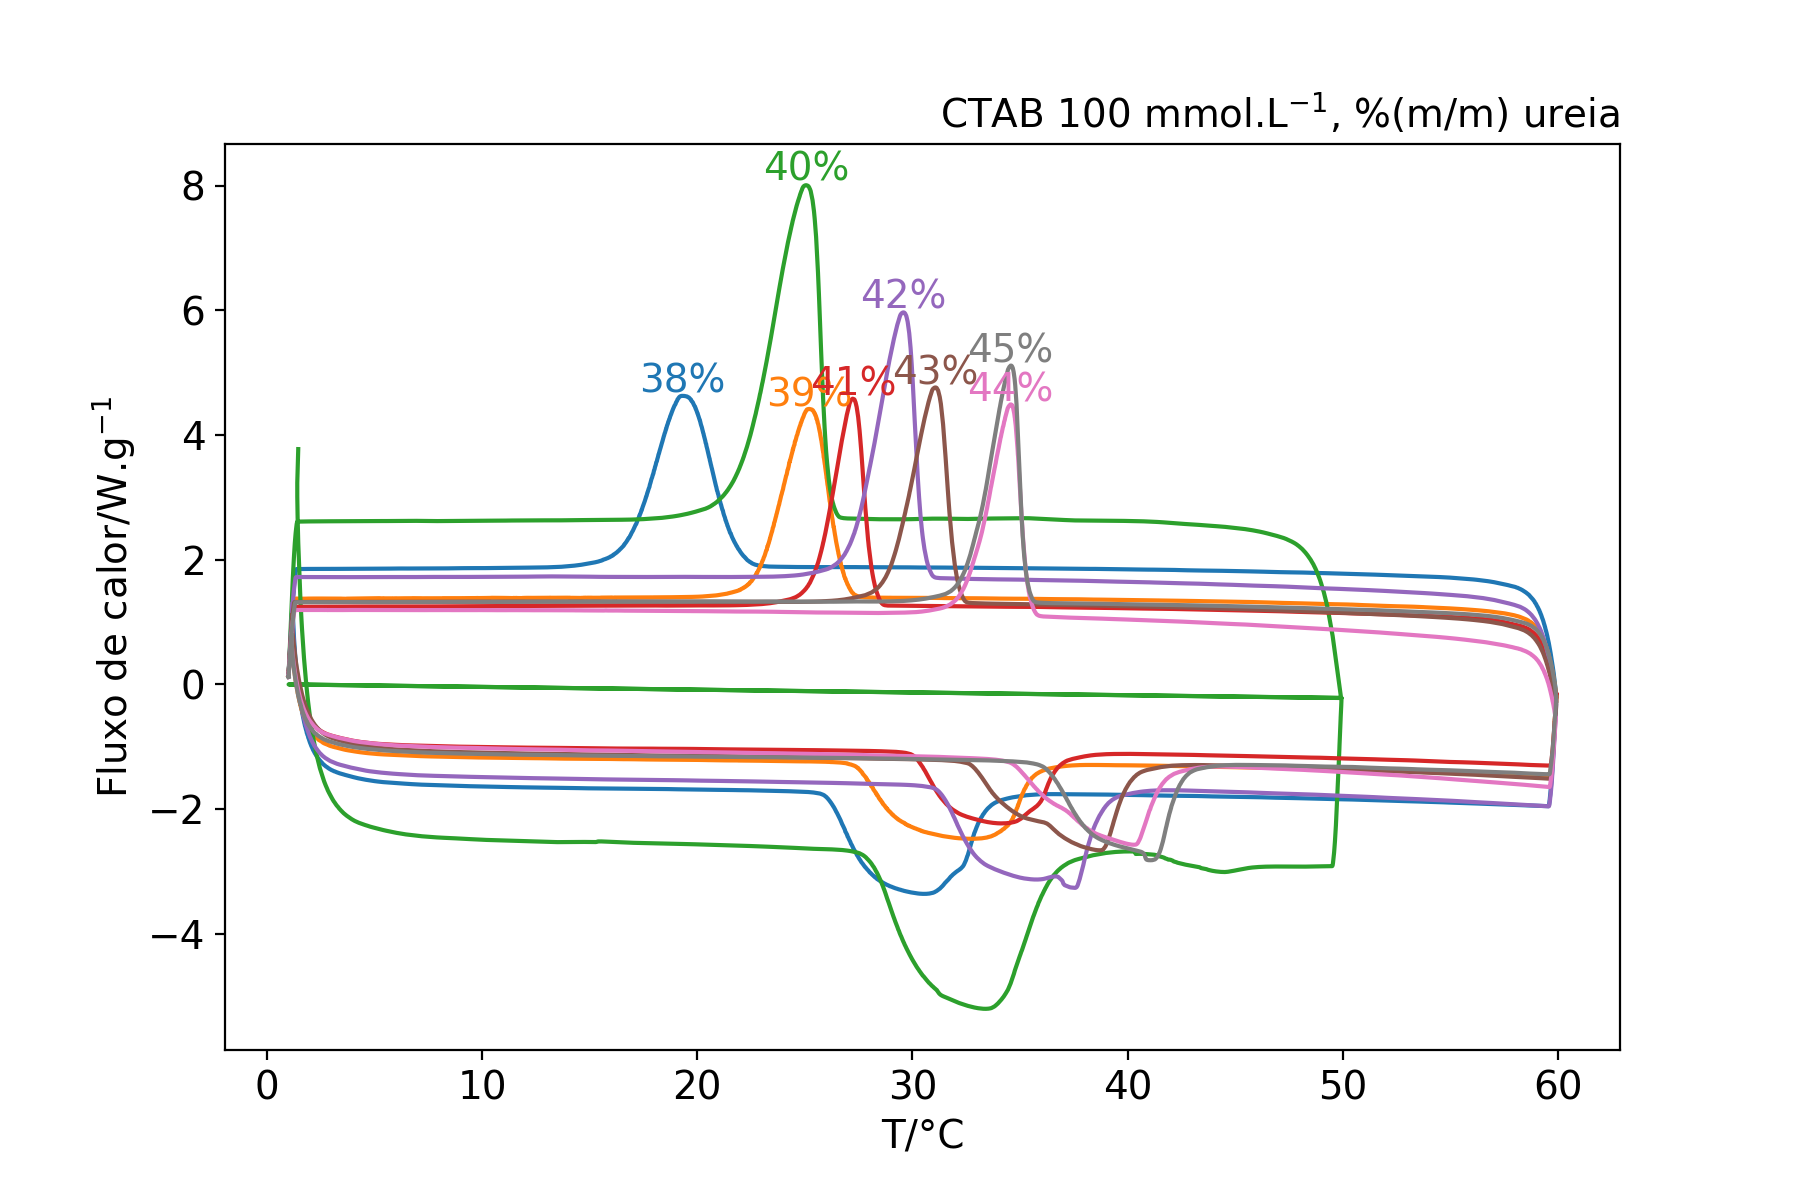
\includegraphics[width=0.75\textwidth]{./imagens/dsc/CTAB_porc_ur}
%		\caption{Termogramas de soluções de CTAB 100 \mM{} em concentrações crescentes de ureia, de 38\% m/m a 45\% m/m}
%		\label{fig:DSC_CTAB_UR38-45}
%	\end{figure}

	\begin{figure}[h]
		\begin{subfigure}[t]{0.5\textwidth}
			\centering
			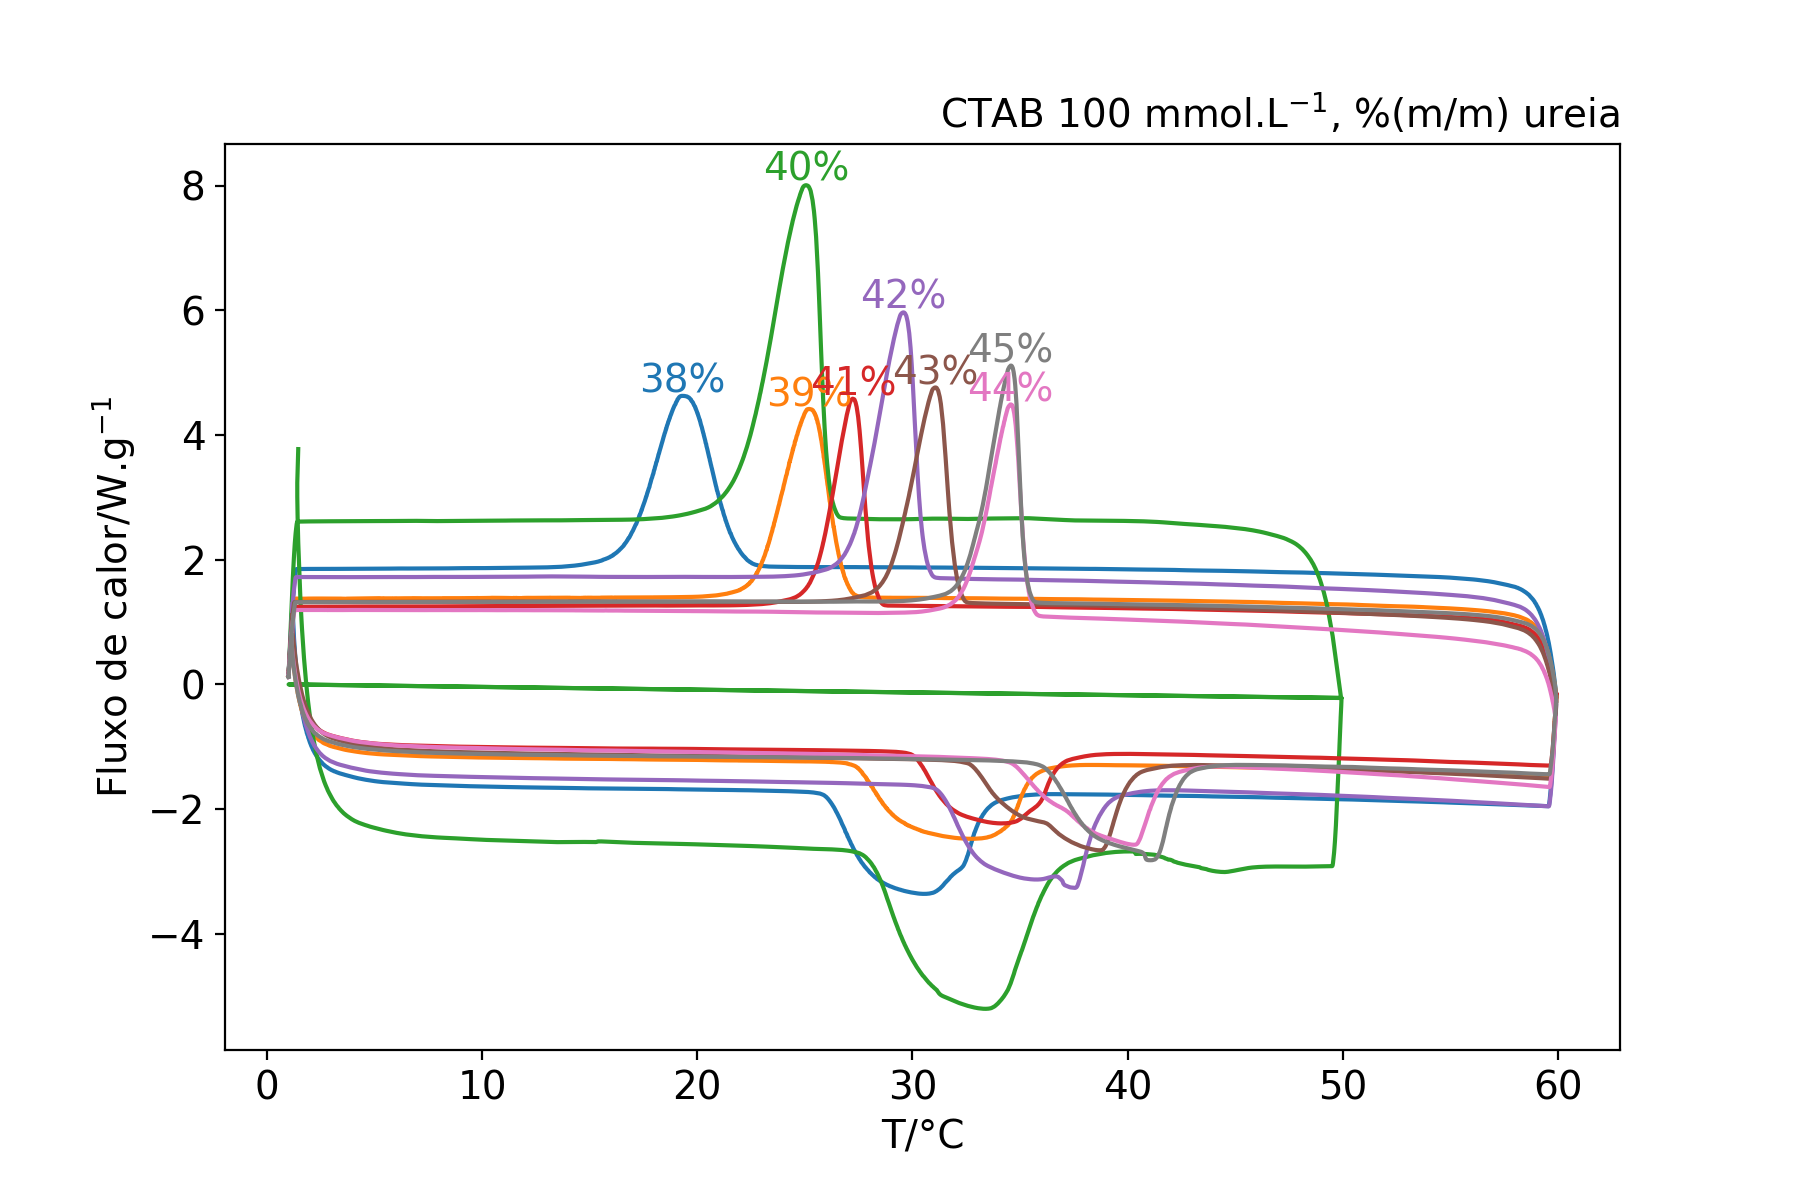
\includegraphics[width=\textwidth]{./imagens/dsc/CTAB_porc_ur}
			\caption{\CTAB{} 100 \mM{}}
			\label{fig:DSC_CTAB100_UR38-45}	
		\end{subfigure}%
		\begin{subfigure}[t]{0.5\textwidth}
			\centering
			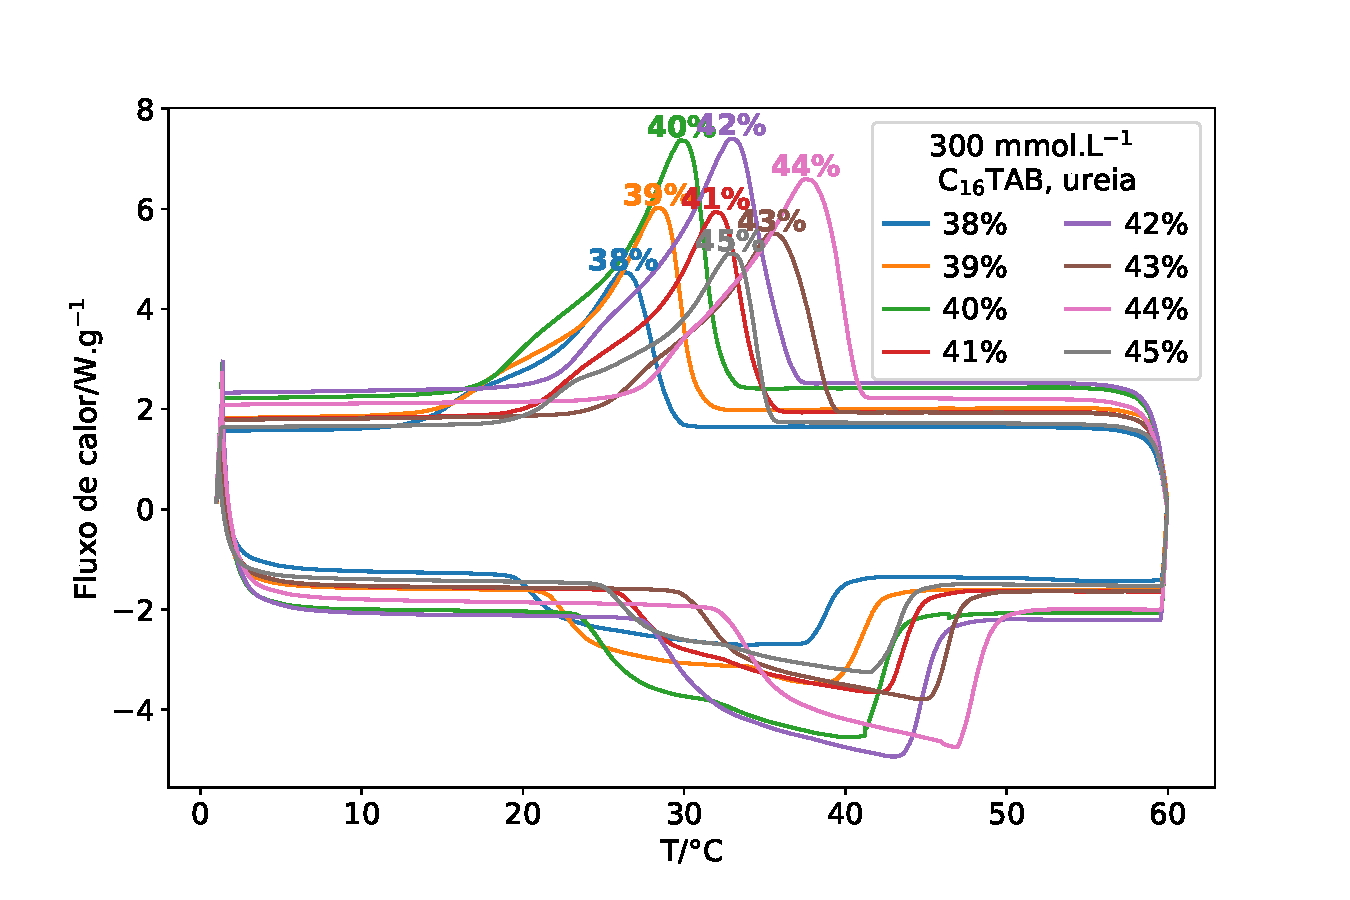
\includegraphics[width=\textwidth]{./imagens/dsc/CTAB_300_porc_ur}
			\caption{\CTAB{} 300 \mM}
			\label{fig:DSC_CTAB300_UR38-45}
		\end{subfigure}
		\caption{Termogramas de soluções de \CTAB{} 100 \mM{} (\ref{fig:DSC_CTAB100_UR38-45}) e 300 \mM{} (\ref{fig:DSC_CTAB300_UR38-45}), em concentrações crescentes de ureia, de 38 a 45\% m/m.}
		\label{fig:DSC_CTAB_100_300_Ur38-45}
	\end{figure}
	
	\begin{figure}[h]
		\begin{subfigure}[t]{0.5\textwidth}
			\centering
			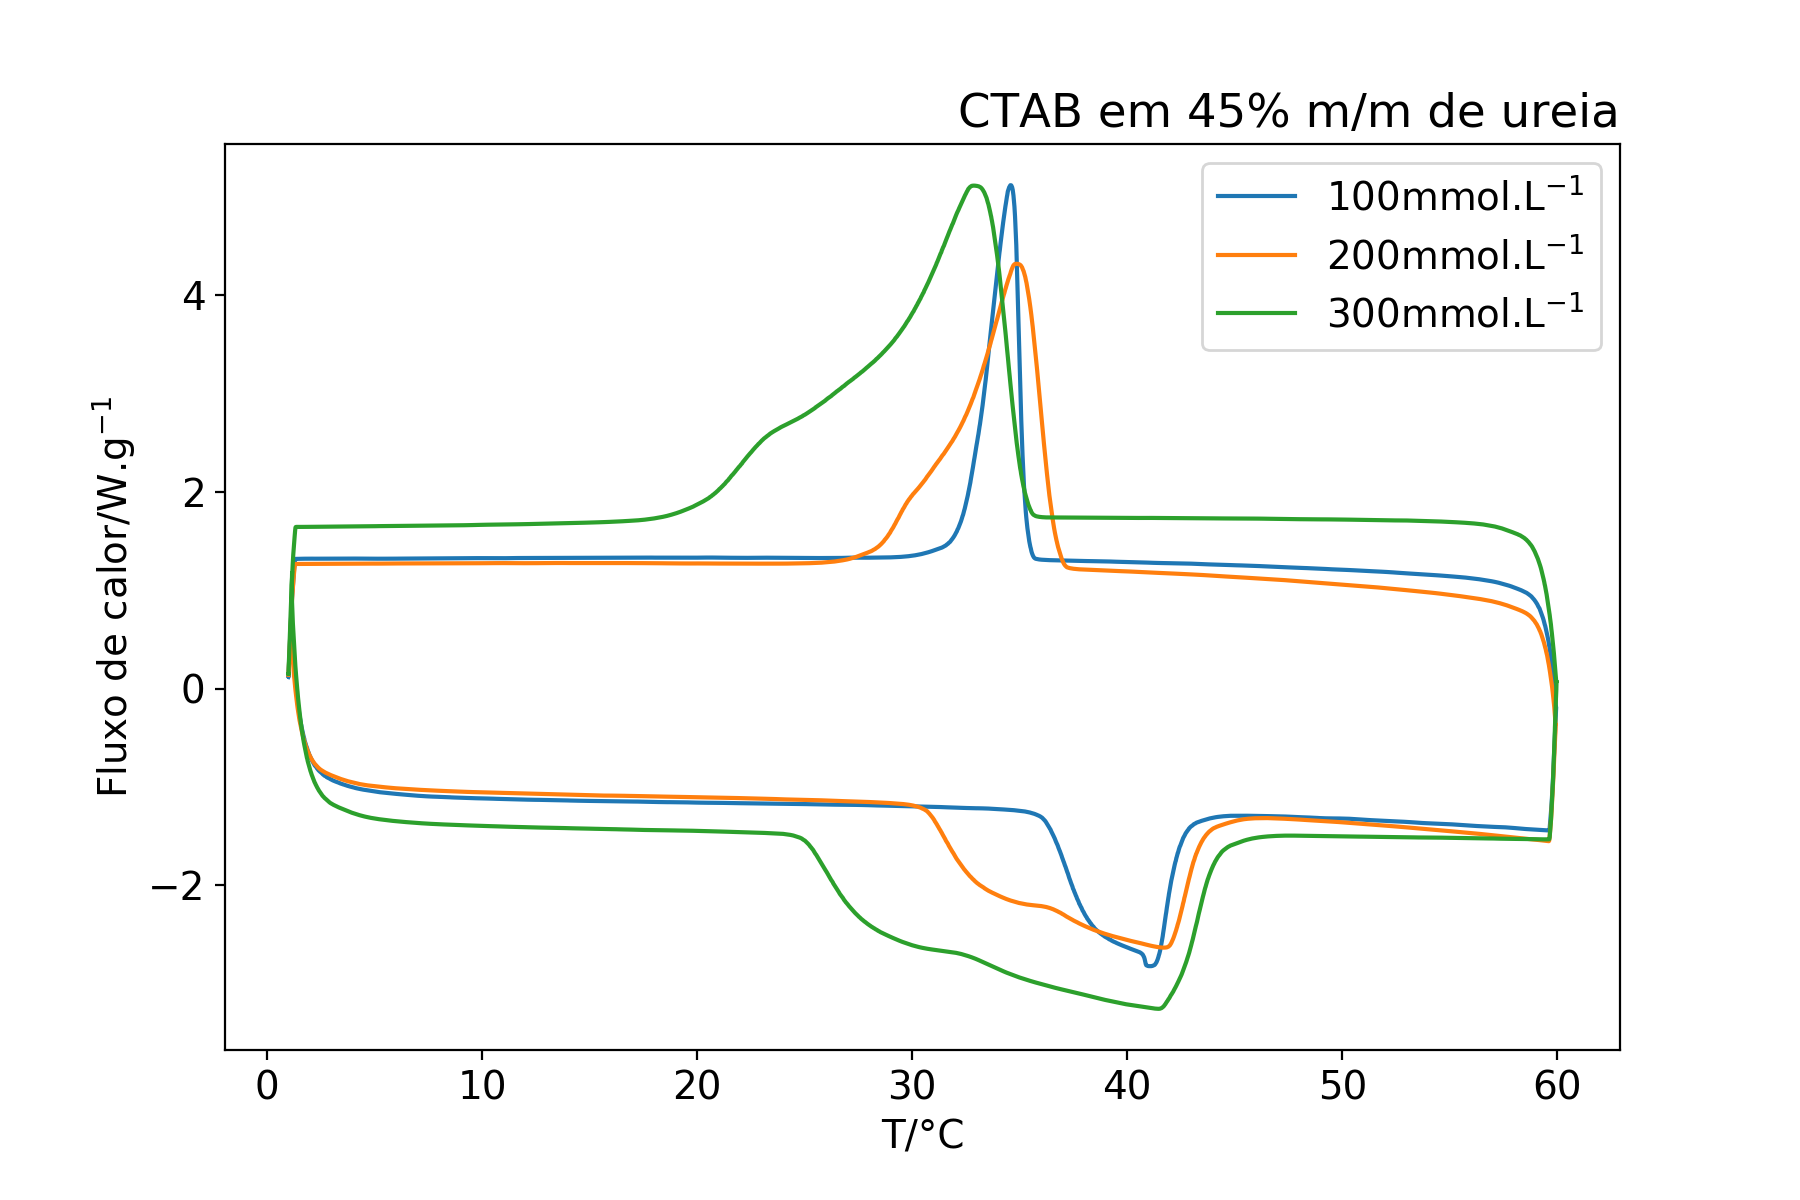
\includegraphics[width=\textwidth]{./imagens/dsc/CTAB_45p}
			\caption{45\% de ureia}
			\label{fig:DSC_CTAB_UR45}
		\end{subfigure}  %
		\begin{subfigure}[t]{0.5\textwidth}
			\centering
			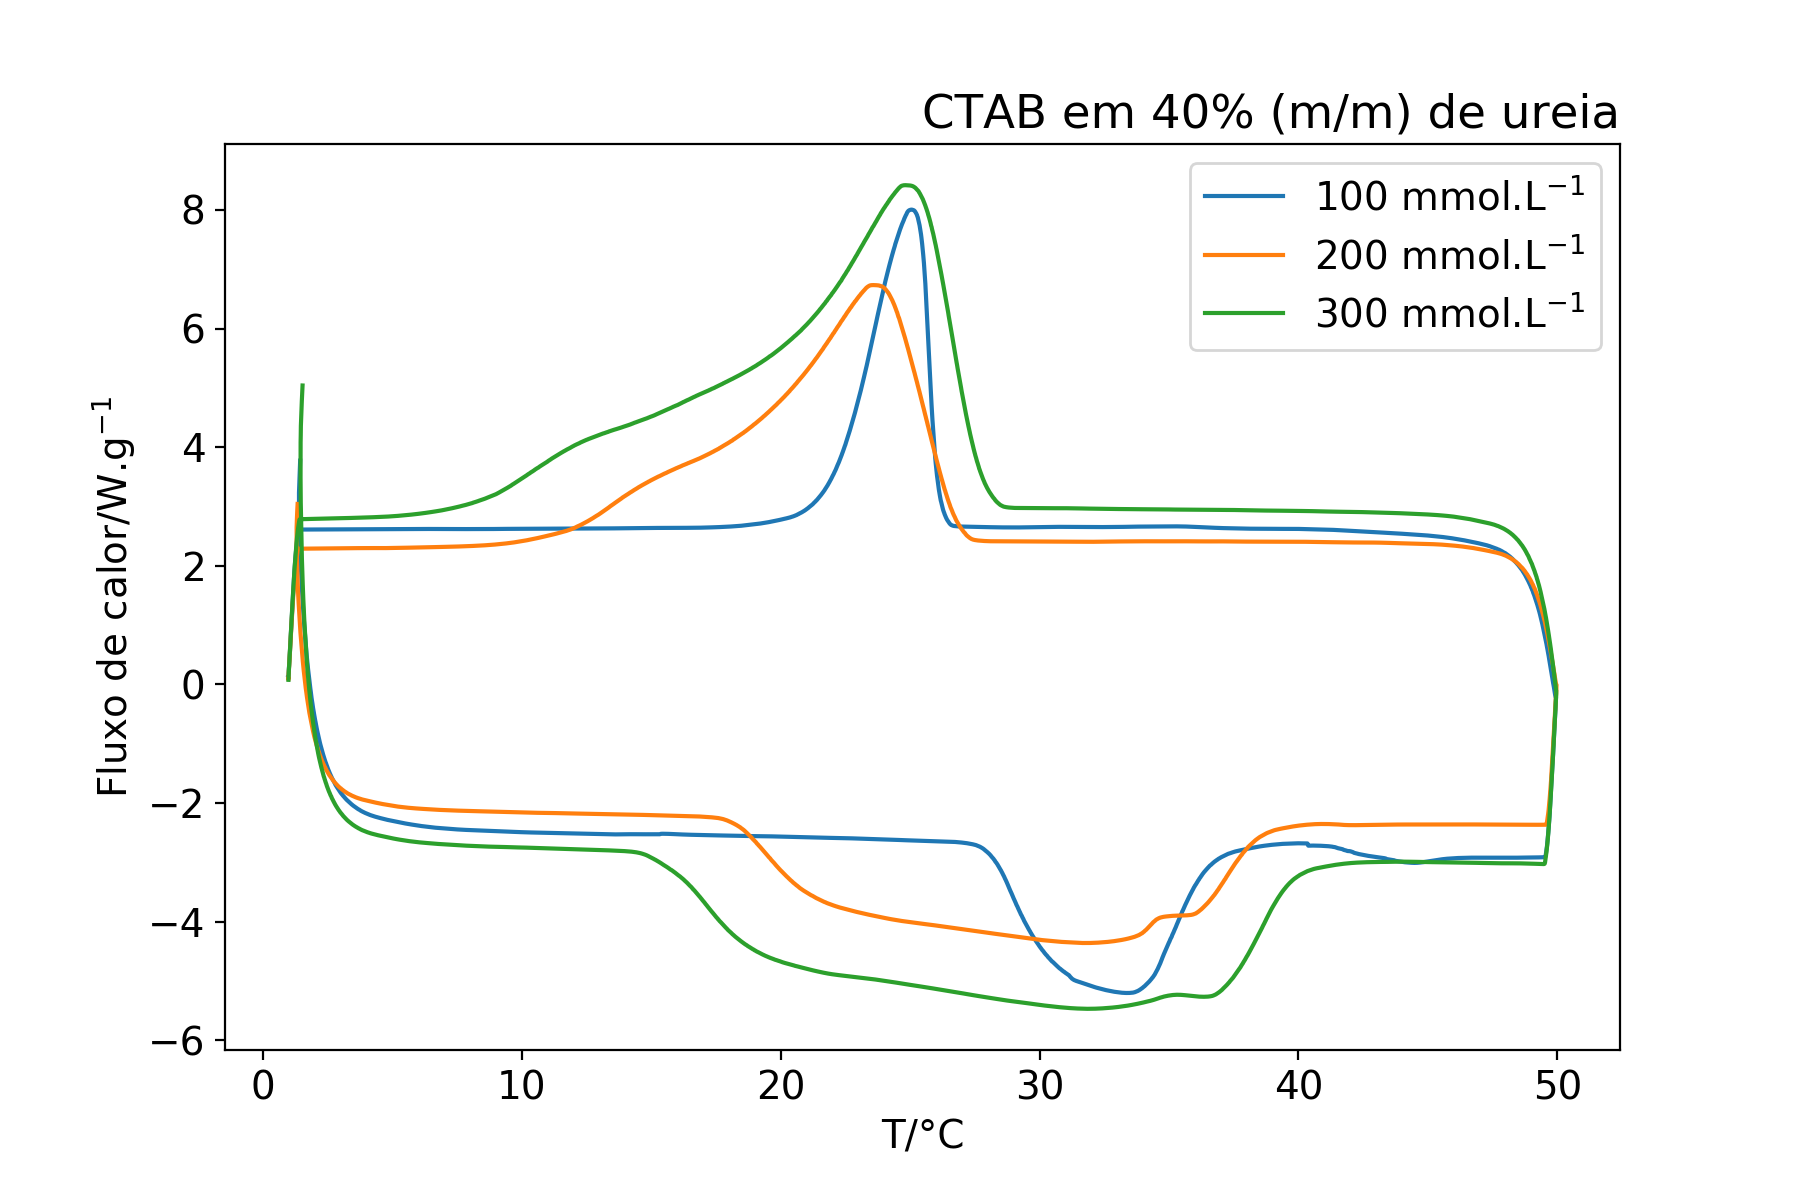
\includegraphics[width=\textwidth]{./imagens/dsc/CTAB_40p}
			\caption{40\% de ureia}
			\label{fig:DSC_CTAB_UR40}
		\end{subfigure}
		\caption{Termogramas de \CTAB{} 100, 200 e 300 \mM{} em soluções em 45\% (\ref{fig:DSC_CTAB_UR45}) e 40\% (\ref{fig:DSC_CTAB_UR40})}
		\label{fig:DSC_CTAB_UR40-45}
	\end{figure}

	\begin{figure}[h]
		\begin{subfigure}[t]{0.5\textwidth}
			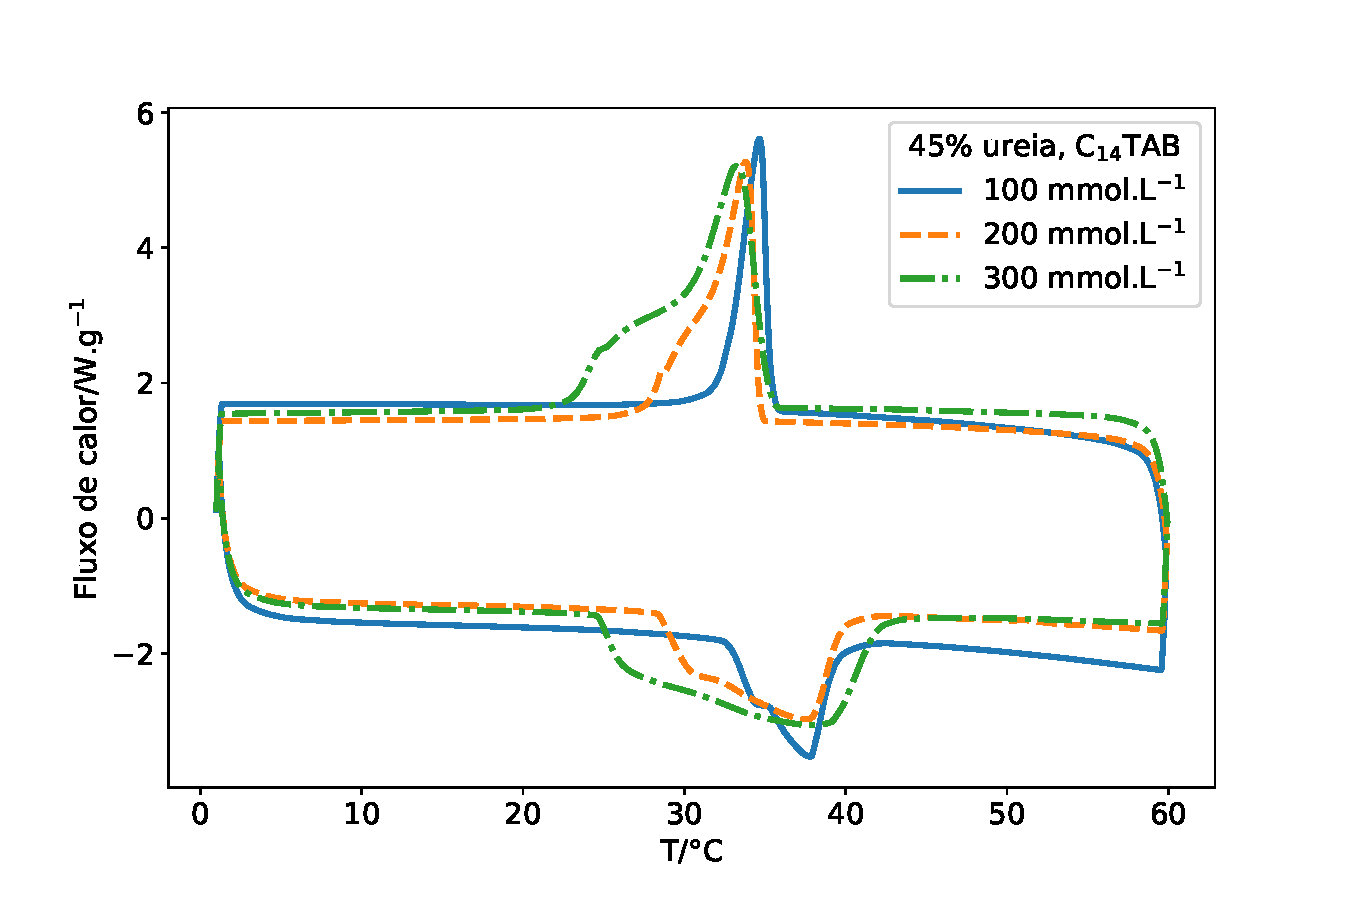
\includegraphics[width=\textwidth]{./imagens/dsc/TTAB_45p}
			\caption{45\% de ureia}
			\label{fig:DSC_TTAB_UR45}
		\end{subfigure}%
		\begin{subfigure}[t]{0.5\textwidth}
			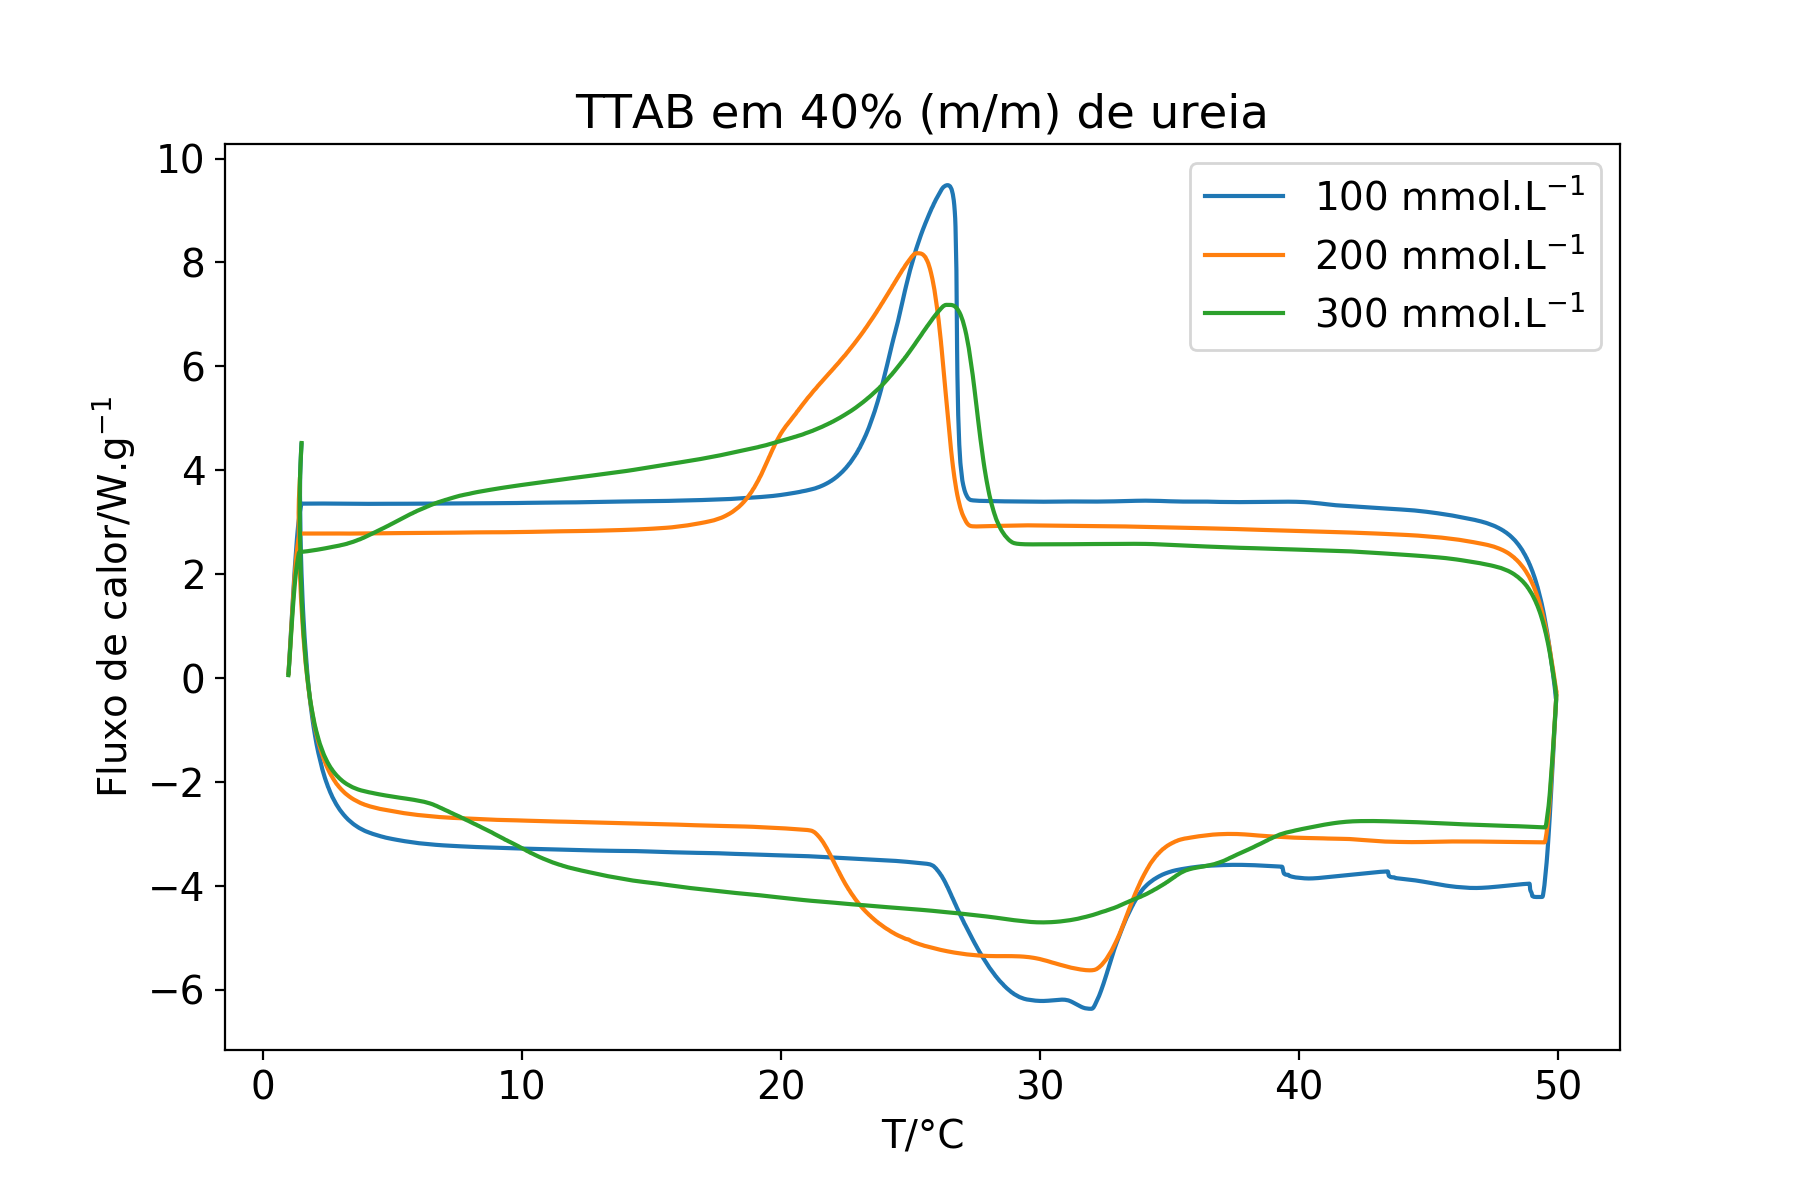
\includegraphics[width=\textwidth]{./imagens/dsc/TTAB_40p}
			\caption{40\% de ureia}
			\label{fig:DSC_TTAB_UR40}
		\end{subfigure}
		\caption{Termogramas de soluções de \TTAB{} 100, 200 e 300 \mM{}, em 45\% (\ref{fig:DSC_TTAB_UR45}) e 40\% (\ref{fig:DSC_TTAB_UR40}) de ureia}
		\label{fig:DSC_TTAB_UR_40-45}
	\end{figure}
	
	\begin{figure}[h]
		\begin{subfigure}[t]{0.5\textwidth}
			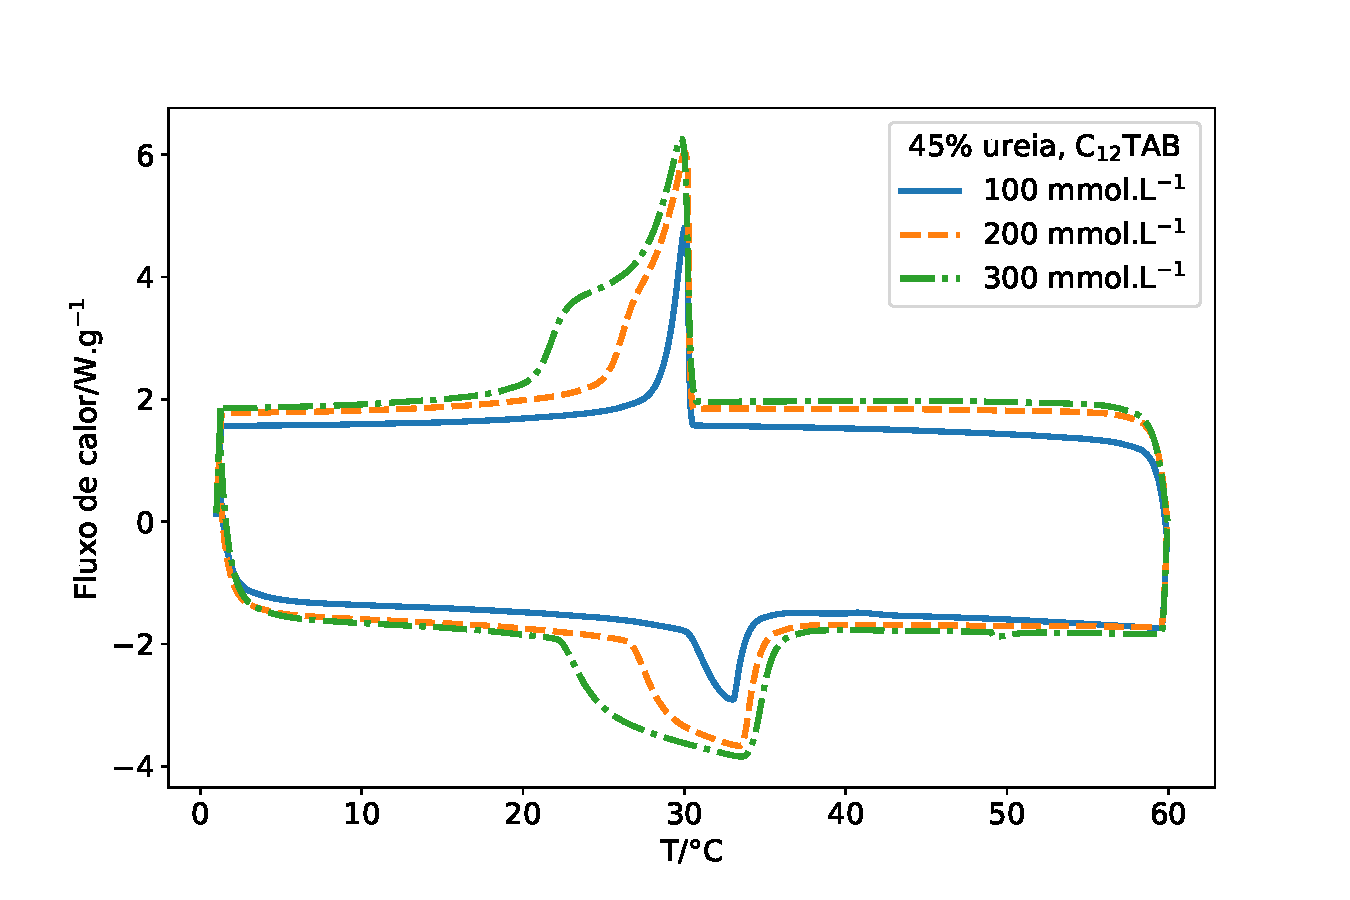
\includegraphics[width=\textwidth]{./imagens/dsc/DTAB_45p}
			\caption{45\% de ureia}
			\label{fig:DSC_DTAB_UR45}
		\end{subfigure}%
		\begin{subfigure}[t]{0.5\textwidth}
			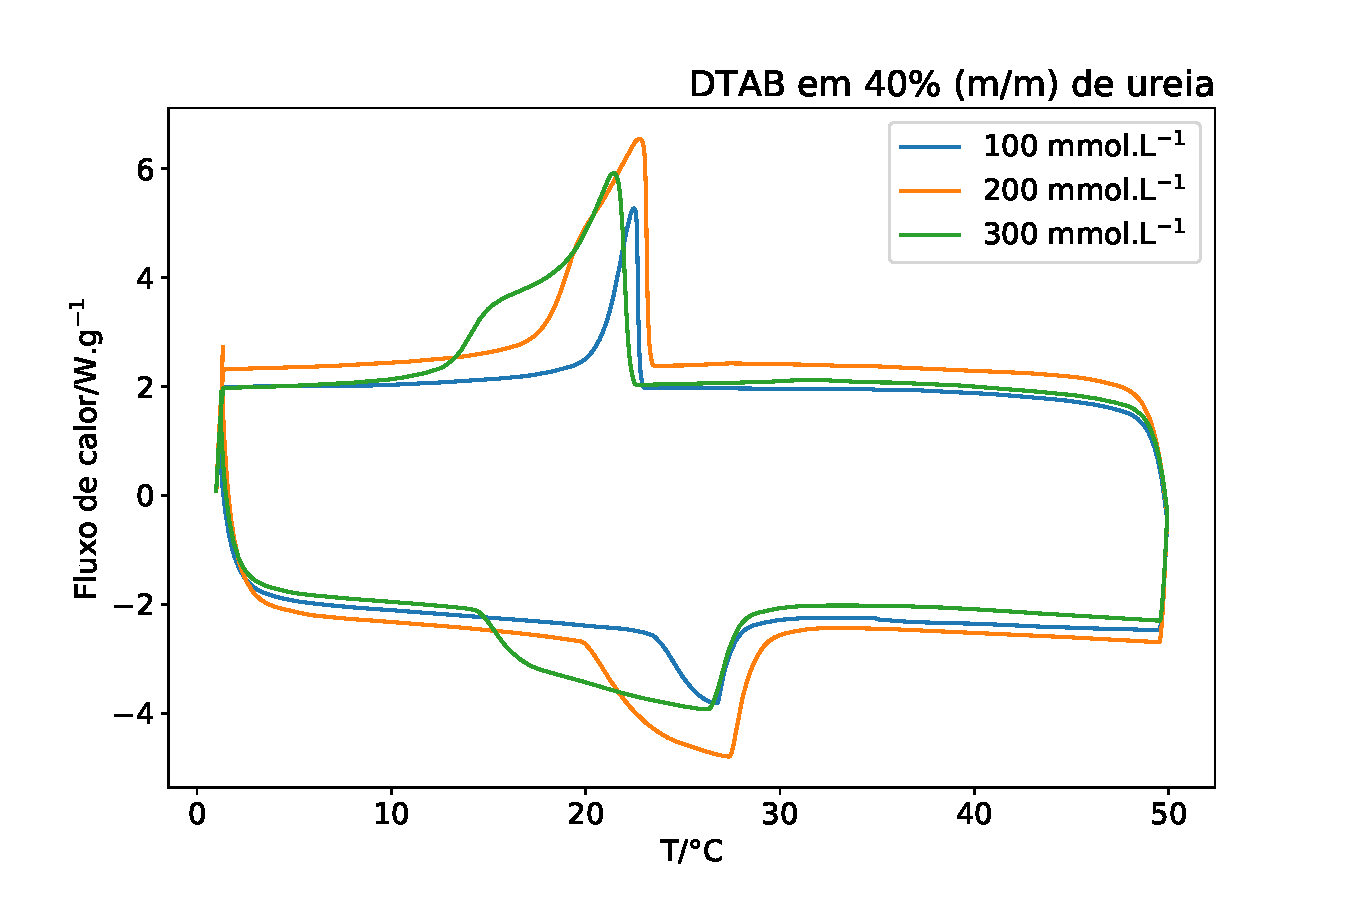
\includegraphics[width=\textwidth]{./imagens/dsc/DTAB_40p}
			\caption{40\% de ureia}
			\label{fig:DSC_DTAB_UR40}
		\end{subfigure}
		\caption{Termogramas de soluções de \DTAB{} 100, 200 e 300 \mM{}, em 45\% (\ref{fig:DSC_DTAB_UR45}) e 40\% (\ref{fig:DSC_DTAB_UR40}) de ureia}
		\label{fig:DSC_DTAB_UR_40-45}
	\end{figure}
	
%		
%		% todo: verificar se a notação (C|T|D) é boa
%		\begin{figure}[H]
%			\centering
%			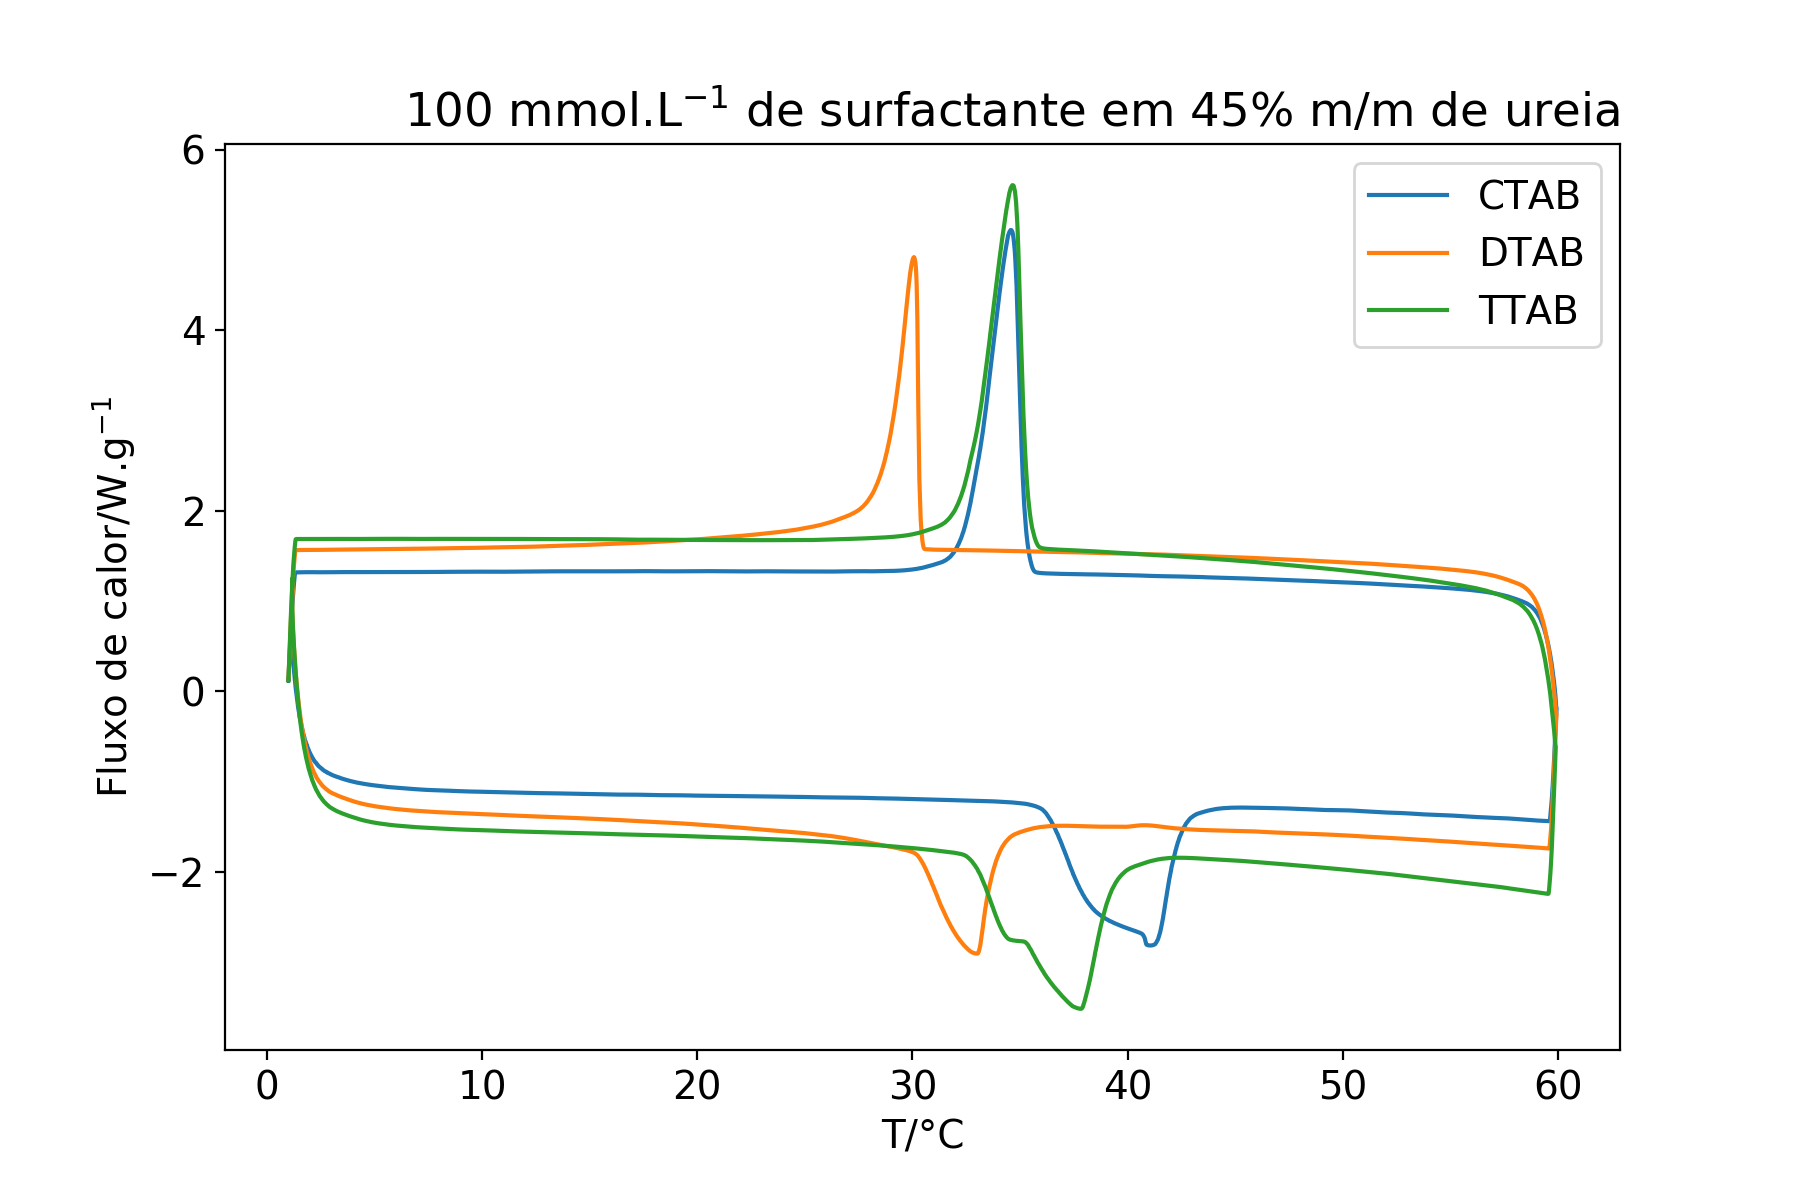
\includegraphics[width=0.60\textwidth]{./imagens/dsc/Surf_100mm_45p}
%			\caption{Termogramas de soluções de (C|T|D)TAB 100 \mM{}, em 45\% de ureia}
%			\label{fig:DSC_Surf_100mm_45p}
%		\end{figure}
%	
%		\begin{figure}[H]
%			\centering
%			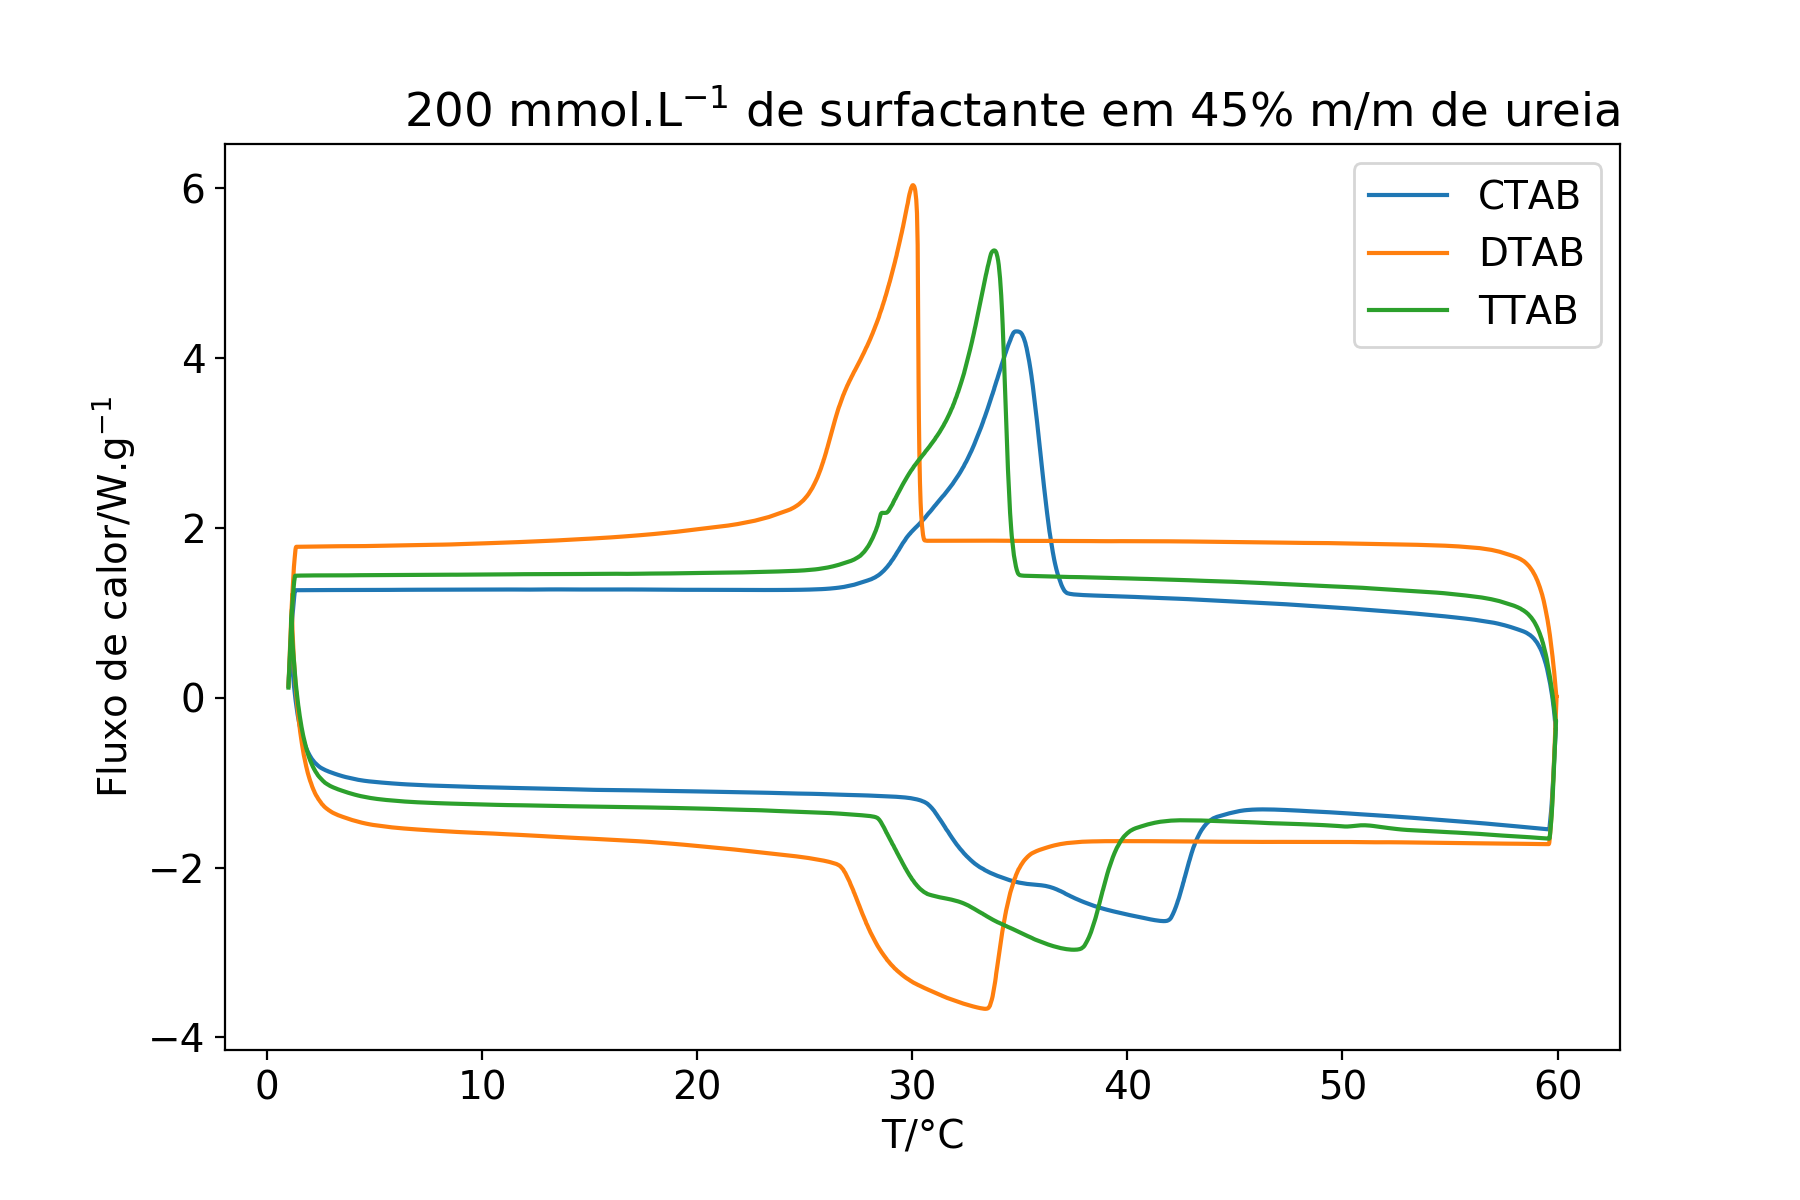
\includegraphics[width=0.60\textwidth]{./imagens/dsc/Surf_200mm_45p}
%			\caption{Termogramas de soluções de (C|T|D)TAB 200 \mM{}, em 45\% de ureia}
%			\label{fig:DSC_Surf_200mm_45p}
%		\end{figure}
%	
%		\begin{figure}[H]
%			\centering
%			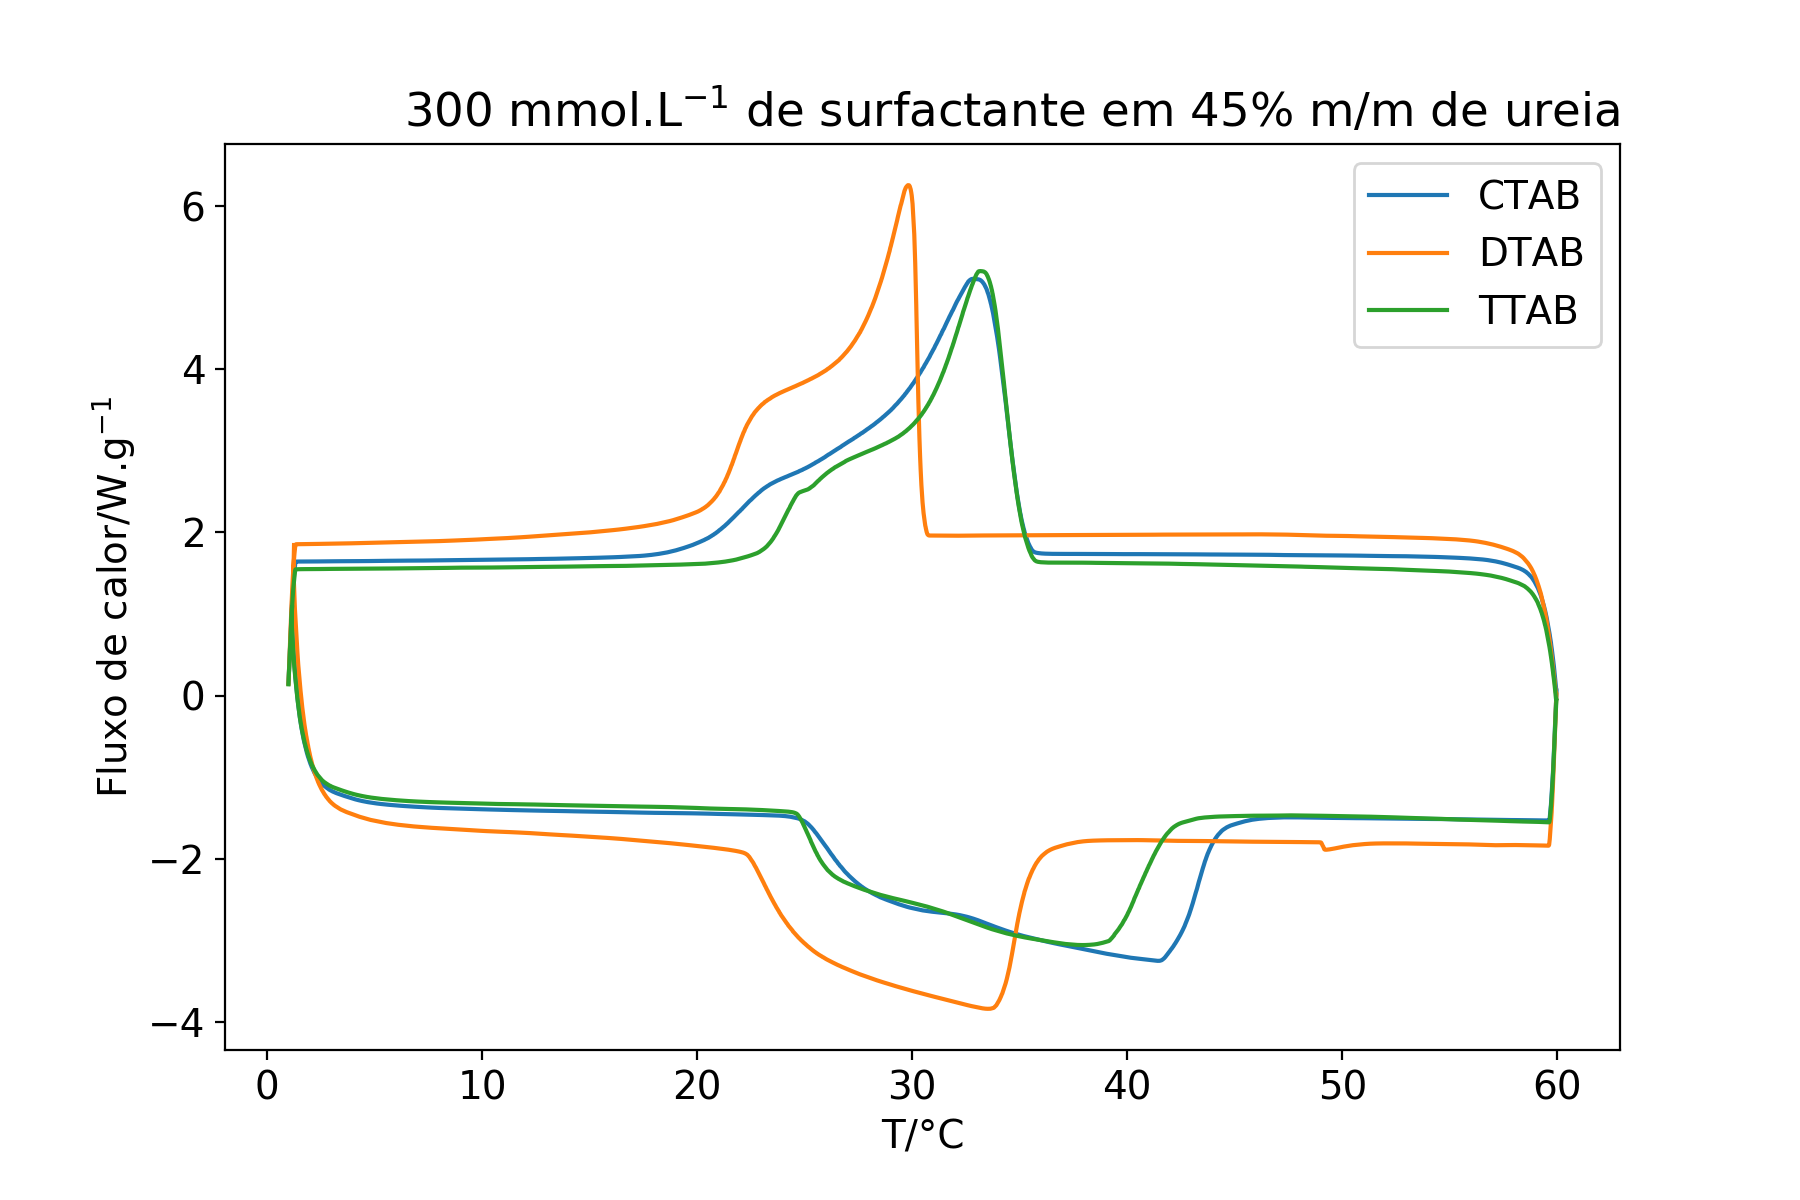
\includegraphics[width=0.60\textwidth]{./imagens/dsc/Surf_300mm_45p}
%			\caption{Termogramas de soluções de (C|T|D)TAB 300 \mM{}, em 45\% de ureia}
%			\label{fig:DSC_Surf_300mm_45p}
%		\end{figure}

\begin{figure}
	\begin{subfigure}{0.5\textwidth}
		\centering
		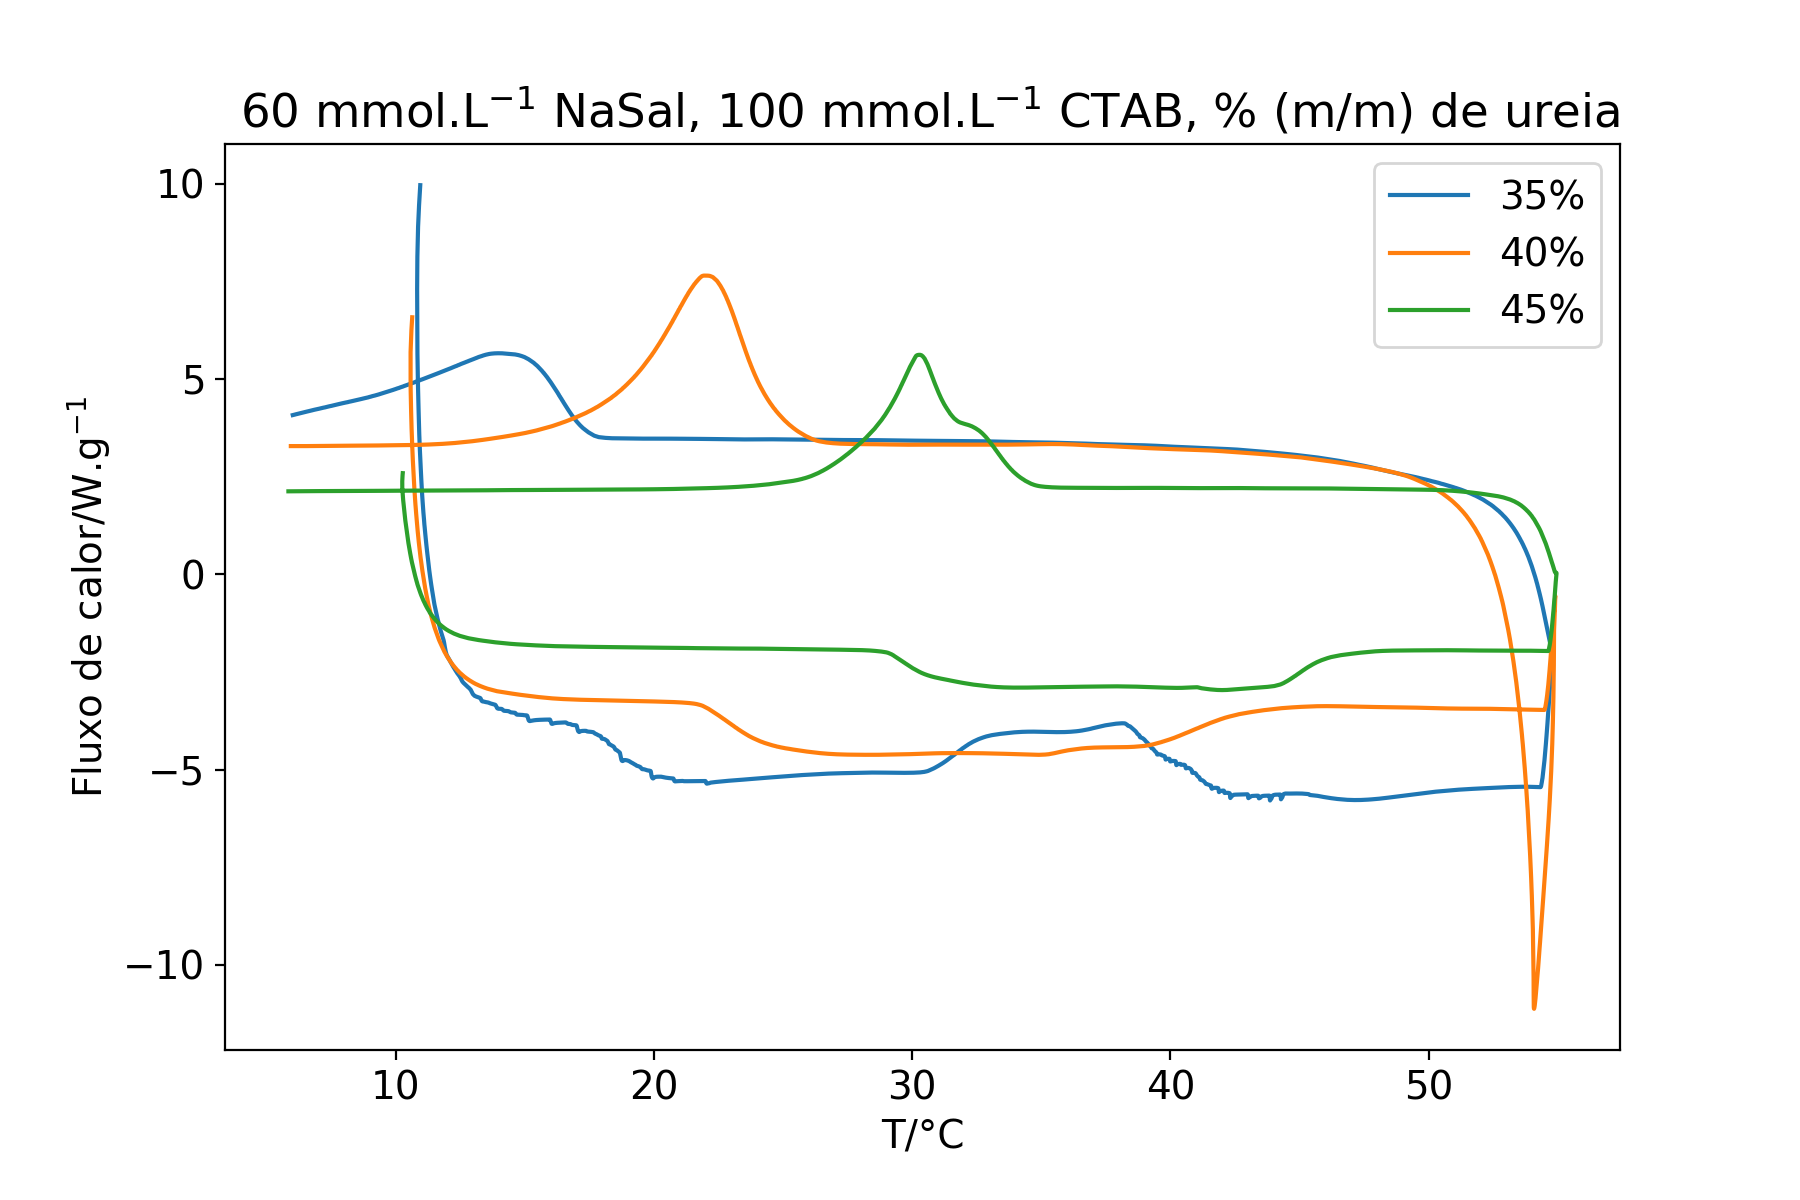
\includegraphics[width=\textwidth]{./imagens/dsc/NaSal60}
		\caption{NaSal 60 \mM}
		\label{fig:DSC_NaSal60}
	\end{subfigure}  %
	\begin{subfigure}{0.5\textwidth}
		\centering
		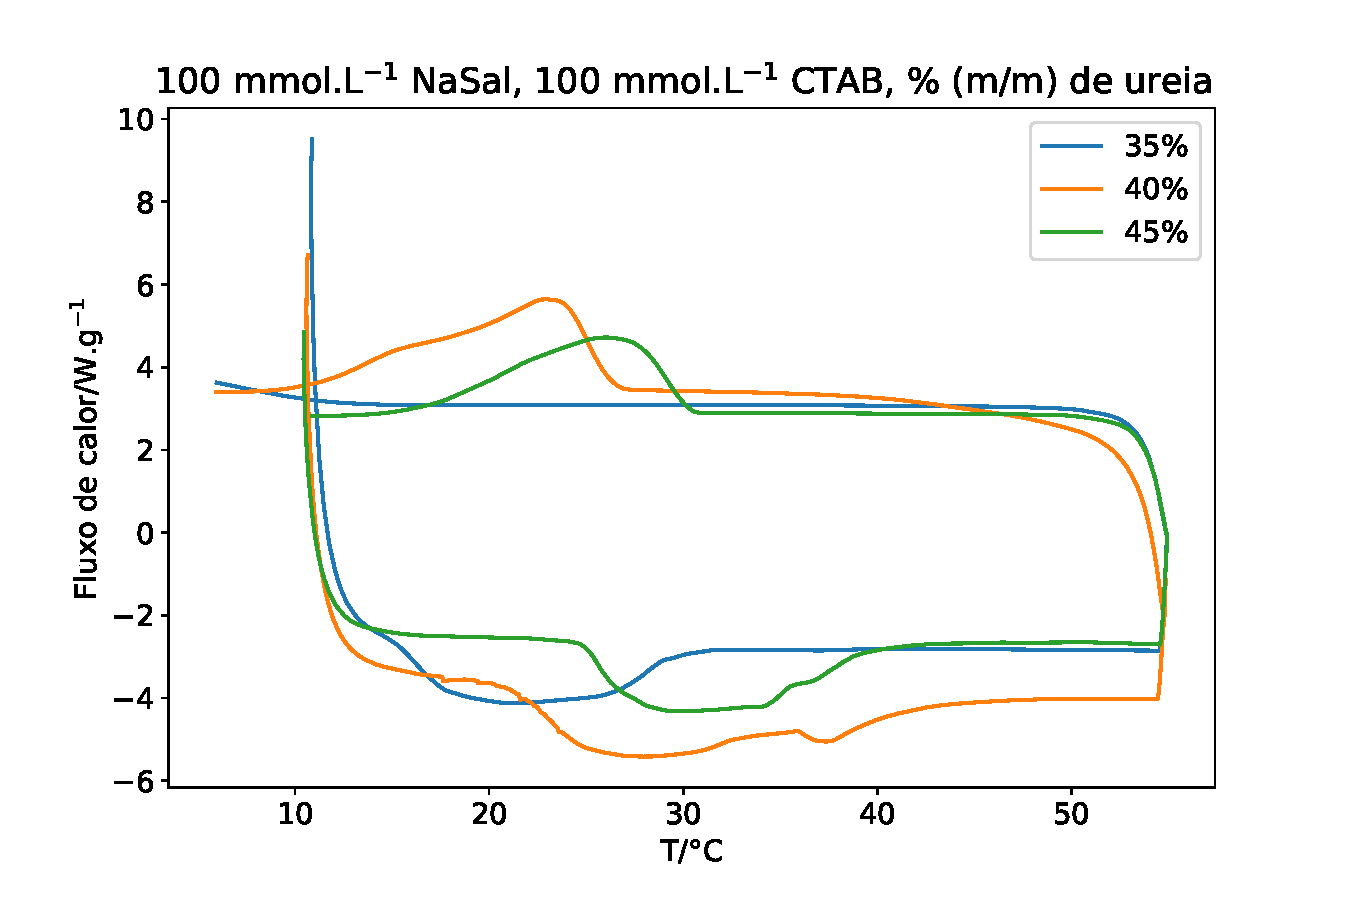
\includegraphics[width=\textwidth]{./imagens/dsc/NaSal100}
		\caption{NaSal 100 \mM}
		\label{fig:DSC_NaSal100}
	\end{subfigure}
	
	\hspace{4cm} \begin{subfigure}{0.5\textwidth}
		\centering
		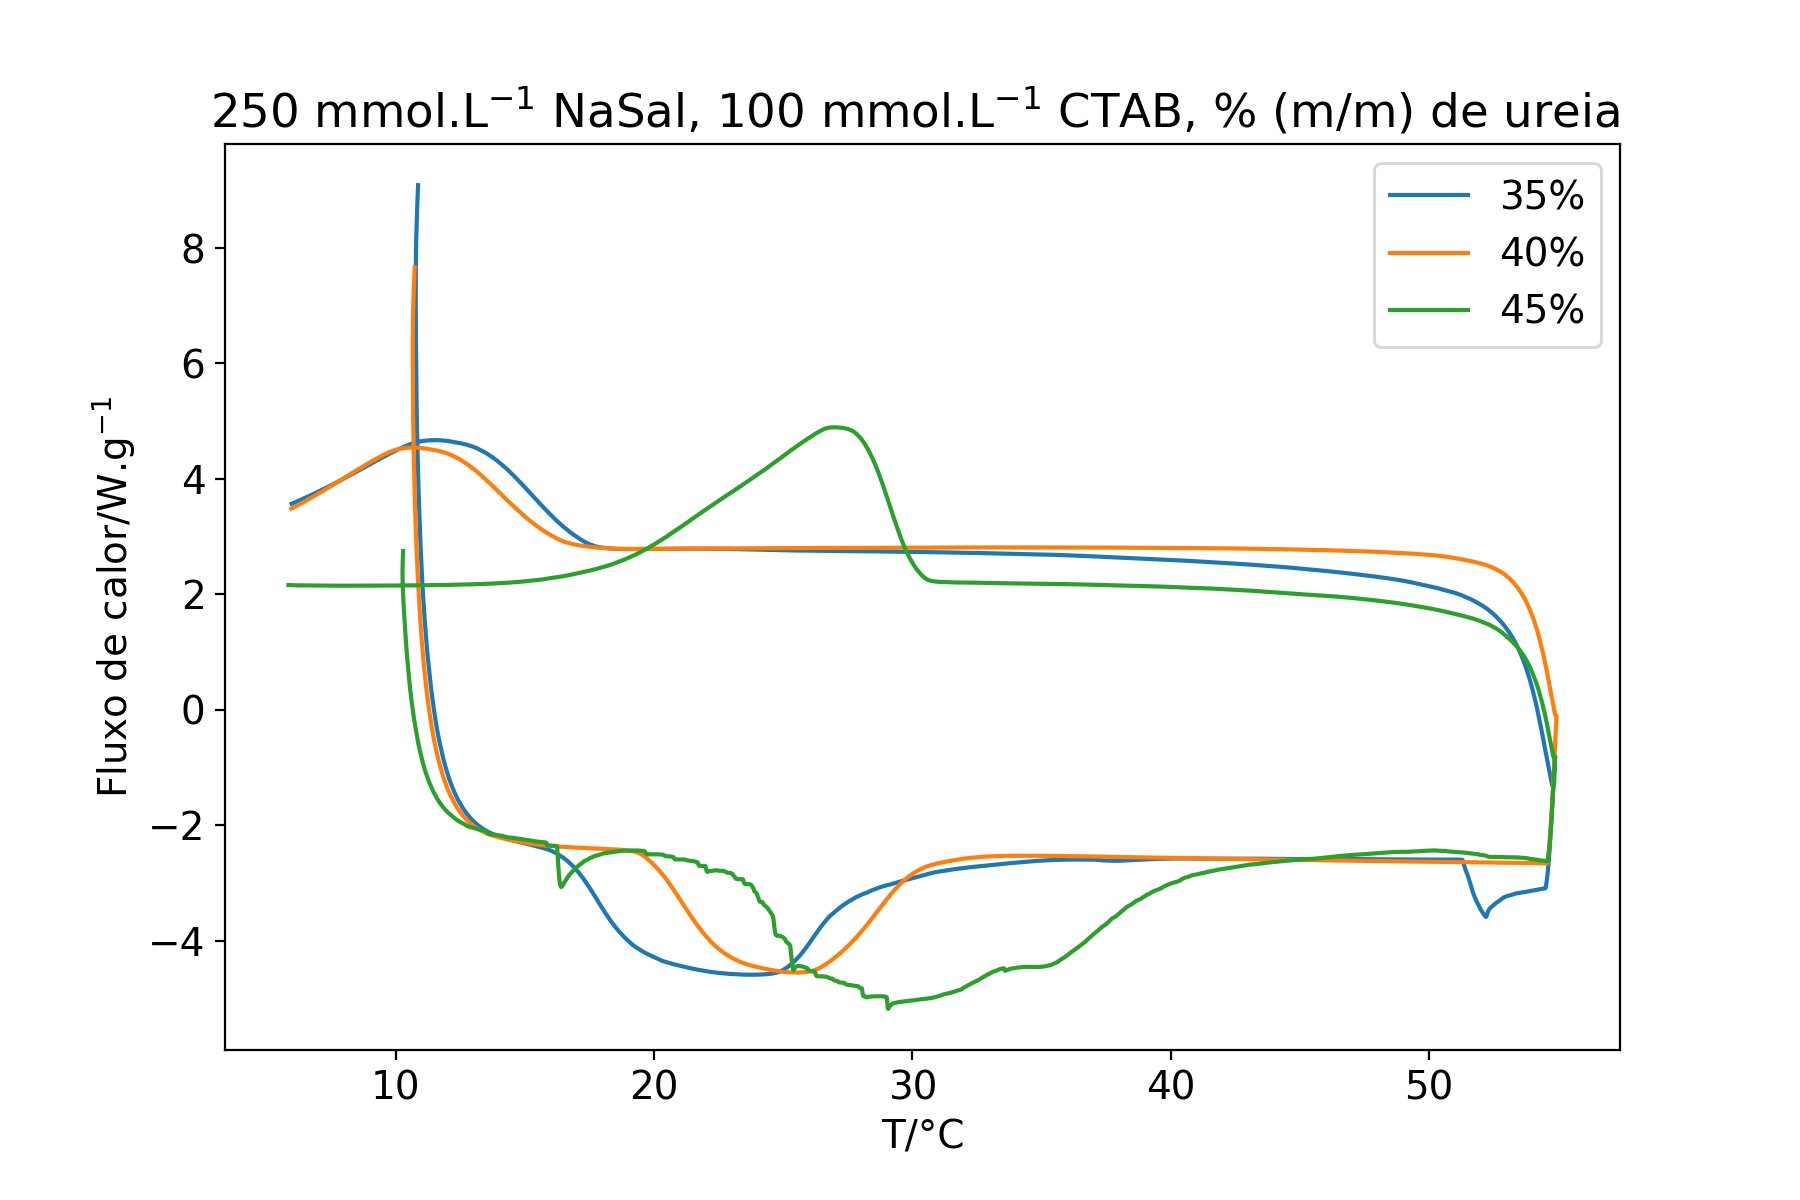
\includegraphics[width=\textwidth]{./imagens/dsc/NaSal250}
		\caption{NaSal 250 \mM}
		\label{fig:DSC_NaSal250}
	\end{subfigure}

	\caption{Termogramas de soluções de NaSal 60, 100 e 250 \mM{} e \CTAB{} 100 \mM{}, em 35\%, 40\% e 45\% (m/m) de ureia}
	\label{fig:DSC_NaSals}  % todo: se isso for ficar numa página só, aumentar o tamanho dos gráficos e colocar para caber

\end{figure}

%	
%		\begin{figure}[H]
%			\centering
%			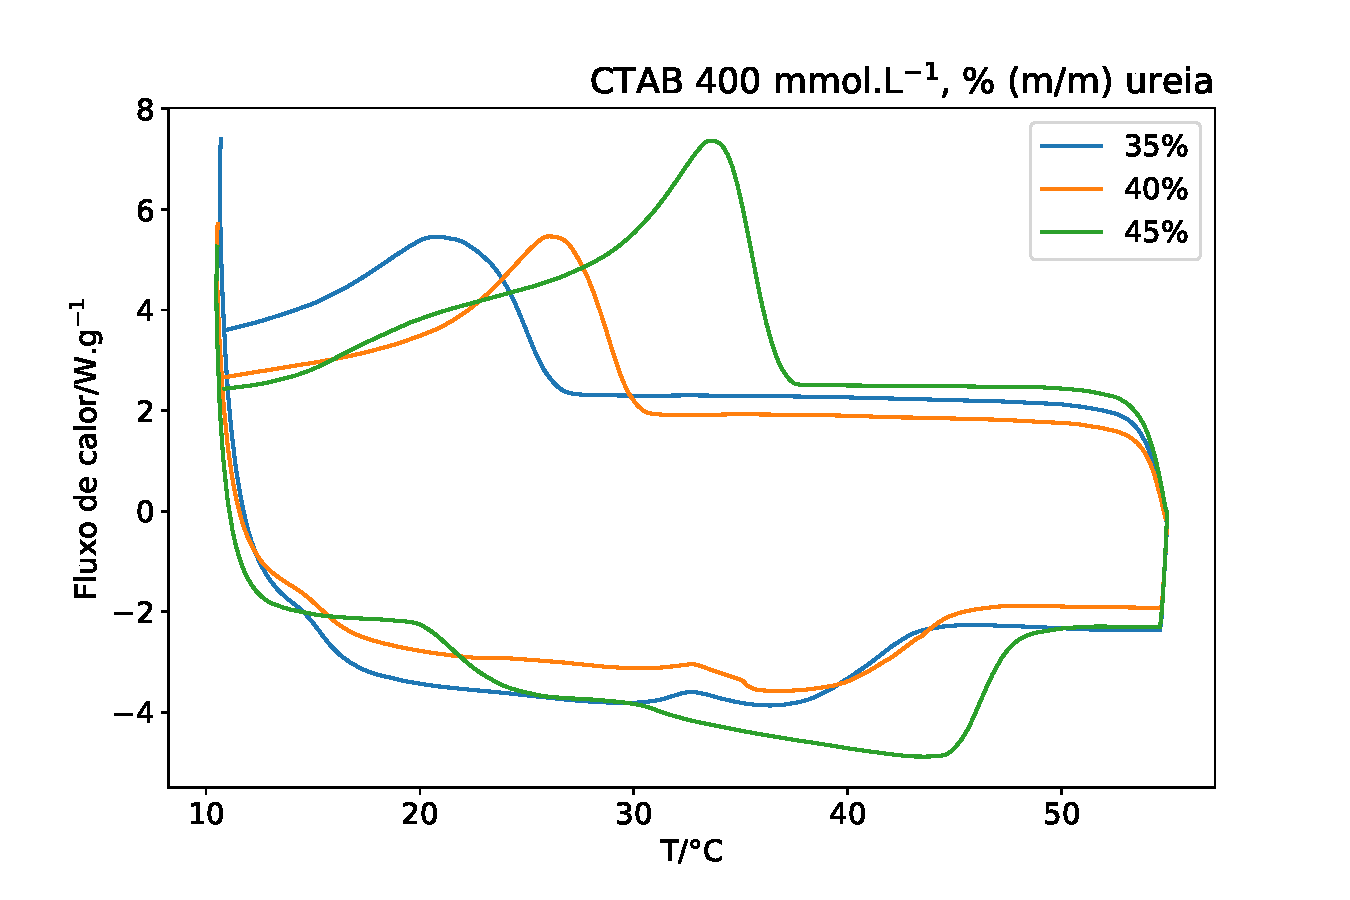
\includegraphics[width=0.60\textwidth]{./imagens/dsc/NaSal35}
%			\caption{Termogramas de soluções de NaSal 60, 100 e 250\mM{} e CTAB 100 \mM{}, em 35\% (m/m) de ureia}
%			\label{fig:DSC_NaSal_Ur35}
%		\end{figure}
%	
%		\begin{figure}[H]
%			\centering
%			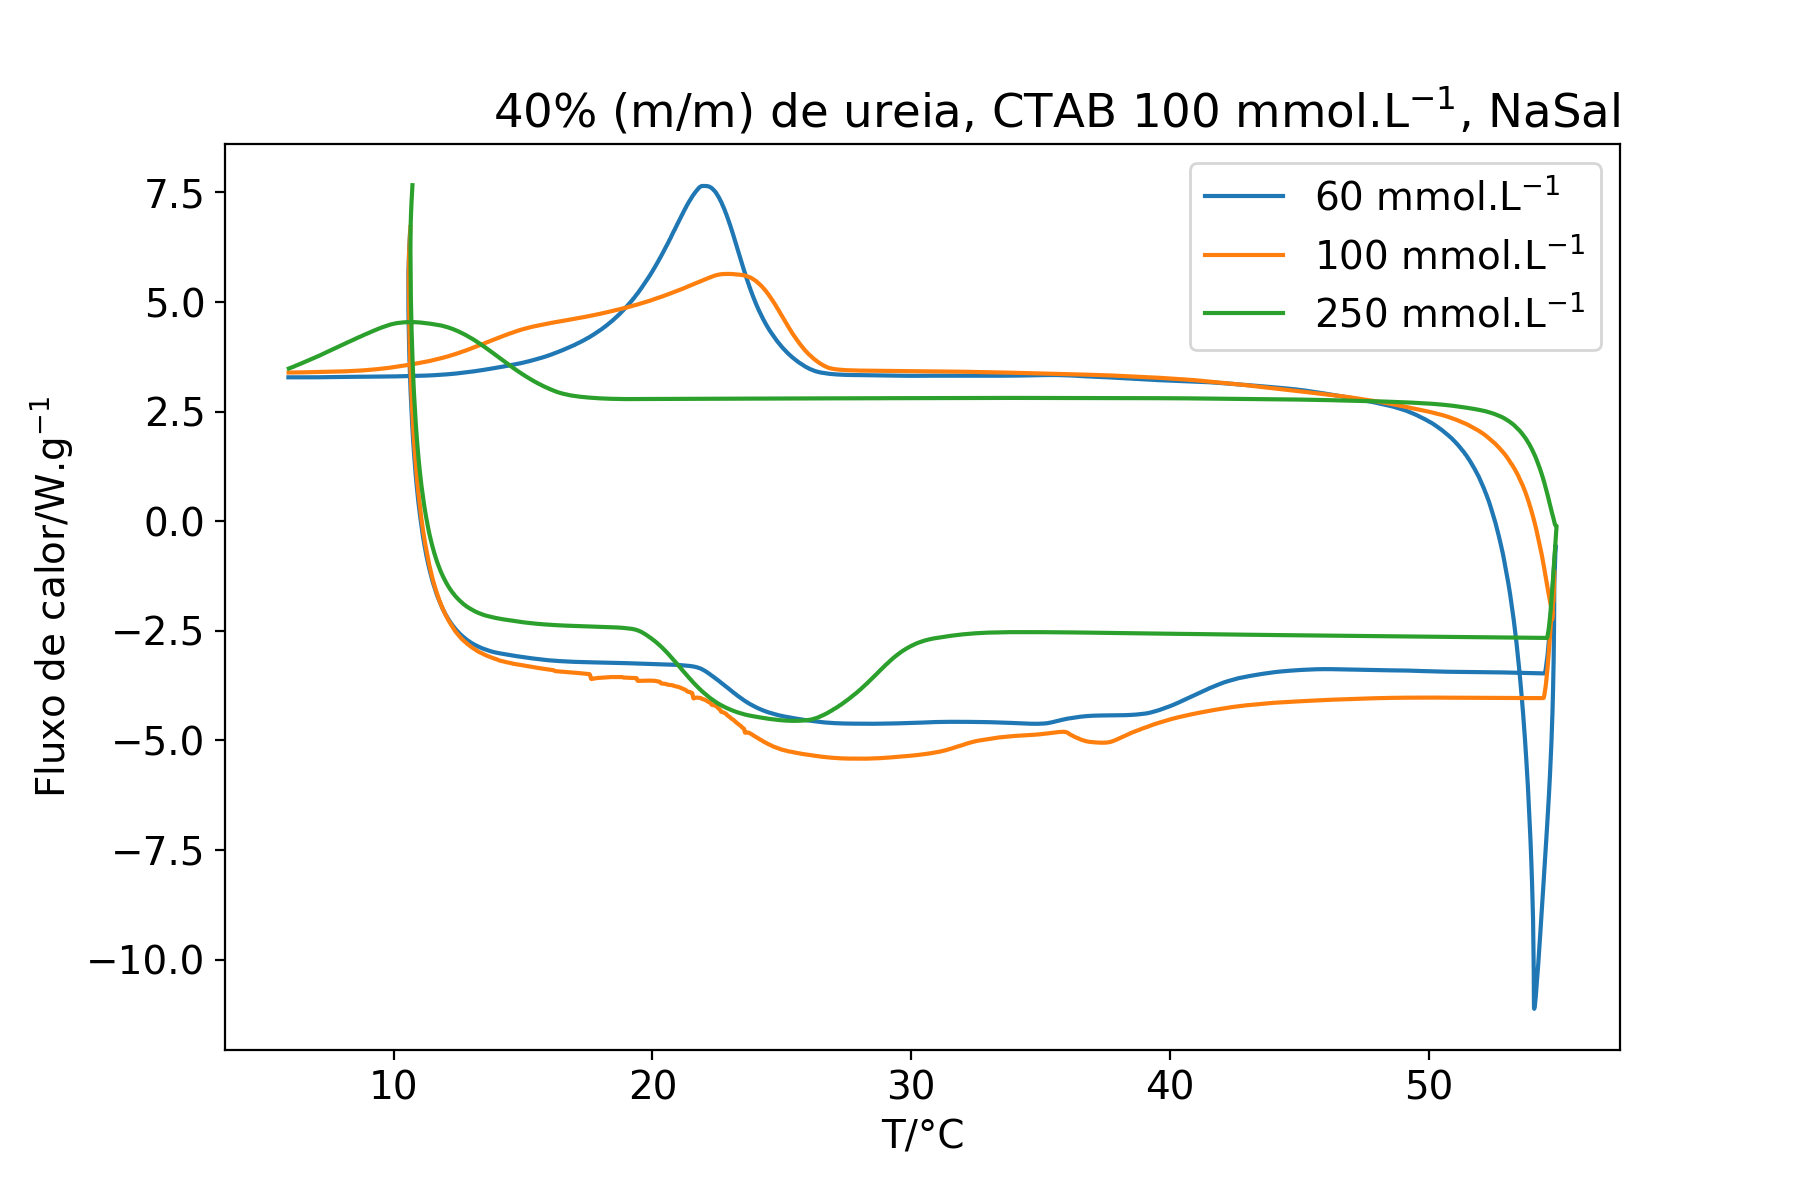
\includegraphics[width=0.60\textwidth]{./imagens/dsc/NaSal40}
%			\caption{Termogramas de soluções de NaSal 60, 100 e 250\mM{} e CTAB 100 \mM{}, em 40\% (m/m) de ureia}
%			\label{fig:DSC_NaSal_Ur40}
%		\end{figure}
%
%		\begin{figure}[H]
%			\centering
%			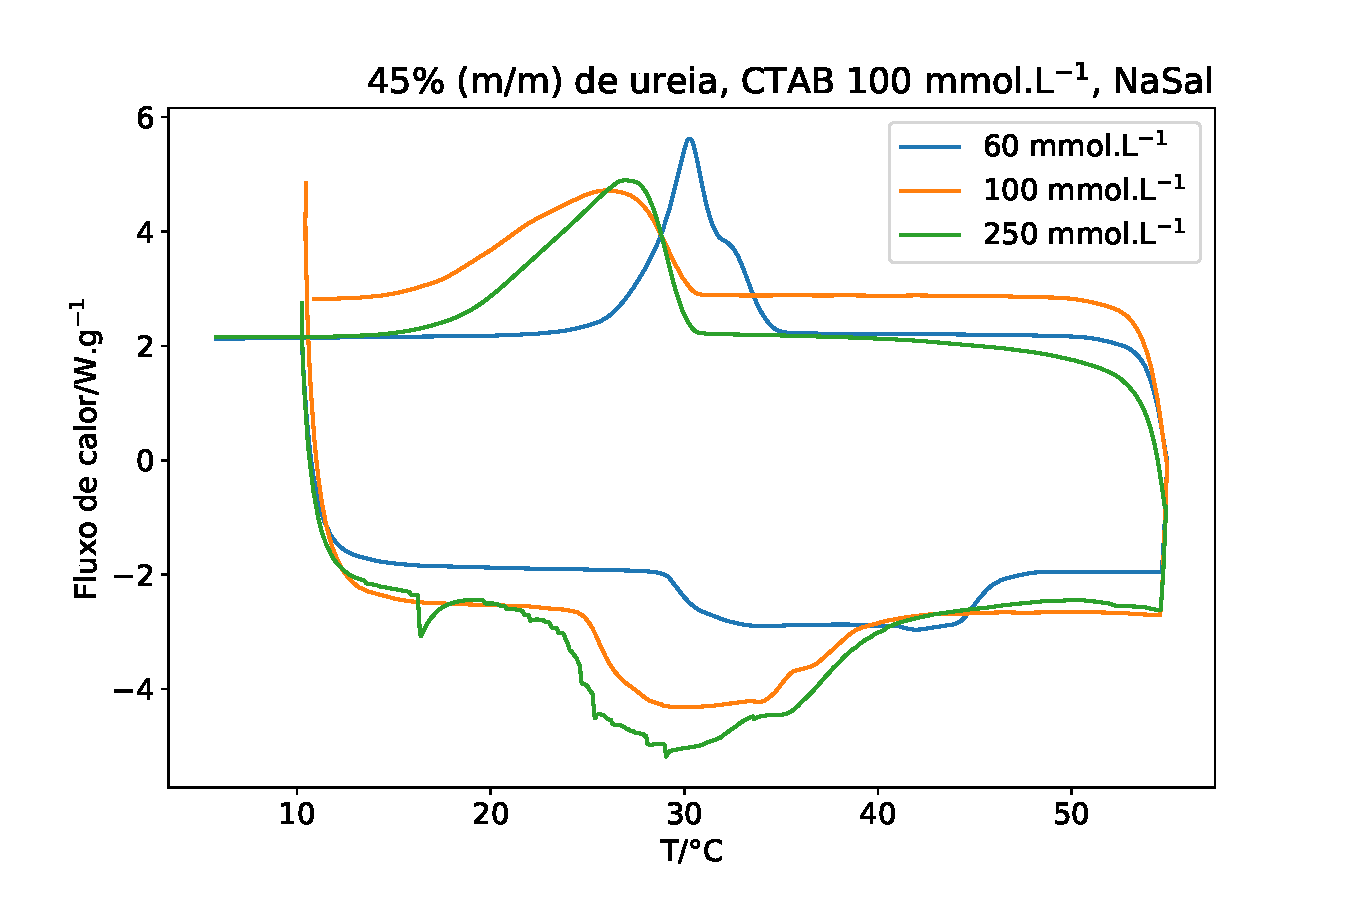
\includegraphics[width=0.60\textwidth]{./imagens/dsc/NaSal45}
%			\caption{Termogramas de soluções de NaSal 60, 100 e 250\mM{} e CTAB 100 \mM{}, em 45\% (m/m) de ureia}
%			\label{fig:DSC_NaSal_Ur45}
%		\end{figure}

		
	% (Figs. \ref{fig:DSC_CTAB_UR38-45}, \ref{fig:DSC_CTAB_UR40-45}, \ref{fig:DSC_TTAB_UR_40-45}, \ref{fig:DSC_DTAB_UR_40-45}, \ref{fig:DSC_NaSal60}, \ref{fig:DSC_NaSal100}, \ref{fig:DSC_NaSal250})
	
	Qualitativamente, pode-se observar que com o aumento de concentração de ureia, a temperatura de transição \(T\) também aumenta. Além disso, com o aumento da concentração de surfactante, a área de transição \(A\) aumenta e fica mais larga. Provavelmente, então, a concentração de ureia se relaciona com a estabilidade dos agregados, mas a concentração de surfactante, na faixa estudada, afeta somente a quantidade de agregados formados. 
	
	A temperatura de transição durante o aquecimento, \(T_{aq}\), é sempre maior que a temperatura de transição no resfriamento, \(T_{res}\). A largura a meia altura, \(L\), segue a mesma tendência. Isso pode estar relacionado com a cinética de desfazer e refazer os agregados. 
	
	Observa-se também que com o aumento na concentração de ureia, \(L\) é pouco afetada, porém \(T\) aumenta gradativamente, já a área \(A\) varia dependendo da natureza do surfactante, com \CTAB{} e \TTAB{} sendo próximos entre si, e diferentes de \DTAB.
	
	A adição de NaSal causa uma diminuição na temperatura de transição, especialmente visível em 250 \mM{} de NaSal. Em vários casos não foi possível medir valores para as áreas de transição de resfriamento.
	
	As Tabelas \ref{tab:DSC_temp_areas} e \ref{tab:DSC_temp_areas_NaSal} mostram as temperaturas de transição no aquecimento e resfriamento, obtidas pelo valor do máximo do pico, as áreas de transição e as larguras a meia altura dos picos de todos os experimentos realizados. A \autoref{fig:DSC_propriedades_Ur_38_45} relaciona as propriedades com a concentração de ureia. % e a figura \ref{fig:DSC_propriedades_NaSal} mostra o efeito de salicilato nas propriedades dos termogramas. % As figuras \ref{fig:DSC_propriedades_surf_40_45} e \ref{fig:DSC_propriedades_surf_40_45_2} relacionam as propriedades dos termogramas em função da concentração de surfactante, a
	
	
    \begin{table}[h]
        \IBGEtab%
        {\caption%
        	[Temperaturas, áreas e larguras a meia altura de \CTAB, \TTAB{} e \DTAB{} em três concentrações de ureia.]%
        	{Temperaturas de transição (\(T\)/°C), áreas de transição por massa de amostra (\(A\)/\(J.g^{-1}\)) e largura a meia altura dos picos de transição (\(L\)/°C) dos ciclos de aquecimento (\emph{aq}) e resfriamento (\emph{res}) para três surfactantes (Surf.), \CTAB, \TTAB, \DTAB, cujas concentrações estão em \mM, em várias concentrações \% (m/m) de ureia}
        \label{tab:DSC_temp_areas}}%
        {\begin{tabular}{ccccccccc}
        	\toprule
        	     Surfactante       &     \(C_{surf}\)     & \% Ureia & \(T_{aq}\) & \(T_{res}\) & \(A_{aq}\) & \(A_{res}\) & \(L_{aq}\) & \(L_{res}\) \\ \midrule
        	\multirow{8}{*}{\CTAB} & \multirow{8}{*}{100} &    38    &    30,5    &    19,3     &    19,4    &    19,5     &    5,6     &     3,0     \\
        	                       &                      &    39    &    32,5    &    25,2     &    22,6    &    22,8     &    6,4     &     2,4     \\
        	                       &                      &    40    &    33,3    &    25,1     &    20,9    &    19,4     &    5,6     &     3,0     \\
        	                       &                      &    41    &    34,1    &    27,2     &    18,1    &    18,4     &    5,3     &     1,6     \\
        	                       &                      &    42    &    37,5    &    29,6     &    19,7    &    20,0     &    6,0     &     1,9     \\
        	                       &                      &    43    &    38,7    &    31,1     &    19,7    &    19,7     &    5,4     &     1,8     \\
        	                       &                      &    44    &    40,2    &    34,6     &    19,7    &    19,7     &    4,9     &     1,6     \\
        	                       &                      &    45    &    41,0    &    34,6     &    20,4    &    20,2     &    4,6     &     1,5     \\ \midrule
        	\multirow{2}{*}{\CTAB} &         200          &    40    &    31,6    &    23,6     &    48,8    &    49,4     &    6,4     &     2,4     \\
        	                       &         200          &    45    &    41,6    &    34,9     &    34,8    &    39,0     &    10,3    &     3,5     \\ \midrule
        	\multirow{8}{*}{\CTAB} & \multirow{8}{*}{300} &    38    &    33,7    &    26,2     &    52,8    &    54,3     &    17,1    &     5,8     \\
        	                       &                      &    39    &    38,2    &    28,3     &    55,8    &    56,6     &    17,2    &     5,1     \\
        	                       &                      &    40    &    40,0    &    29,7     &    52,5    &    54,0     &    15,7    &     5,5     \\
        	                       &                      &    41    &    41,7    &    31,9     &    52,7    &    53,0     &    14,8    &     5,4     \\
        	                       &                      &    42    &    42,9    &    32,8     &    53,7    &    53,2     &    14,1    &     6,3     \\
        	                       &                      &    43    &    44,7    &    35,4     &    53,2    &    52,9     &    13,8    &     6,8     \\
        	                       &                      &    44    &    46,8    &    37,5     &    52,6    &    50,9     &    13,2    &     6,9     \\
        	                       &                      &    45    &    41,4    &    32,8     &    54,4    &    55,2     &    15,4    &     5,8     \\ \midrule
        	\multirow{6}{*}{\TTAB} &         100          &    40    &    31,9    &    26,4     &    11,1    &    10,7     &    4,6     &     1,5     \\
        	                       &         100          &    45    &    37,8    &    34,7     &    11,2    &    11,9     &    4,7     &     1,6     \\
        	                       &         200          &    40    &    31,9    &    25,3     &    23,5    &    22,8     &    10,3    &     3,5     \\
        	                       &         200          &    45    &    37,4    &    33,8     &    25,1    &    25,9     &    8,8     &     2,6     \\
        	                       &         300          &    40    &    29,8    &    26,5     &    34,0    &    35,1     &    15,4    &     5,8     \\
        	                       &         300          &    45    &    37,8    &    33,2     &    38,2    &    39,9     &    14,0    &     4,1     \\ \midrule
        	\multirow{6}{*}{\DTAB} &         100          &    40    &    26,7    &    22,5     &    17,7    &    18,0     &    6,0     &     1,9     \\
        	                       &         100          &    45    &    33,0    &    30,1     &    16,2    &    16,5     &    2,5     &     1,1     \\
        	                       &         200          &    40    &    27,4    &    22,8     &    32,6    &    33,2     &    5,4     &     1,8     \\
        	                       &         200          &    45    &    33,4    &    30,0     &    31,7    &    32,5     &    6,3     &     2,8     \\
        	                       &         300          &    40    &    26,2    &    21,5     &    68,0    &    65,1     &    4,9     &     1,6     \\
        	                       &         300          &    45    &    33,5    &    29,8     &    49,2    &    50,1     &    10,6    &     3,7     \\ \bottomrule
        \end{tabular}}%
        {}
    \end{table}
  % 35  &         CTAB          &    400     &   21,9   &   21,9    &   2,93   &   1,52    &   24,0   &   12,3    \\
  % 40  &         CTAB          &    400     &   36,4   &   26,5    &   2,99   &   1,78    &   23,3   &    7,4    \\
  % 45  &         CTAB          &    400     &   43,4   &   33,6    &   3,79   &   3,74    &   21,7   &    7,4    \\ \midrule 
  
 % \clearpage
  
% todo: verificar a disposição das tabelas aqui, tá meio feio. Será que tem uma maneira de melhorar? Diminuir as figuras ou a legenda da tabela?
  
    \begin{table}[h]
      \IBGEtab%
      {\caption{Temperaturas de transição (\(T\)/°C), áreas de transição por g de amostra (\(A\)/\(J.g^{-1}\)) e largura a meia altura dos picos de transição (\(L\)/°C) dos ciclos de aquecimento (\emph{aq}) e resfriamento (\emph{res}) para \CTAB{} com NaSal, cujas concentrações estão em \mM, em três concentrações \% (m/m) de ureia}
      \label{tab:DSC_temp_areas_NaSal}}%
        {\begin{tabular}{cccccccccc}
        	\toprule
        	\% Ureia &      Surfactante      & \(C_{surf}\) & \(C_{NaSal}\) & \(T_{aq}\) & \(T_{res}\) & \(A_{aq}\) & \(A_{res}\) & \(L_{aq}\) & \(L_{res}\) \\ \midrule
        	   35    & \multirow{9}{*}{\CTAB} &    100     &     60      &   22,0   &   14,6    &   16,5   &   11,33   &    -     &     -     \\
        	   40    &                       &    100     &     60      &   27,6   &   22,0    &   22,2   &   20,56   &    -     &     -     \\
        	   45    &                       &    100     &     60      &   42,0   &   23,5    &   30,3   &   21,69   &   15,0   &    3,0    \\
        	   35    &                       &    100     &     100     &   20,7   &     -     &   19,7   &     -     &   10,9   &     -     \\
        	   40    &                       &    100     &     100     &   27,1   &   22,9    &   22,7   &   18,75   &   15,3   &    9,1    \\
        	   45    &                       &    100     &     100     &   29,9   &   26,0    &   21,6   &   19,08   &   11,0   &    8,5    \\
        	   35    &                       &    100     &     250     &   22,8   &   12,7    &   25,1   &   12,34   &   8,5    &    8,7    \\
        	   40    &                       &    100     &     250     &   23,3   &   11,8    &   18,8   &   10,74   &   7,1    &    7,5    \\
        	   45    &                       &    100     &     250     &   29,1   &   27,0    &   48,6   &   28,85   &   12,3   &    6,9    \\ \bottomrule
        \end{tabular}}%
            {}
    \end{table}

%	\begin{figure}[h]
%	 	\centering
%	 	\begin{subfigure}[t]{0.45\textwidth}
%	 		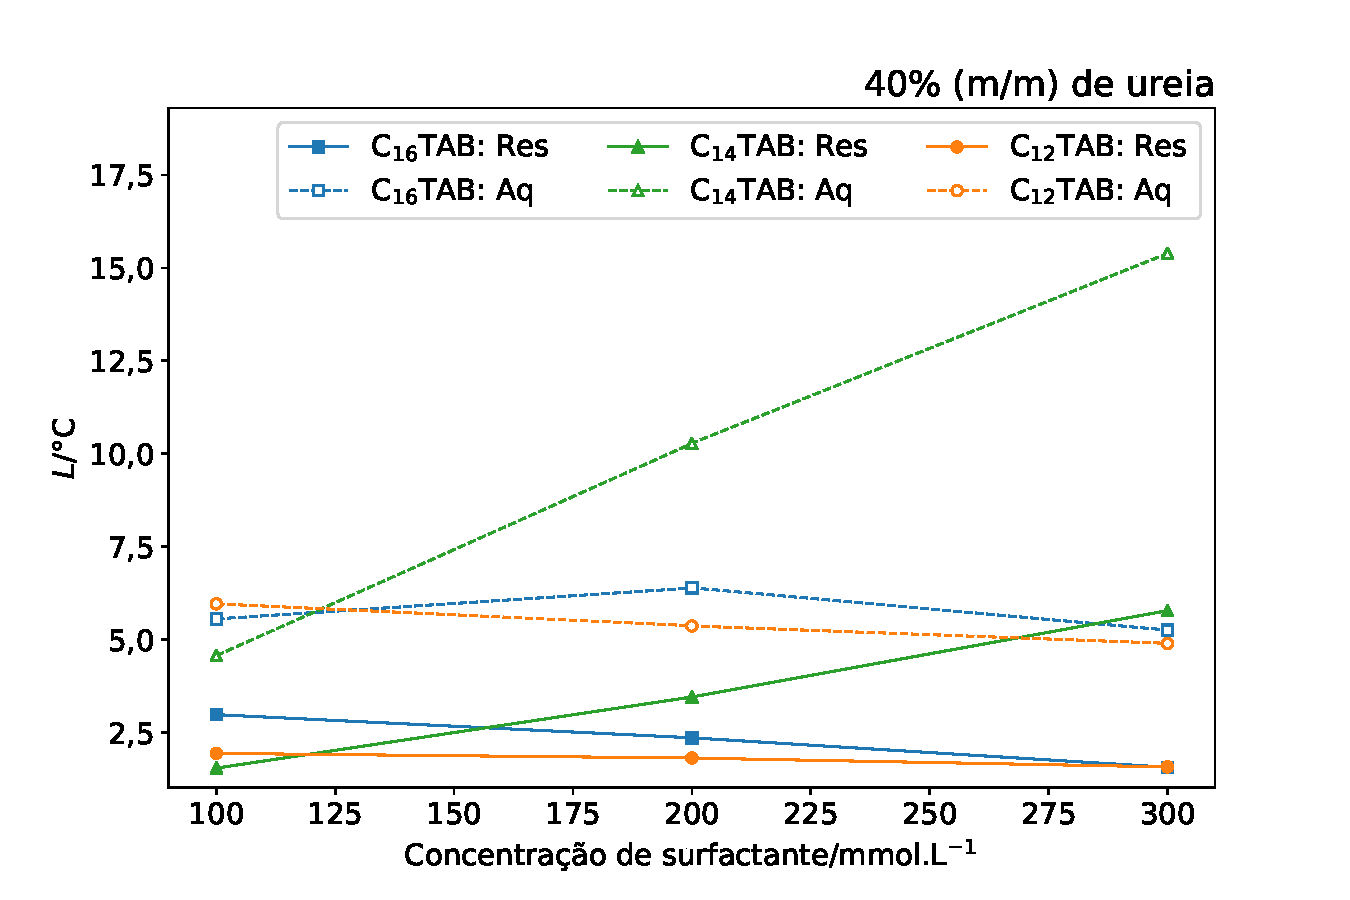
\includegraphics[width=\textwidth]{./imagens/dsc/L_40p_1_300mM_aq_res}
%	 		\caption{\(L\); 40\% de ureia}
%	 		\label{fig:DSC_L_40pUr}
%	 	\end{subfigure} \qquad %
%	 	\begin{subfigure}[t]{0.45\textwidth}
%	 		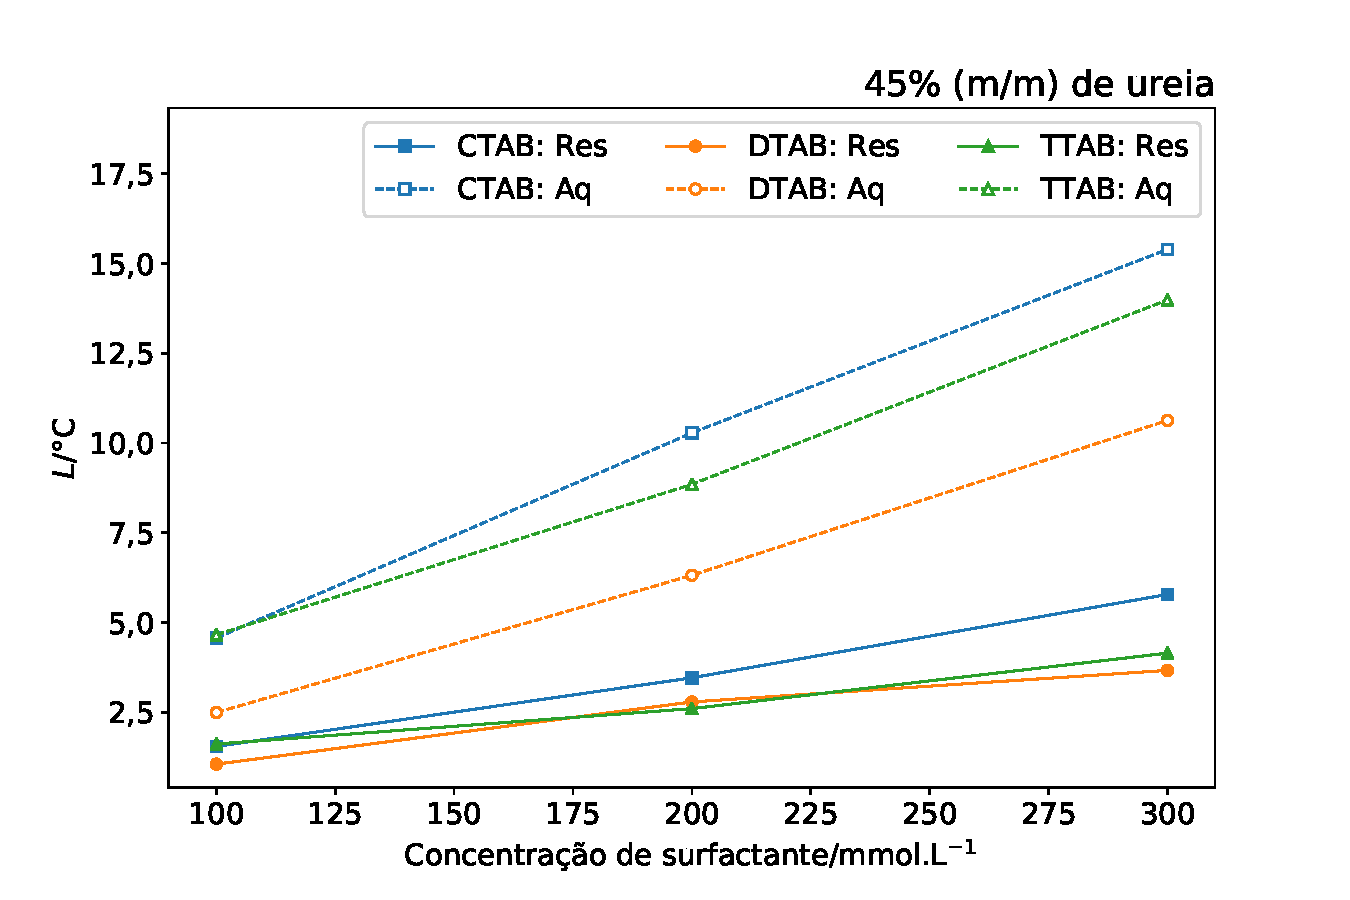
\includegraphics[width=\textwidth]{./imagens/dsc/L_45p_1_300mM_aq_res}
%	 		\caption{\(L\); 45\% de Ureia}
%	 		\label{fig:DSC_L_45pUr}
%	 	\end{subfigure}
% 	
%	 	\begin{subfigure}[t]{0.45\textwidth}
%	 		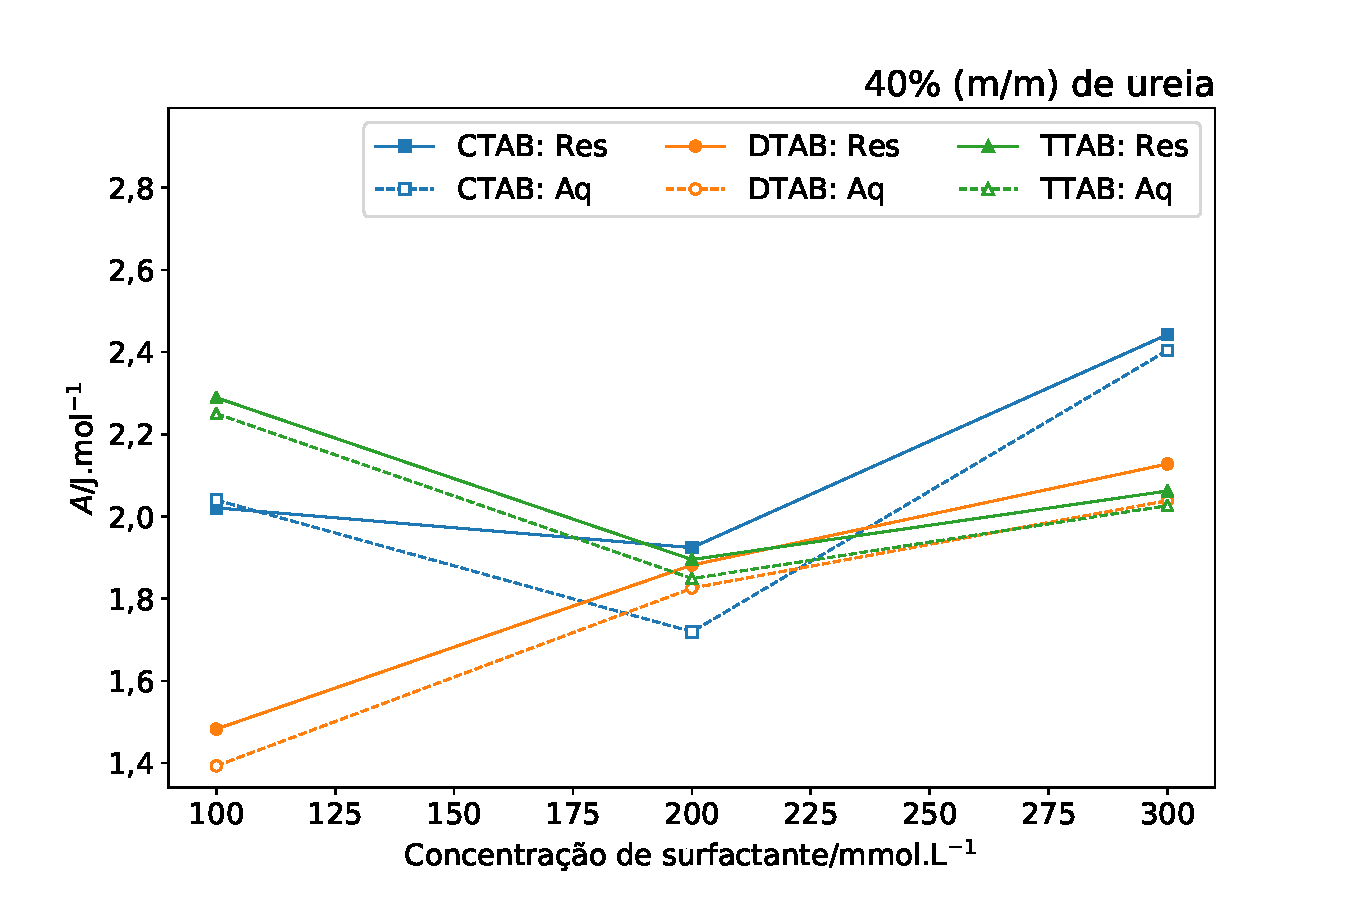
\includegraphics[width=\textwidth]{./imagens/dsc/A_40p_1_300_aq_res}
%	 		\caption{\(A\); 40\% de ureia}
%	 		\label{fig:DSC_A_40pUr}
%	 	\end{subfigure} \qquad %
%	 	\begin{subfigure}[t]{0.45\textwidth}
%	 		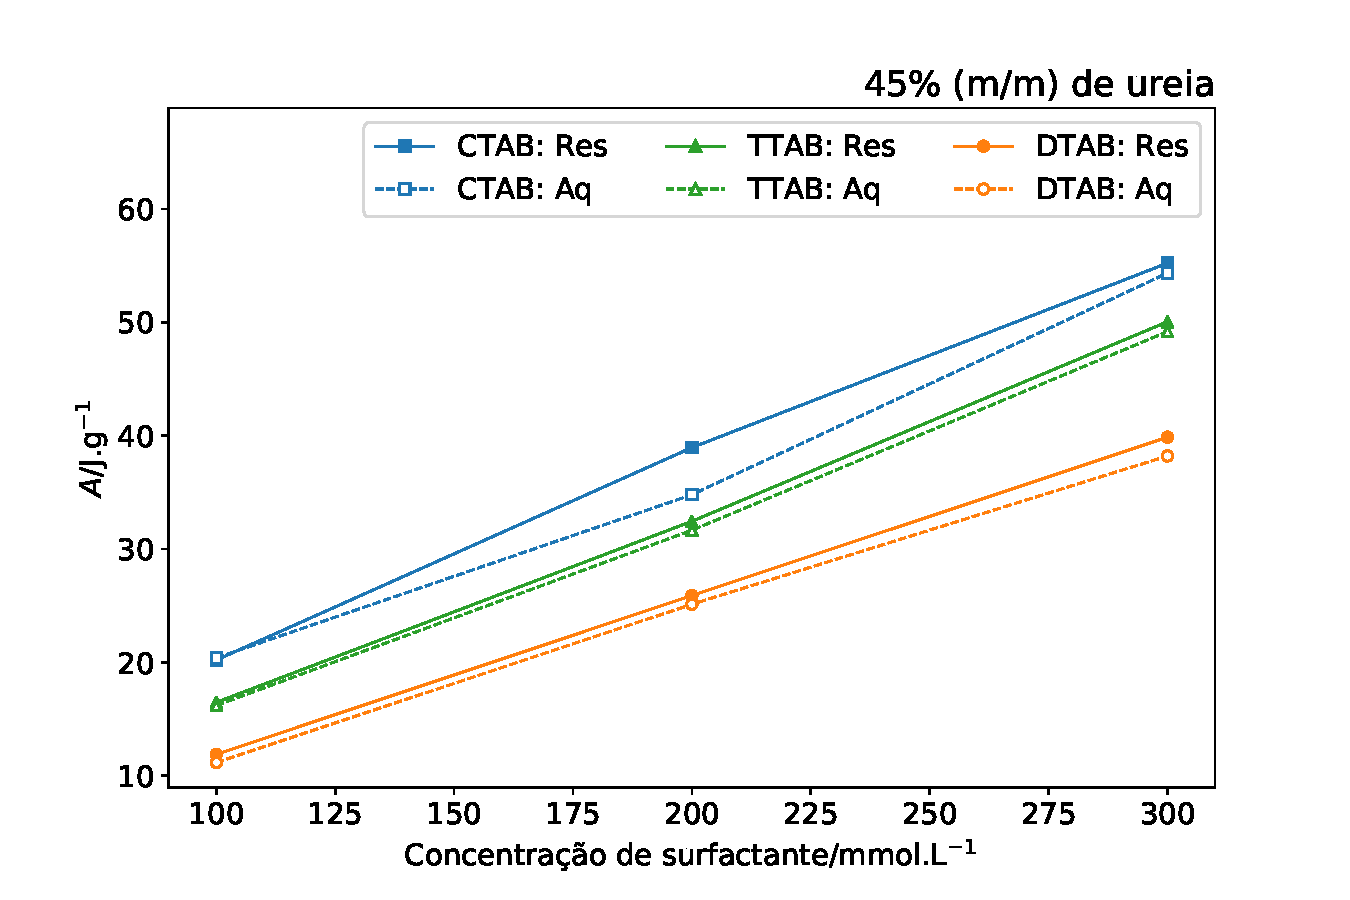
\includegraphics[width=\textwidth]{./imagens/dsc/A_45p_1_300_aq_res}
%	 		\caption{\(A\); 45\% de Ureia}
%	 		\label{fig:DSC_A_45pUr}
%	 	\end{subfigure}
% 	
%	 	\caption{Variação da largura a meia altura \(L\) (\ref{fig:DSC_L_40pUr}, \ref{fig:DSC_L_45pUr}), área do pico \(A\) (\ref{fig:DSC_A_40pUr}, \ref{fig:DSC_A_45pUr}) para os ciclos de aquecimento (\(aq\)) e resfriamento (\(res\)) de amostras de \CTAB, \DTAB{} e \TTAB{} a 35\% e 40\% de ureia, de 100 a 300 \mM{} de surfactante}
%	 	\label{fig:DSC_propriedades_surf_40_45}
%	 \end{figure}
%	
%	\begin{figure}
%	 	\begin{subfigure}[t]{0.45\textwidth}
%			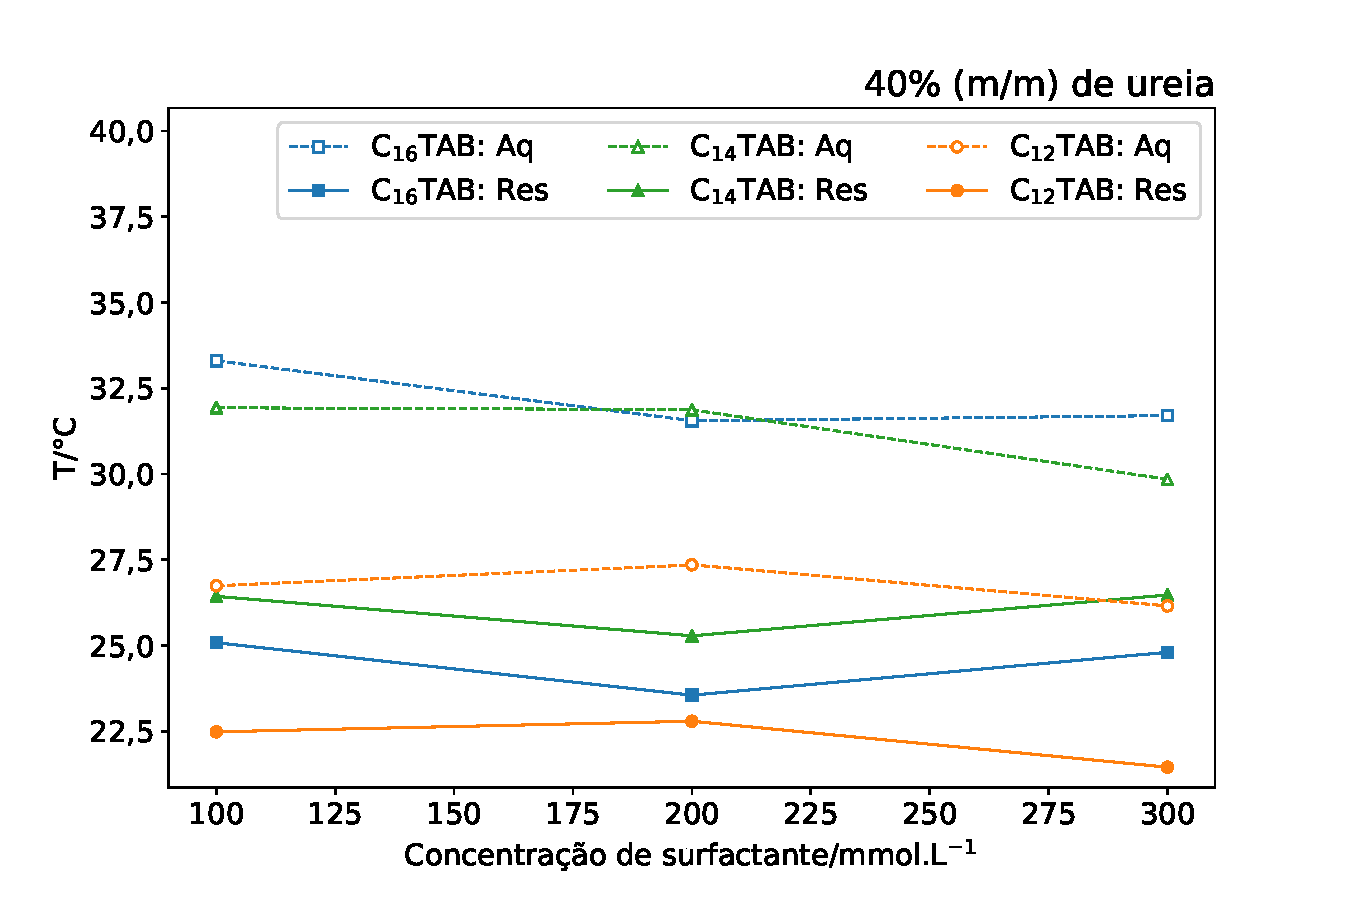
\includegraphics[width=\textwidth]{./imagens/dsc/T_40p_1_300_aq_res}
%			\caption{\(T\); 40\% de ureia}
%			\label{fig:DSC_T_40pUr}
%		\end{subfigure}  %
%		\begin{subfigure}[t]{0.45\textwidth}
%			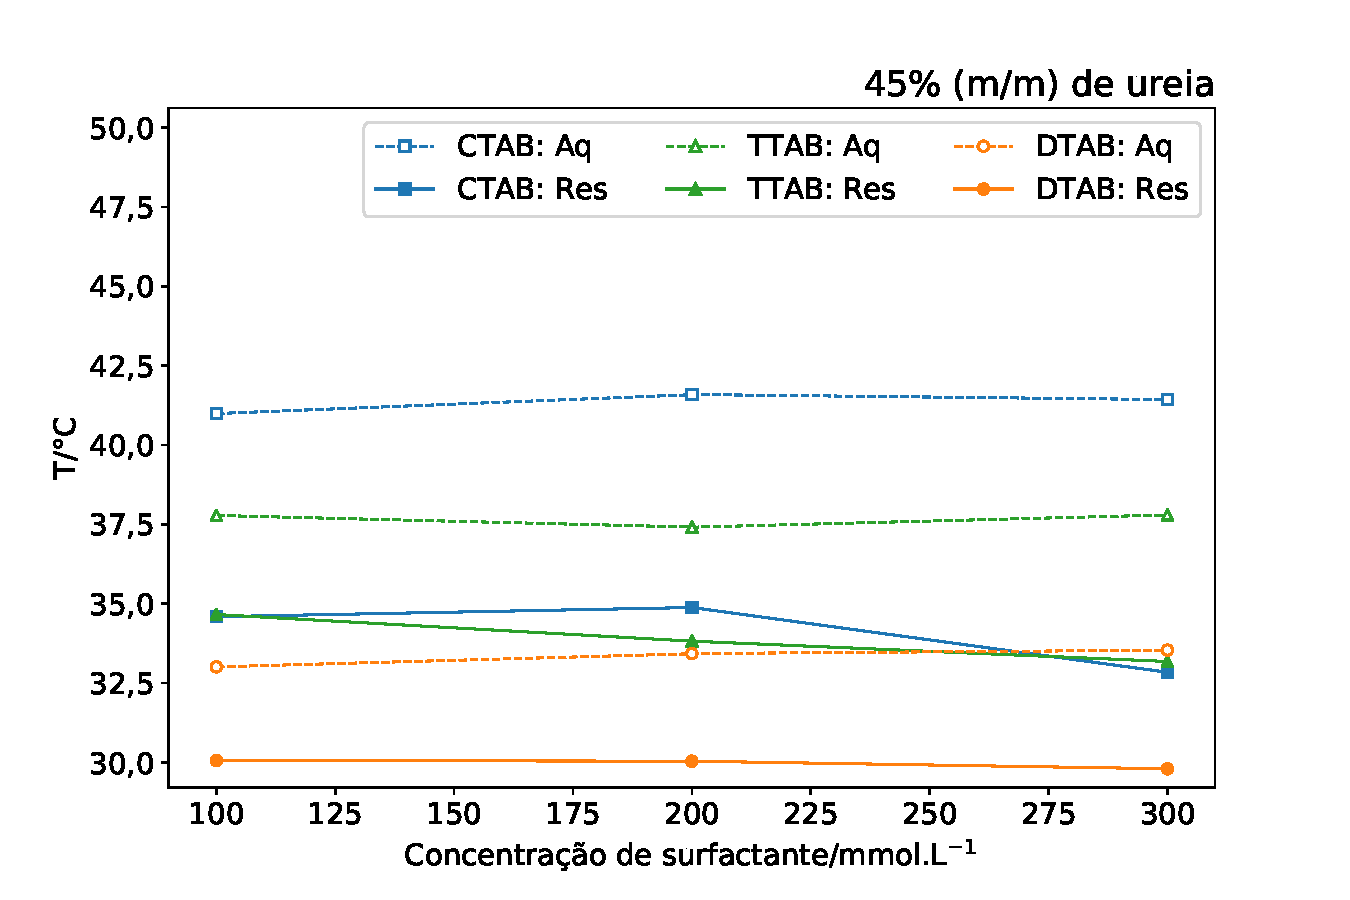
\includegraphics[width=\textwidth]{./imagens/dsc/T_45p_1_300_aq_res}
%			\caption{\(T\); 45\% de Ureia}
%			\label{fig:DSC_T_45pUr}
%		\end{subfigure}
%	 
%	 	\caption{Variação da temperatura de transição \(T\) (\ref{fig:DSC_T_40pUr}, \ref{fig:DSC_T_45pUr}) para os ciclos de aquecimento (\(aq\)) e resfriamento (\(res\)) de amostras de \CTAB, \DTAB{} e \TTAB{} a 35\% e 40\% de ureia, de 100 a 300 \mM{} de surfactante}
%		\label{fig:DSC_propriedades_surf_40_45_2}
%	\end{figure}
	
	
	\begin{figure}[h]	
		\begin{subfigure}[t]{0.5\textwidth}
			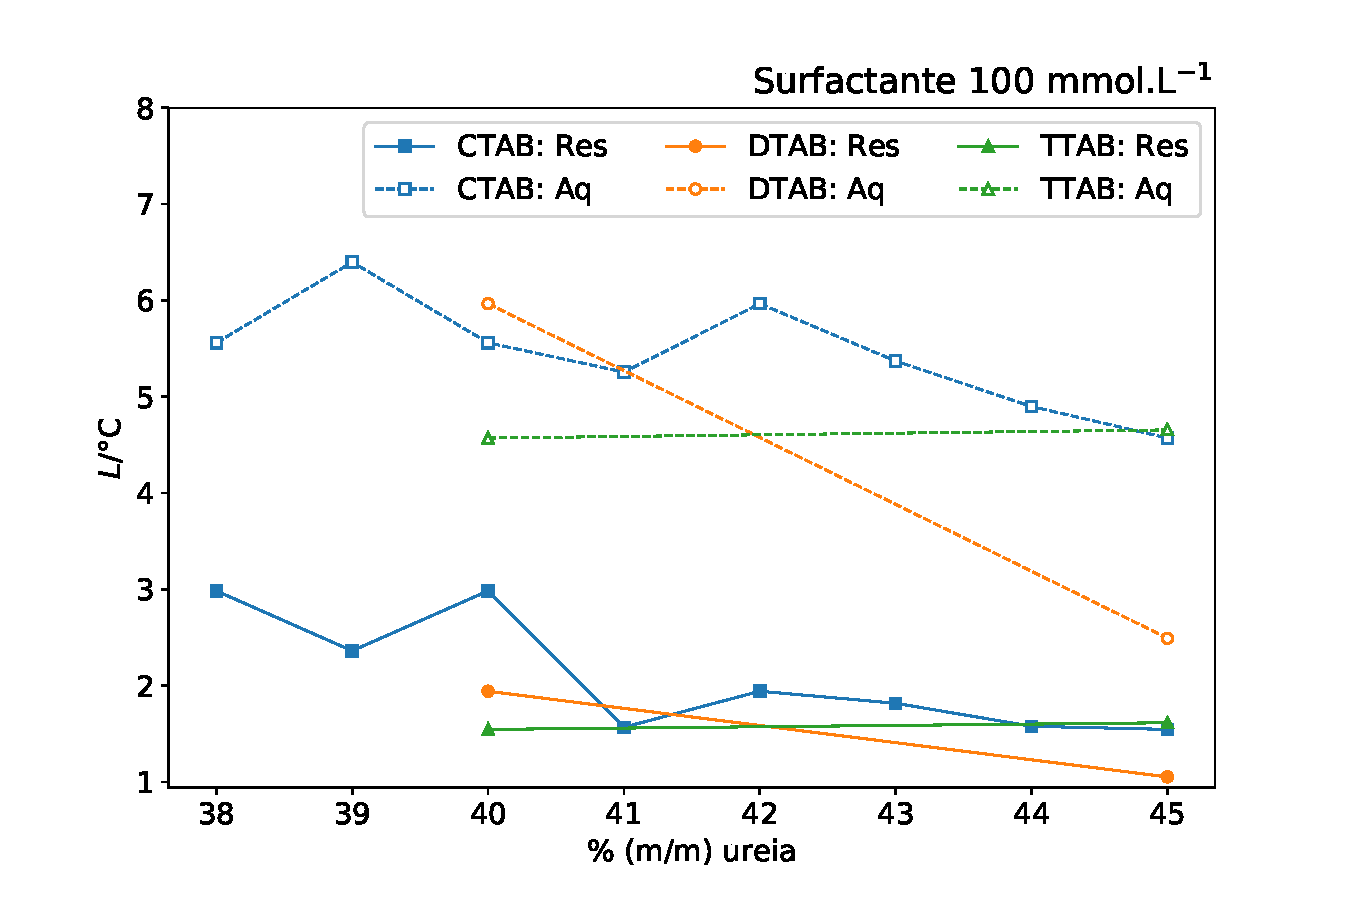
\includegraphics[width=\textwidth]{./imagens/dsc/L_100mM_aq_res}
			\caption{\(L\) a 38\%---45\% de ureia}
			\label{fig:DSC_L_38_45pUr}
		\end{subfigure} %
		%
		\begin{subfigure}[t]{0.5\textwidth}
			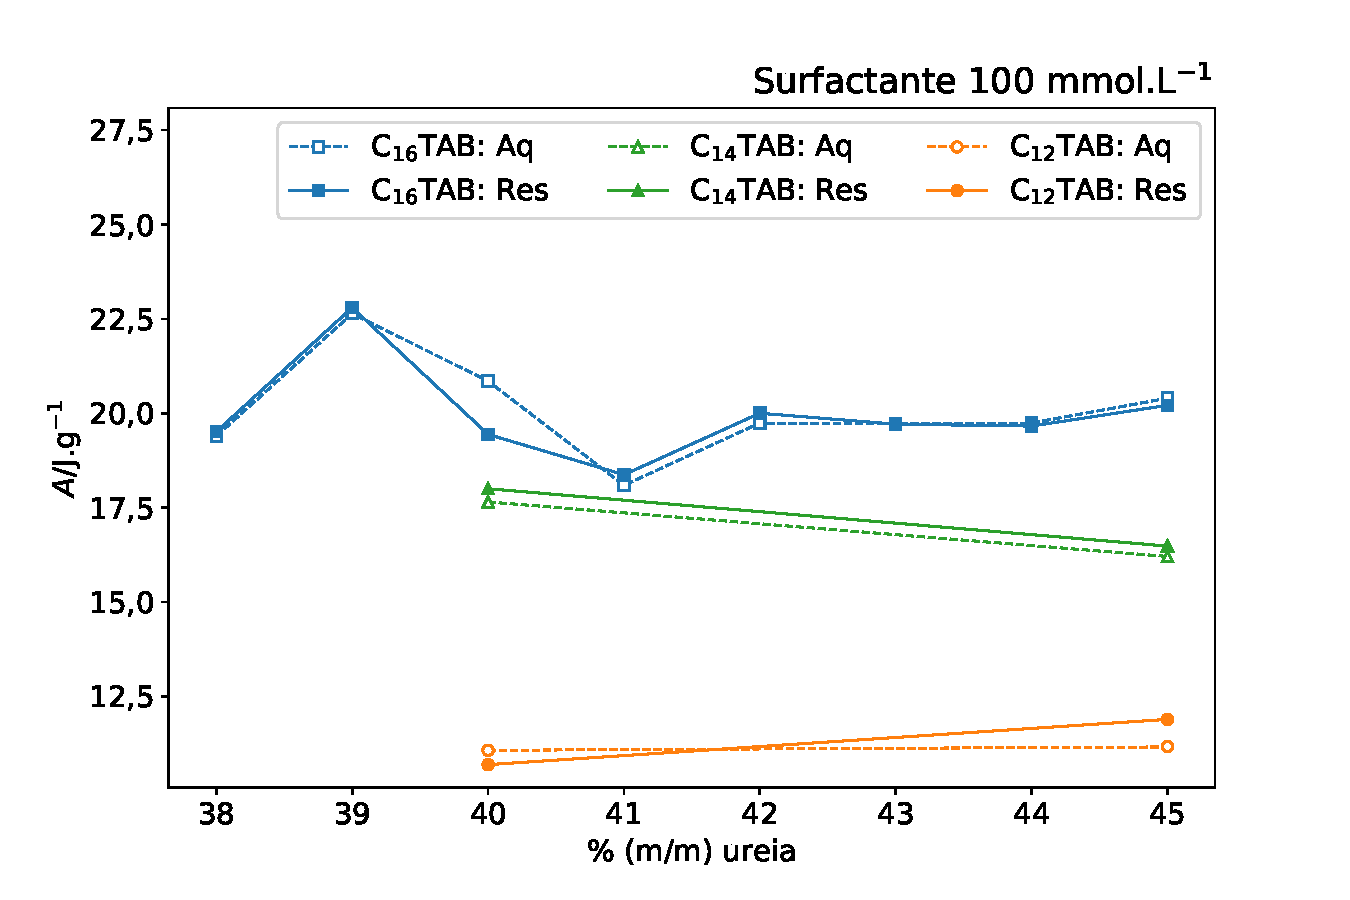
\includegraphics[width=\textwidth]{./imagens/dsc/A_100mM_aq_res}
			\caption{\(A\) a 38\%---45\% de ureia}
			\label{fig:DSC_A_38_45pUr}
		\end{subfigure} 
		
		\hspace{4cm} \begin{subfigure}[t]{0.5\textwidth}
			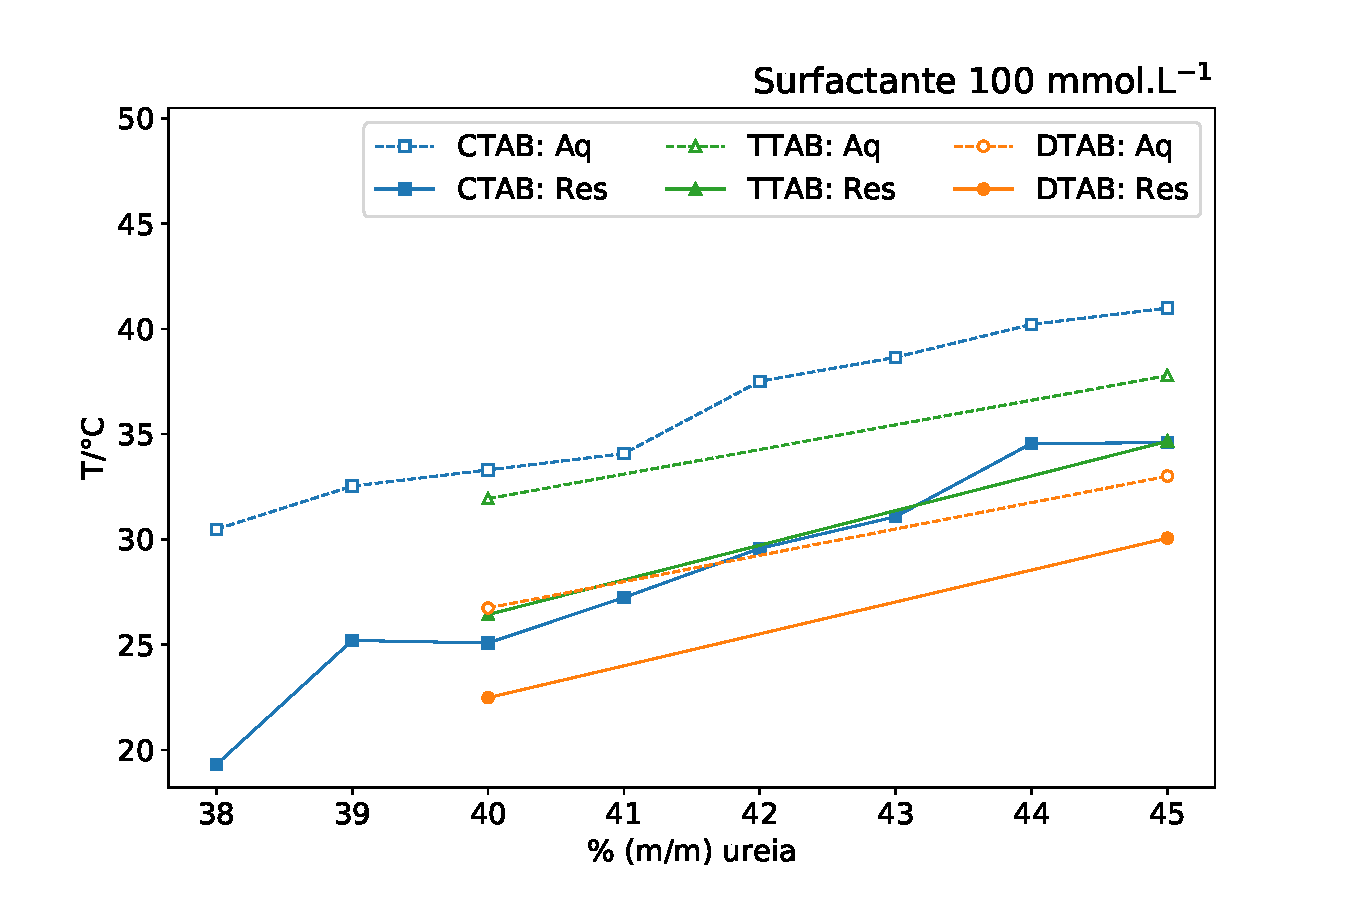
\includegraphics[width=\textwidth]{./imagens/dsc/T_100mM_aq_res}
			\caption{\(T\) a 38\%---45\% de ureia}
			\label{fig:DSC_T_38_45pUr}
		\end{subfigure}
		
		\caption{Variação da largura a meia altura \(L\) (\ref{fig:DSC_L_38_45pUr}), área do pico \(A\) (\ref{fig:DSC_A_38_45pUr}), temperatura de transição \(T\) (\ref{fig:DSC_T_38_45pUr}) para os ciclos de aquecimento \(aq\) e resfriamento \(res\) de amostras de \CTAB, \DTAB{} e \TTAB{} de 38\% a 45\% de ureia e 100 \mM{} de surfactante.}
		\label{fig:DSC_propriedades_Ur_38_45}
	\end{figure}
		
%	\begin{figure}[h]
%		\centering
%		\begin{subfigure}[t]{0.45\textwidth}
%			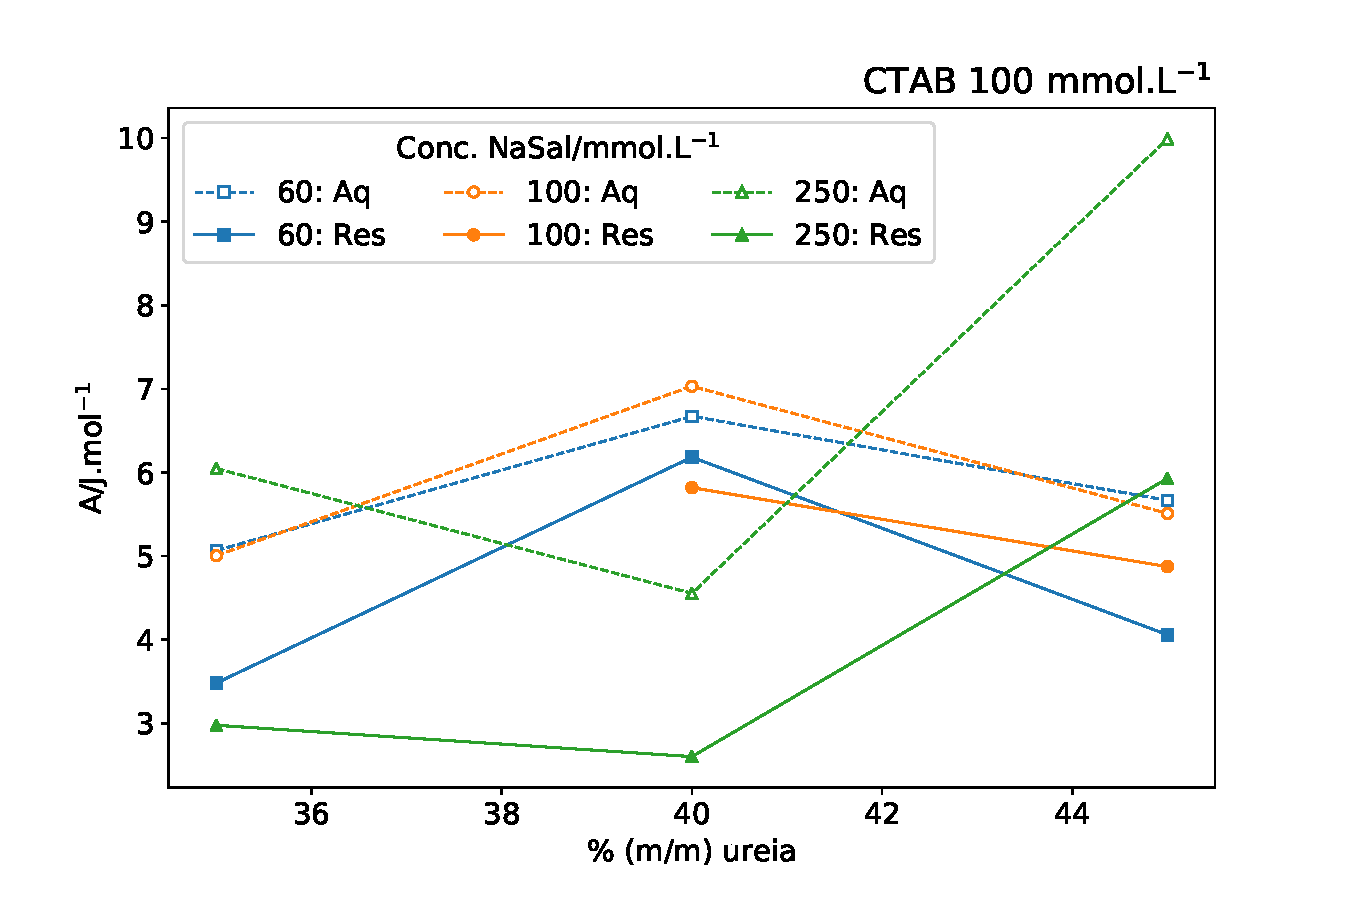
\includegraphics[width=\textwidth]{./imagens/dsc/A_NaSal_c_UR_aq_res}
%			\caption{\(A\) a 35\% de ureia}
%			\label{fig:DSC_A_NaSal}
%		\end{subfigure} \qquad %
%		\begin{subfigure}[t]{0.45\textwidth}
%			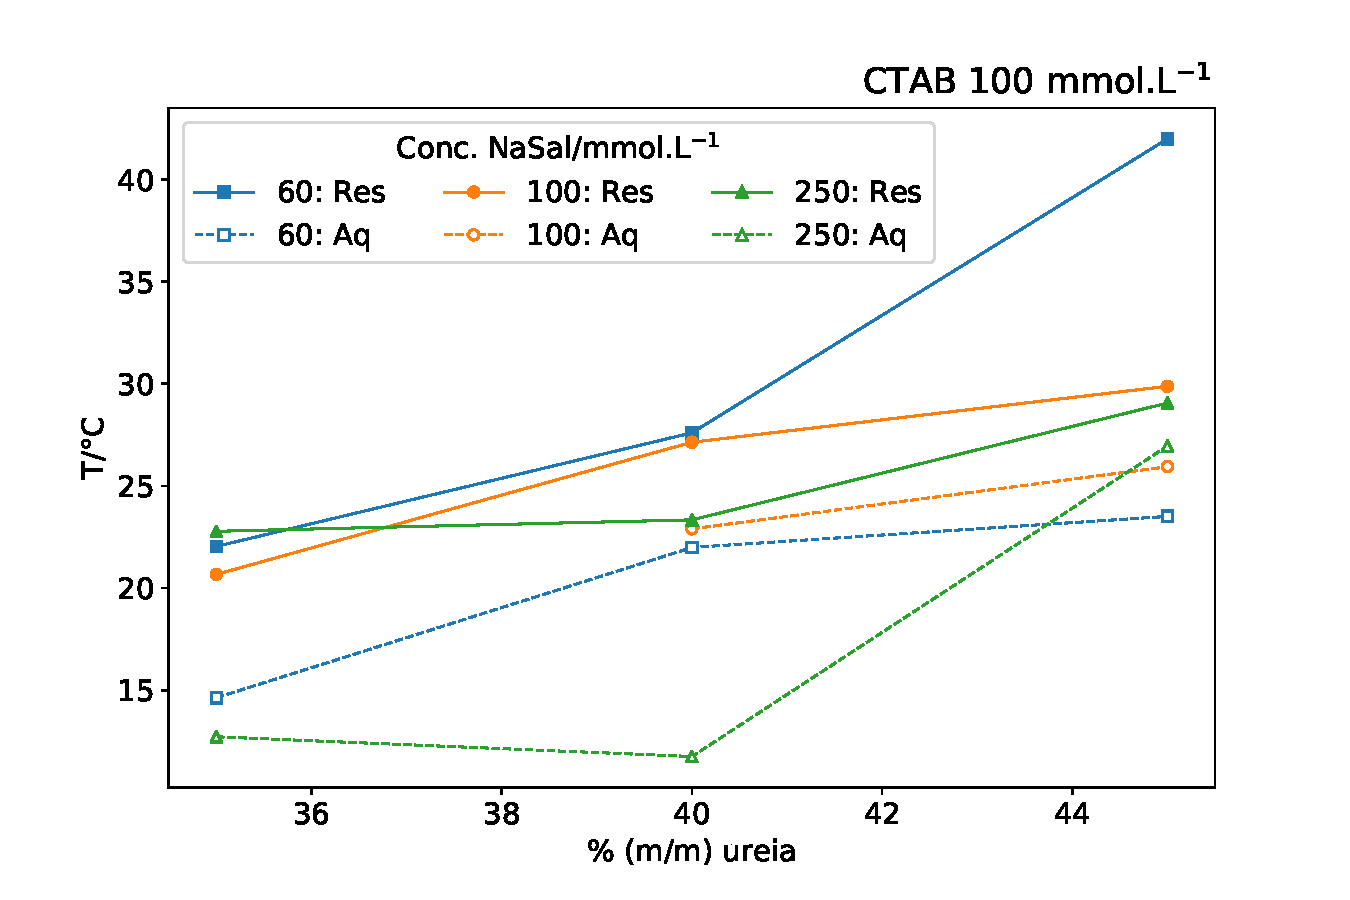
\includegraphics[width=\textwidth]{./imagens/dsc/T_NaSal_c_UR_aq_res}
%			\caption{\(T\) a 40\% de Ureia}
%			\label{fig:DSC_T_NaSal}
%		\end{subfigure}
%		
%		\caption{Variações da área do pico \(A\) (\ref{fig:DSC_A_NaSal}), temperatura de transição \(T\) (\ref{fig:DSC_T_NaSal}) para os ciclos de aquecimento (\(aq\)) e resfriamento (\(res\)) de amostras de \CTAB{} e NaSal a 35\% a 40\% de ureia, de 60 a 250 \mM{} de NaSal}
%		\label{fig:DSC_propriedades_NaSal}
%	\end{figure}
	
	\FloatBarrier
\section{SAXS} \index{resultados!SAXS}

	Foram realizadas análises de SAXS para determinar a estrutura da fase branca. O papel do comprimento da cadeia e da concentração de surfactante foram avaliados (Figuras \ref{fig:SAXS_ctabconc}, \ref{fig:SAXS_ttabconc}, \ref{fig:SAXS_dtabconc}).
	
	\begin{figure}[h]
		\centering
		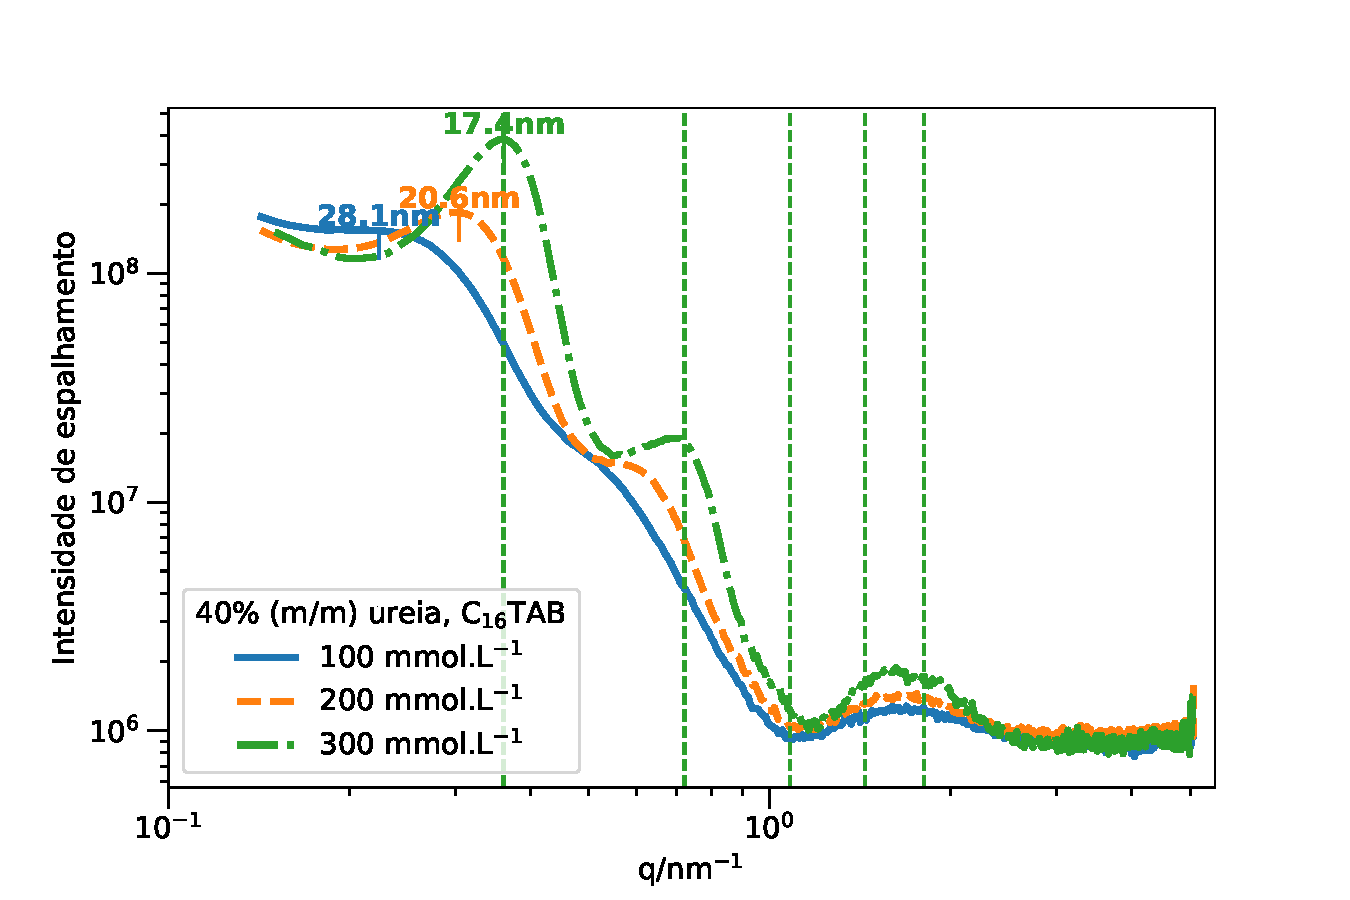
\includegraphics[width=0.7\textwidth]{imagens/saxs/CTAB_conc}
		\caption{Curvas de SAXS de \CTAB{} 100, 200 e 300 \mM{} e 40\% (m/m) de ureia. Os parâmetros de rede foram calculados com o primeiro pico. As retas verticais indicam as posições \(1:2:3\dots\) em relação ao primeiro pico.}
		\label{fig:SAXS_ctabconc}
	\end{figure}
	
	\begin{figure}[h]
		\centering
		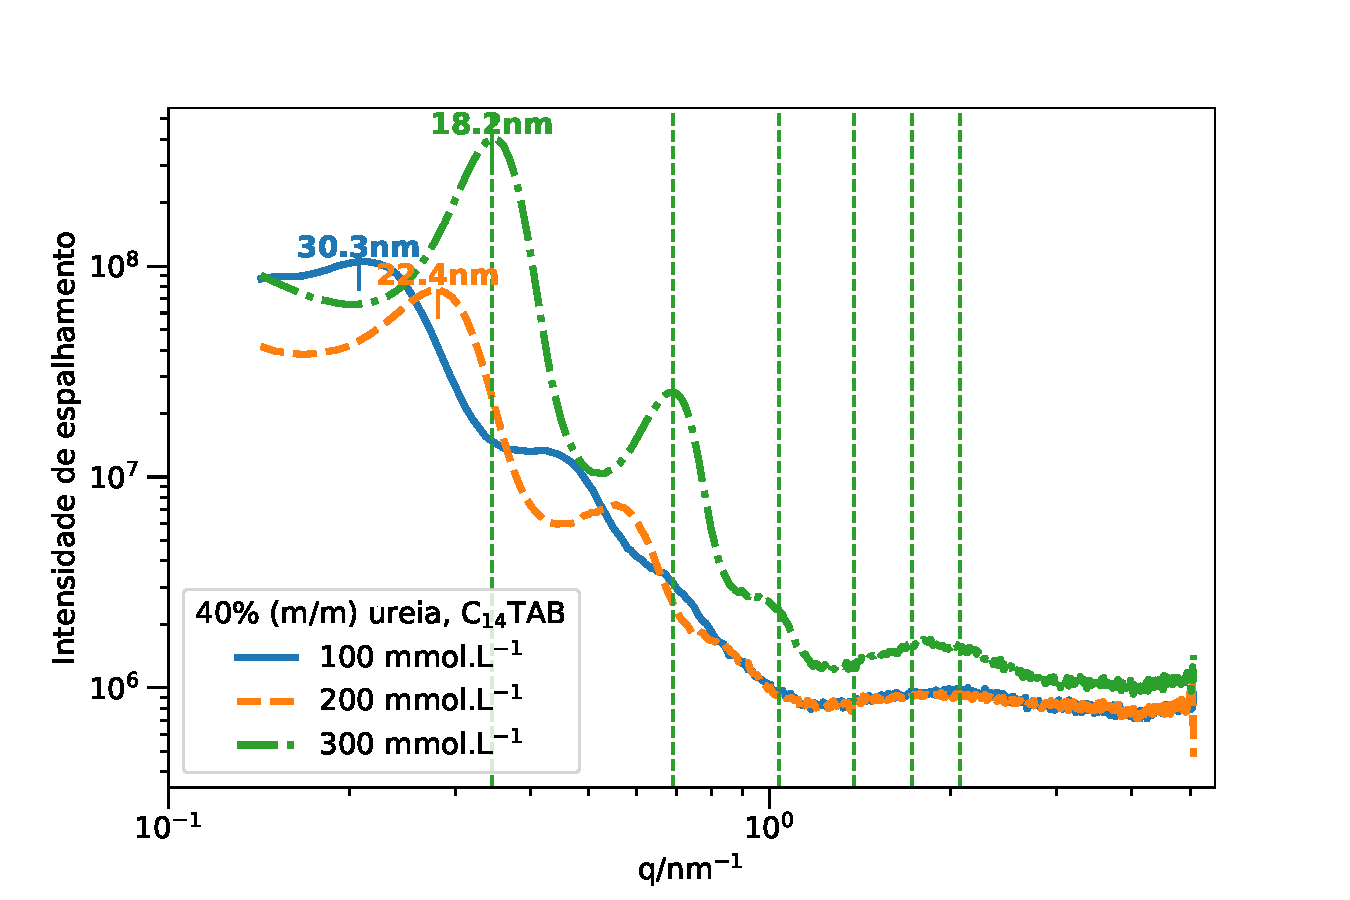
\includegraphics[width=0.7\textwidth]{imagens/saxs/TTAB_conc}
		\caption{Curvas de SAXS de \TTAB{} 100, 200 e 300 \mM{} e 40\% (m/m) de ureia. Os parâmetros de rede foram calculados com o primeiro pico. As retas verticais indicam as posições \(1:2:3\dots\) em relação ao primeiro pico.}
		\label{fig:SAXS_ttabconc}
	\end{figure}
	
	\begin{figure}[h]
		\centering
		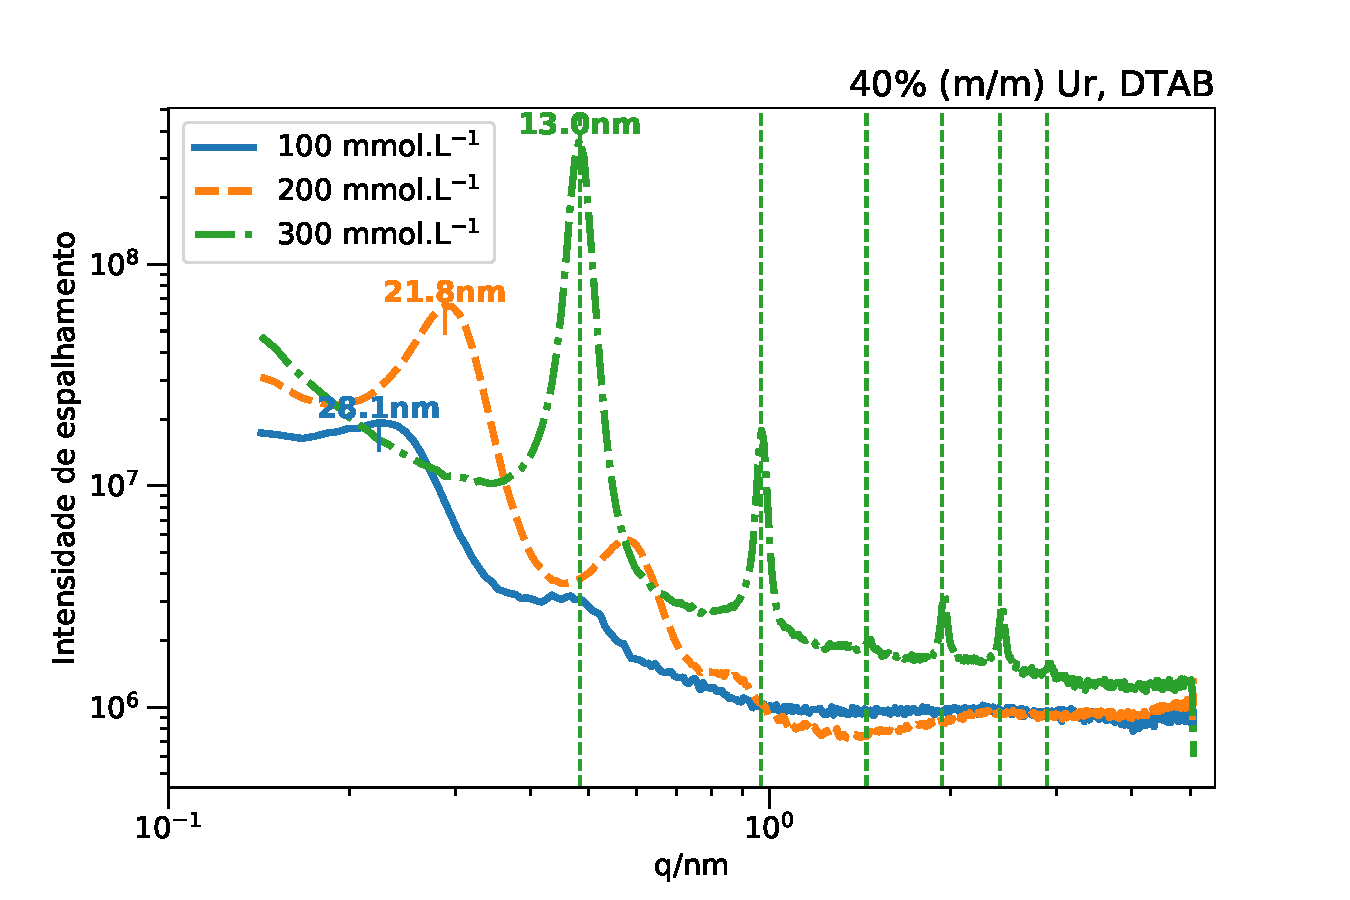
\includegraphics[width=0.7\textwidth]{imagens/saxs/DTAB_conc}
		\caption{Curvas de SAXS de \DTAB{} 100, 200 e 300 \mM{} e 40\% (m/m) de ureia. Os parâmetros de rede foram calculados com o primeiro pico. As retas verticais indicam as posições \(1:2:3\dots\) em relação ao primeiro pico.}
		\label{fig:SAXS_dtabconc}
	\end{figure}
	
	Para analisar a fase presente, é necessário indexar os picos, como informado na \autoref{sec:teoria_SAXS}. Isto é, determinar os valores de \q{} de seus máximos e observar a relação entre eles. Lamelas possuem espaçamento \(1:2:3\), e como em todas as curvas mostradas aqui seguem esse espaçamento, podemos concluir que todas as amostras formam lamelas. Com a \autoref{eqn:SAXS_param_rede_lamela} é possível determinar a distância de rede das lamelas, que é a distância entre o início de uma lamela, passando pela parte hidrofóbica e pelo solvente até atingir a superfície de outra lamela.

	As distâncias de repetição estão ilustradas junto com os valores dos picos nas figuras. É possível observar que as distâncias se tornam menores a medida que a concentração de surfactante aumenta, possivelmente porque mais surfactante resulta também em menos solvente. Além disso, é possível que a carga das micelas se torne menor devido à presença de mais contraíons em solução. Observa-se também que os picos se tornam melhor definidos e aparentemente menos largos com mais surfactante. É interessante notar que \DTAB{} possui picos muito bem definidos em 300 \mM, e que sua distância de repetição é muito menor que os outros casos. A espessura dos picos está inversamente relacionada com o tamanho dos ``cristalitos'', de acordo com a equação de Scherrer.\cite{Kockrick2008} Logo, o aumento de concentração de surfactante também aumenta o tamanho dos cristalitos.
	
	Também foi analisado o efeito da concentração de ureia em amostras de 300 \mM{} de \CTAB{} (\autoref{fig:SAXS_ctab300ur37-45}). Interessantemente, a adição de ureia aparenta diminuir o tamanho dos cristalitos, tanto que o trio de picos na faixa de \q{} acima de 1 nm\textsuperscript{-1} se junta, formando uma banda só em concentrações de ureia acima de 39\%. Observamos também que a distância de repetição é um pouco afetada pela adição de ureia, aumentando de 14,5 para 18,3 nm.
	
	Além disso, foram analisadas amostras a 50°C para obter informações sobre a fase transparente (\autoref{fig:SAXS_surf50c}). Observa-se que os padrões de espalhamento se alteraram drasticamente, e que o padrão para \CTAB{} e \TTAB{} são bastante diferentes. Não foi possível medir \DTAB{} pois havia muito pouco contraste.
	
	\begin{figure}[h]
		\centering
		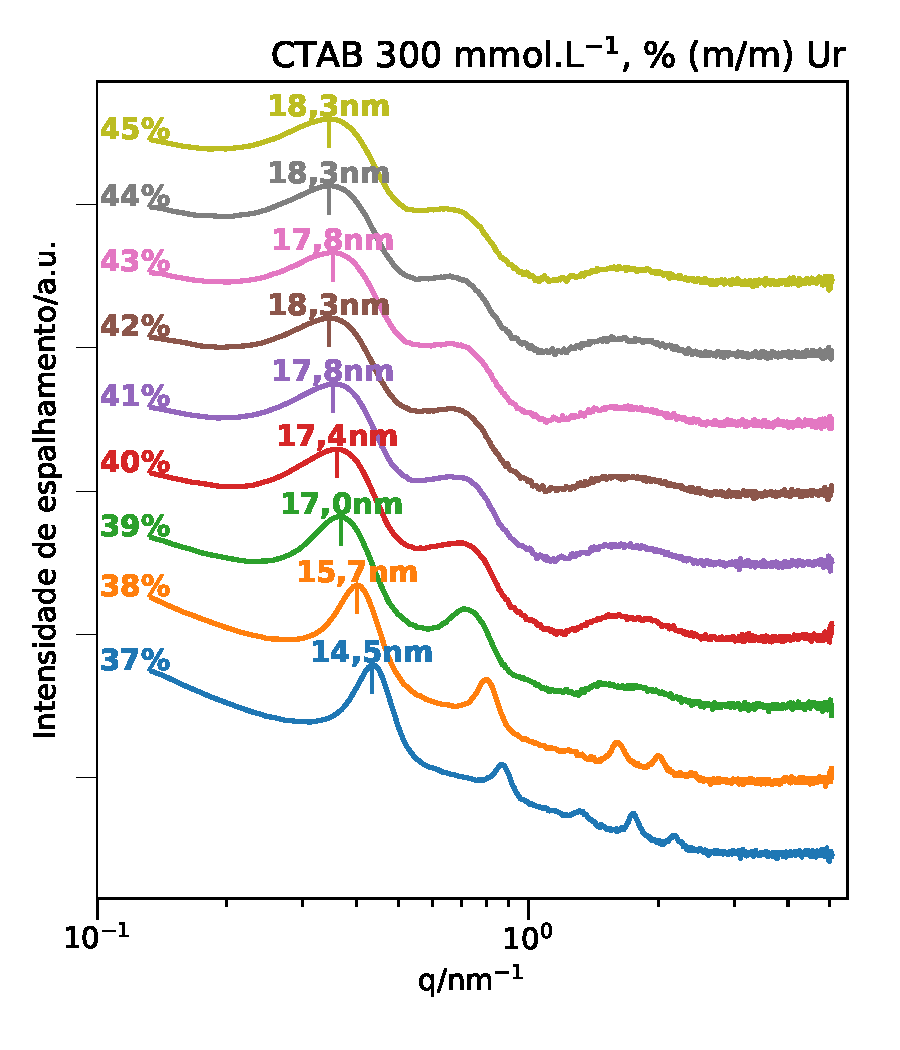
\includegraphics[width=0.5\textwidth]{imagens/saxs/CTAB300Ur37-45}
		\caption{Curvas de SAXS de \CTAB{} 300 \mM{} em concentrações crescentes de ureia, com os parâmetros de rede calculados com o primeiro pico.}
		\label{fig:SAXS_ctab300ur37-45}
	\end{figure}
	
	\begin{figure}[h]
		\centering
		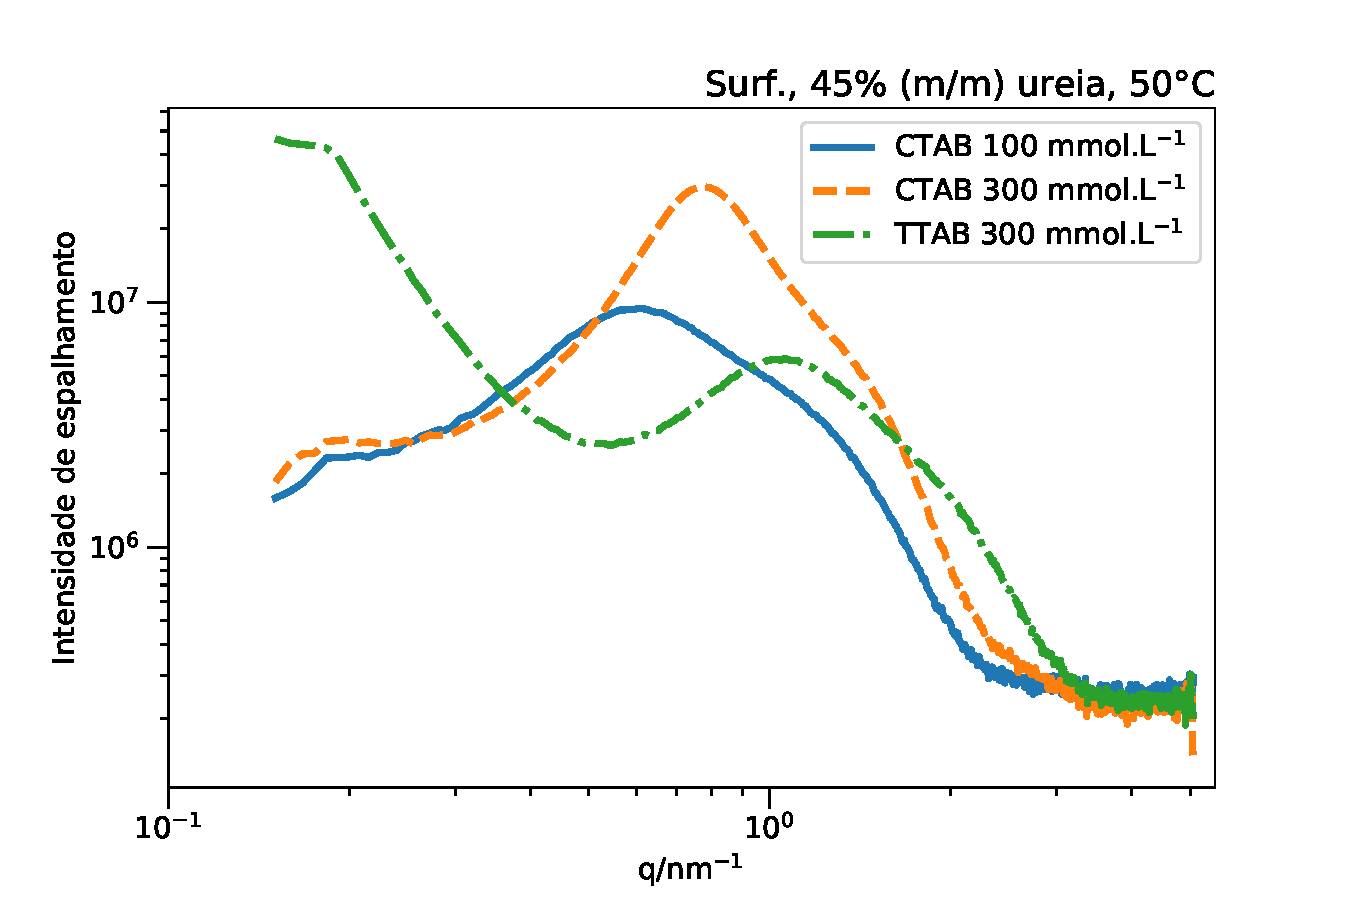
\includegraphics[width=0.7\textwidth]{imagens/saxs/Surf_50C}
		\caption{Curvas de SAXS de \CTAB{} 100 e 300 \mM{} e \TTAB{} 300 \mM{} com 45\% de ureia, a 50°C. As distâncias de correlação no pico foram calculadas.}
		\label{fig:SAXS_surf50c}
	\end{figure}

	Em temperaturas elevadas, as soluções são pouco viscosas, transparentes e isotrópicas. Essas características sugerem que há alguma estrutura como micelas esféricas, micelas cilíndricas curtas ou vesículas nessas soluções. Seria interessante comparar os perfis de espalhamento da estruturas similares, e a maneira mais fácil de realizar isso é medir soluções com a mesma concentração de surfactante, mas sem ureia. A \autoref{fig:SAXS_micelas_esfericas} mostra os padrões de espalhamento de micelas em água para os três surfactantes, a 100, 200 e 300 \mM.
	
	\begin{figure}[h]
		\centering
		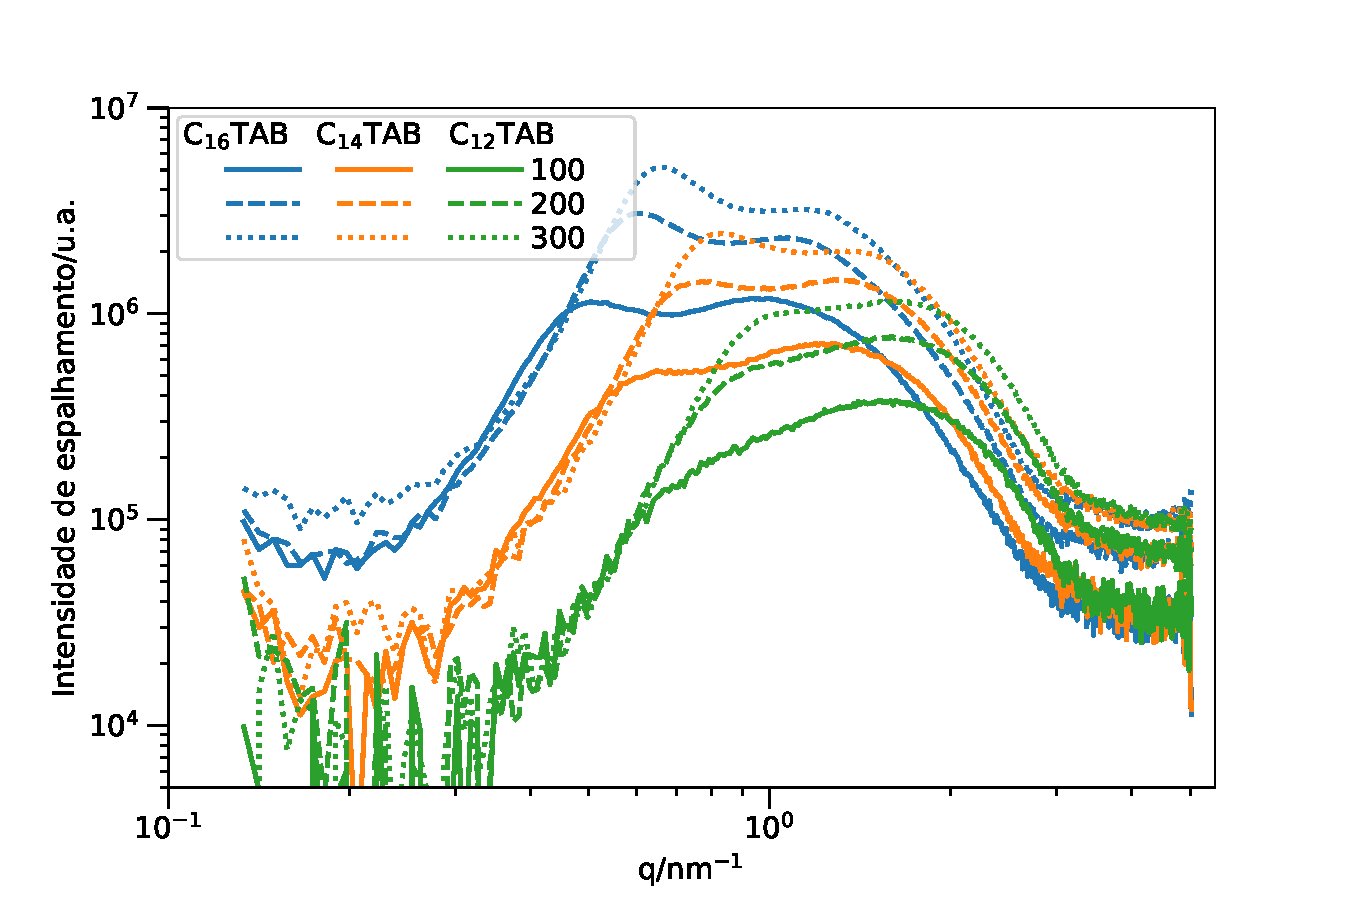
\includegraphics[width=0.7\textwidth]{imagens/saxs/micelas_esfericas}
		\caption{Curvas de SAXS de \CTAB, \TTAB{} e \DTAB{} 100, 200 e 300 \mM{} em água, mostrando o perfil característico de micelas globulares carregadas.}
		\label{fig:SAXS_micelas_esfericas}
	\end{figure}
	
	Observa-se o perfil característico de micelas carregadas, com um pico do correlação \(q_\mathrm{corr}\) em valores de \q{} menores e outro pico estrutural \(q_\mathrm{estr}\).\cite{Lutz-Bueno2017} Quanto mais carregadas forem as micelas, menor será a distância de correlação  A \autoref{fig:SAXS_ctab_q_corrs} evidencia os picos de correlação. 
	
	\begin{figure}[h]
		\centering
		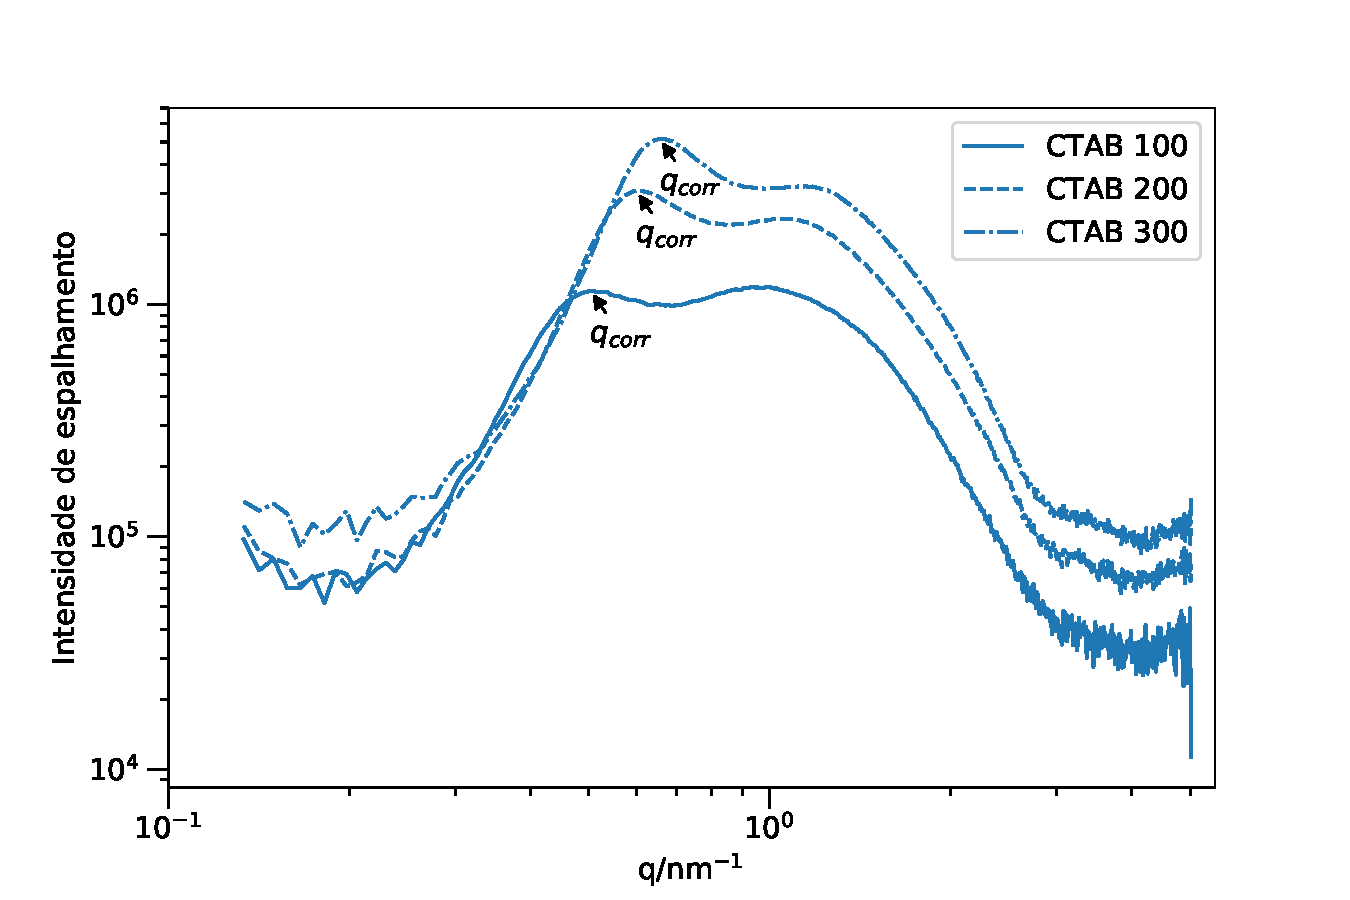
\includegraphics[width=0.7\textwidth]{imagens/saxs/CTAB_q_corrs}
		\caption{Curvas de SAXS de \CTAB{} 100, 200 e 300 \mM{} em água, evidenciando os picos de correlação.}
		\label{fig:SAXS_ctab_q_corrs}
	\end{figure}

	Utilizando a \autoref{eqn:SAXS_param_rede_lamela}, é possível encontrar a distância intermicelar média. A \autoref{tab:SAXS_dim} mostra as distâncias intermicelares calculadas por esse método.
	
%	\begin{table}
%		\IBGEtab%
%		{\caption{Distâncias intermicelares \(d_{im}\) de soluções de micelas esféricas de (C|T|D)TAB 100, 200, 300 \mM{} calculadas a partir da eq. \ref{eqn:SAXS_param_rede}}
%		\label{tab:SAXS_dim}}%
%		{\begin{tabular}{p{3cm} p{3cm} p{0.1cm}}
%			\toprule
%			\centering Solução  & \centering \(d_{im}\)/nm & \\ 
%			\midrule
%			\centering CTAB 100  & \centering  12,5    & \\
%			\centering CTAB 200  & \centering  10,4    & \\
%			\centering CTAB 300  & \centering  9,57    & \\ 
%			\midrule
%			\centering TTAB 100  & \centering 9,71    & \\
%			\centering TTAB 200  & \centering 8,26    & \\
%			\centering TTAB 300  & \centering 7,55    & \\ 
%			\midrule
%			\centering DTAB 100  & \centering 9,44    & \\
%			\centering DTAB 200  & \centering 7,14    & \\
%			\centering DTAB 300  & \centering 6,31    & \\ 
%			\bottomrule
%		\end{tabular}}%
%		{}
%	\end{table} % todo: pensar se é possível estruturar essa tabela com Surf nas linhas e conc nas colunas, ou o contrário.
%	% por algum motivo esta coluna extra na tabela é necessária.
	
		\begin{table}[h]
		\IBGEtab%
		{\caption{Distâncias intermicelares \(d_{im}\)/nm de soluções de micelas esféricas de \CTDTAB{} 100, 200, 300 \mM{} calculadas a partir da \autoref{eqn:SAXS_param_rede_lamela}}
			\label{tab:SAXS_dim}}%
		{\begin{tabular}{c | c c c}
			\toprule
			Concentração/\mM & \CTAB  & \TTAB & \DTAB  \\ \midrule
			    100      & 12,5 & 9,7 & 9,5 \\
			    200      & 10,5 & 8,3 & 7,1 \\
			    300      & 9,5 & 7,6 & 6,3 \\ \bottomrule
		\end{tabular}}%
		{}
	\end{table}
	
	Observamos então que a distância intermicelar diminui com o aumento da concentração de surfactante. Isso é esperado, uma vez que mais micelas estão presentes e, possivelmente, a presença de uma maior quantidade de contraíons diminui a carga superficial micelar, logo a repulsão intermicelar diminui. Considerando esse fato, há uma semelhança entre as curvas das soluções de surfactante com ureia a 50°C (\autoref{fig:SAXS_surf50c}) e as soluções de surfactante em água a 25°C (\autoref{fig:SAXS_micelas_esfericas}). Se as micelas estiverem com menos íons adsorvidos, o pico de correlação \(q_{corr}\) se tornará mais intenso, sendo possível até encobrir o pico estrutural. As curvas estão comparadas na \autoref{fig:SAXS_com_sem_ureia}.

	
	\begin{figure}[h]
		\begin{subfigure}[t]{0.5\textwidth}
			\centering
			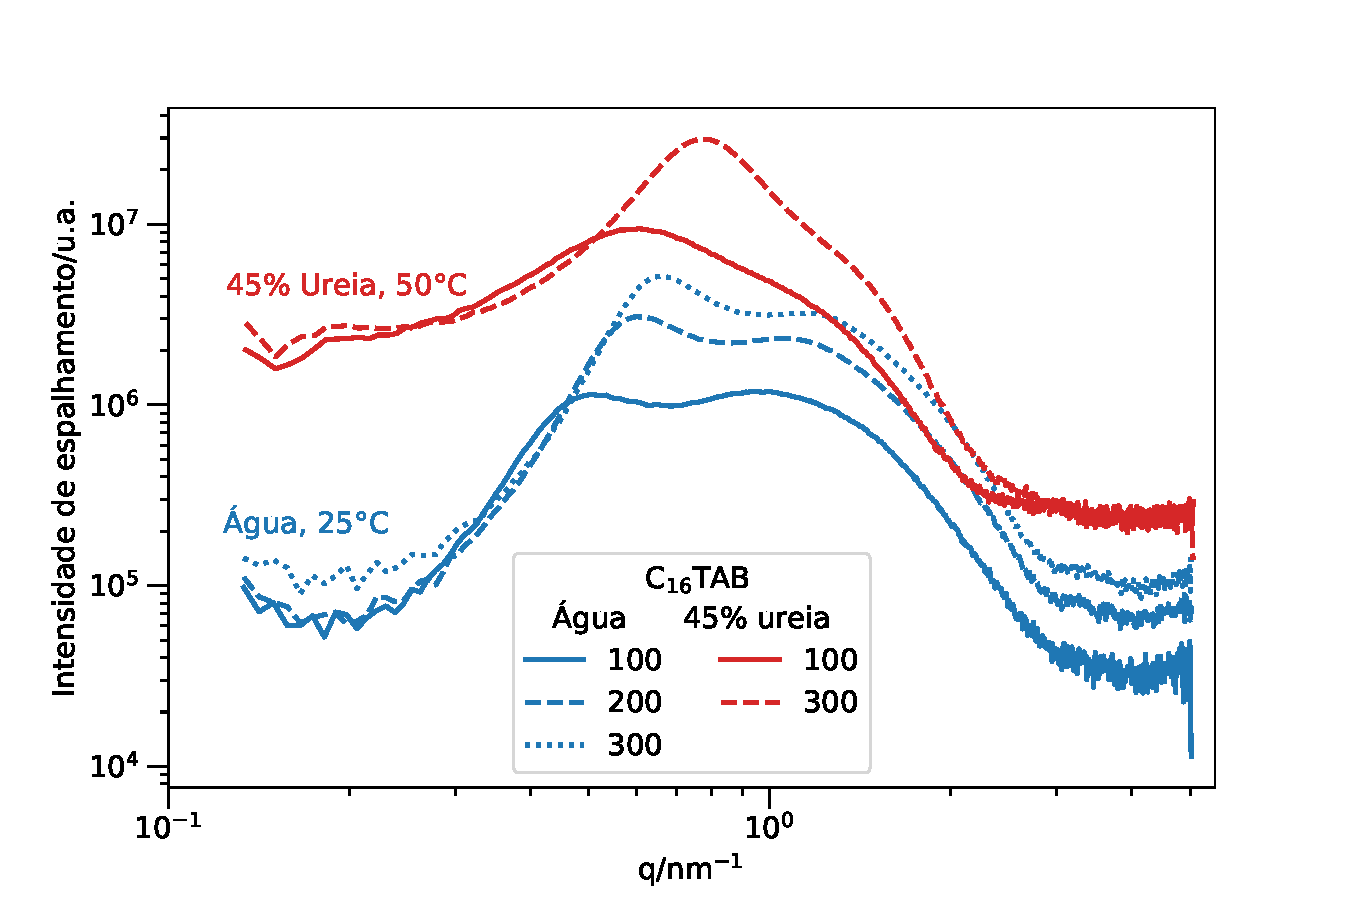
\includegraphics[width=\textwidth]{./imagens/saxs/micelas_CTAB_agua_ureia}
			\caption{\CTAB}
			\label{fig:SAXS_CTAB_com_sem_ureia}
		\end{subfigure} %
		\begin{subfigure}[t]{0.5\textwidth}
			\centering
			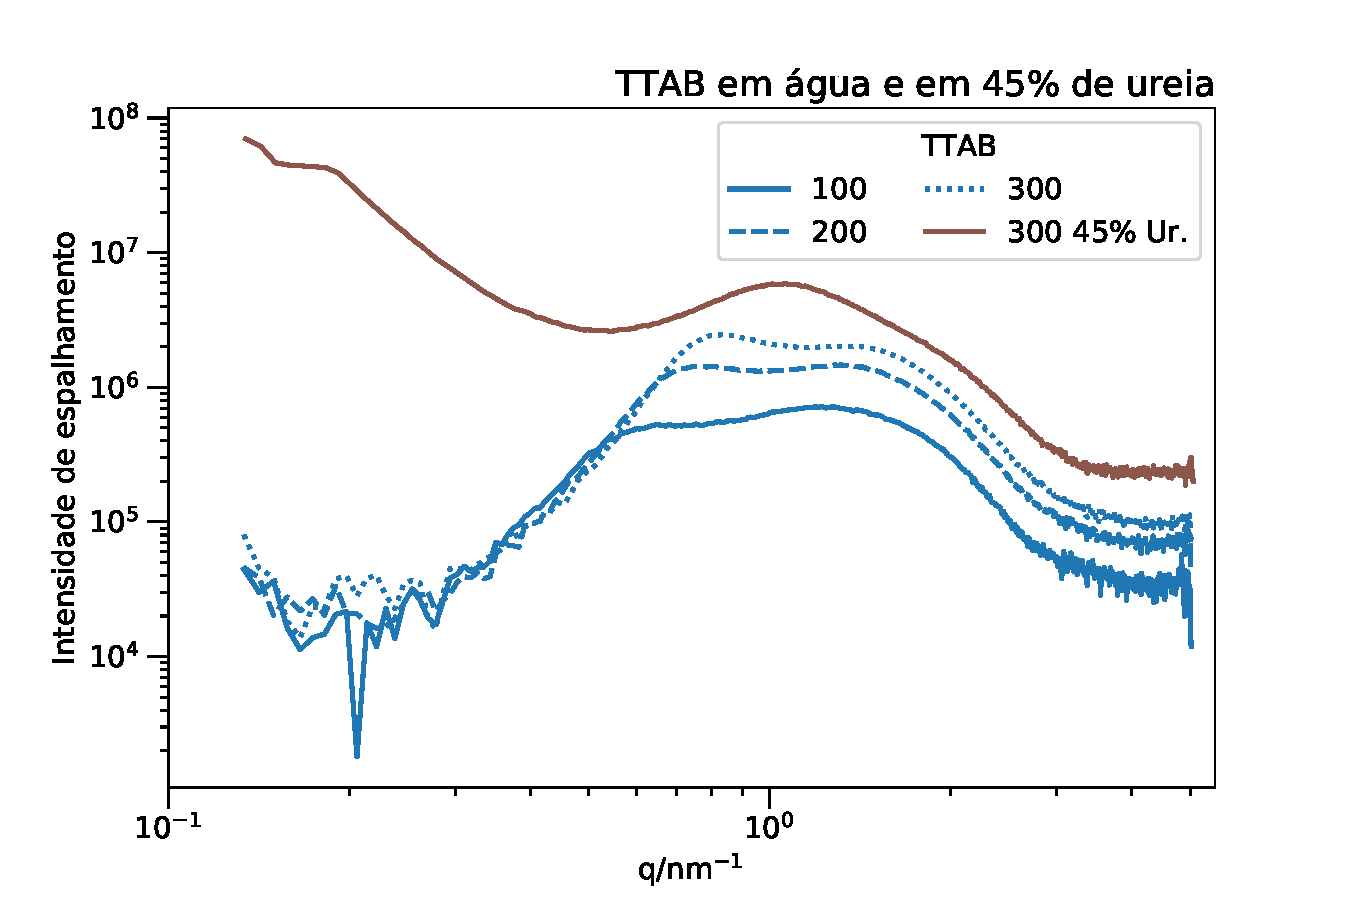
\includegraphics[width=\textwidth]{./imagens/saxs/micelas_TTAB_agua_ureia}
			\caption{\TTAB}
			\label{fig:SAXS_TTAB_com_sem_ureia}
		\end{subfigure}
		\caption{Curvas de SAXS de \CTAB{} (\ref{fig:SAXS_CTAB_com_sem_ureia}) e \TTAB{} (\ref{fig:SAXS_TTAB_com_sem_ureia}) em água a 25°C e em ureia 45\% a 50°C}
		\label{fig:SAXS_com_sem_ureia}
	\end{figure}
	
	Vemos então a grande similaridade das curvas. Há diferenças na intensidade de espalhamento, provavelmente devido à composição diferente das regiões espalhadoras e devido a uma mudança na temperatura. Na região de baixo \q{} da \autoref{fig:SAXS_TTAB_com_sem_ureia} há uma queda que não existe nas outras curvas. Isso pode ser um erro experimental, devido a uma subtração pouco ideal do \emph{background}, ou também pode haver estruturas maiores nessa amostra, possivelmente vesículas. Dessa maneira, há fortes indícios que ao se aquecer a solução, ocorre uma transição lamela---micela esférica.
	
	Na \autoref{sec:Ureia-DLS}, mostra-se que em temperaturas elevadas, há estruturas com um tamanho de aproximadamente 100-300 nm e outras com tamanhos de 3-5 nm. Esses dados foram obtidos por espalhamento dinâmico de luz. Isso reforça a ideia de que há estruturas pequenas, micelares, nessa temperatura.
	 
	De modo a comparar as estruturas lamelares observadas com a estrutura lamelar do surfactante puro, obteve-se as curvas de SAXS dos três surfactantes sólidos. Os padrões de espalhamento para os surfactantes sólidos estão na \autoref{fig:SAXS_surf_sólido}.

	\begin{figure}[h]
		\centering
		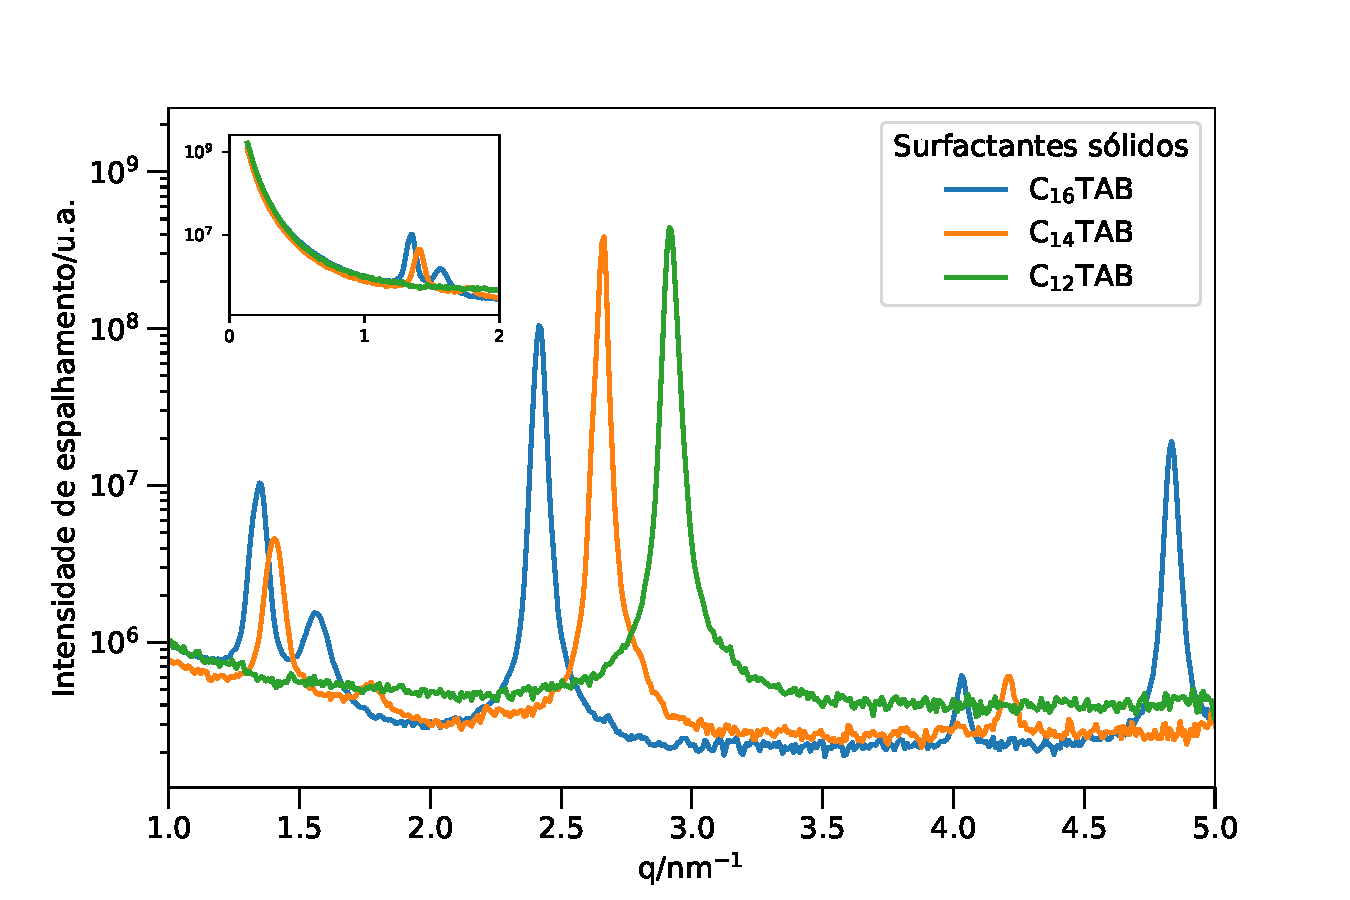
\includegraphics[width=0.7\textwidth]{imagens/saxs/surfactante_solido}
		\caption{Curvas de SAXS de \CTAB{}, \TTAB{} e \DTAB{} sólidos, a 25°C. O \emph{inset} mostra o perfil de espalhamento em valores baixos de \q}
		\label{fig:SAXS_surf_sólido}
	\end{figure} 
	
	Testou-se a indexação das seguintes fases utilizando o programa SGI: H2, Fd3m, Pn3m, Im3m, Pm3n, la3d, P4332, Primitiva, Fm3m e lamelar. Nenhuma dessas fases teve picos coincidentes com os picos mostrados na figura. Portanto, não é possível realizar uma comparação direta com os padrões de espalhamento para as fases lamelares observadas (Figuras \ref{fig:SAXS_ctabconc}, \ref{fig:SAXS_ttabconc}, \ref{fig:SAXS_dtabconc}, \ref{fig:SAXS_ctab300ur37-45}).
	
	Como mostrado na \autoref{sec:teoria_SAXS}, é possível calcular a espessura lamelar \(d_\mathrm{HC}\) a partir da fração volumétrica \(\varphi\) dos componentes. No entanto, não é possível utilizar diretamente a \autoref{eqn:SAXS_frac_volum}, pois é necessário considerar também o outro componente do solvente, a ureia. Por essa razão, foi realizada uma modificação, resultando em
	
	\begin{equation}
		\phi_s = \dfrac{V_{\textit{HC}}\left( \dfrac{w_{s}}{M_{s}} \right)}{\left( V_{\textit{HC}} + V_{P} \right)\dfrac{w_{s}}{M_{s}} + V_{w}\dfrac{w_{w}}{M_{w}} + V_{\textit{ur}}\dfrac{w_{\textit{ur}}}{M_{\textit{ur}}}}
		\label{eqn:SAXS_frac_volum_com_ureia}
	\end{equation} 

	\noindent onde os termos \(V_{\textit{ur}}\), \(w_{\textit{ur}}\) e \(M_{\textit{ur}}\)	se referem ao volume molar parcial de ureia, fração mássica de ureia e massa molar da ureia, respectivamente. Para estimar o comprimento das cadeias, pode-se utilizar a equação de Tanford,\cite{Israelachvili2011}
	
	\begin{equation}
		l = 0{,}150 + 0{,}126n
		\label{eqn:tanford}
	\end{equation}
	
	\noindent onde \(l\) é o comprimento da cadeia de surfactante em nm e \(n\) é o número de carbonos na cadeia. Os volumes das cadeias também podem ser estimadas por uma equação, mas optou-se pelo site \href{www.chemicalize.com}{Chemicalize}\footnote{Acessado em 28/05/2018} para isso. Com isso, foram calculadas as distâncias interlamelares (\autoref{tab:SAXS_distancias_interlamelares}). Foram estimados erros para o máximo dos picos, com base em sua largura e para os volumes para se obter valores de \(d_\mathrm{HC}\) com incerteza. \index{resultados!distâncias interlamelares \(d\)} \index{resultados!espessuras lamelares \(d_\mathrm{HC}\)}
	
		\begin{table}[H]
			\IBGEtab{%
			\caption{Distâncias interlamelares e espessuras lamelares calculadas pelo método de \citeauthor{Ferreira2016}}
			\label{tab:SAXS_distancias_interlamelares}
		}%
		{%
		\begin{tabular}{c c c c c}
			\toprule
			   Surfactante  & Concentração/\mM     & $d$/nm       & \(d_\mathrm{HC}\)/nm & \(l\)/nm               \\ \midrule
			\multirow{3}{*}{\CTAB} & 100              & 36$\pm$5     & 0,9$\pm$0,2          & \multirow{3}{*}{2,16}  \\
			                      & 200              & 23$\pm$1     & 1,1$\pm$0,2          &                        \\
			                      & 300              & 14,6$\pm$0,2 & 1,0$\pm$0,2          &                        \\ \midrule
			\multirow{3}{*}{\TTAB} & 100              & 38$\pm$3     & 0,8$\pm$0,2          & \multirow{3}{*}{1,91}  \\
			                      & 200              & 27$\pm$1     & 1,1$\pm$0,2          &                        \\
			                      & 300              & 13,2$\pm$0,2 & 0,8$\pm$0,1          &                        \\ \midrule
			\multirow{3}{*}{\DTAB} & 100              & 26$\pm$2     & 0,5$\pm$0,1          & \multirow{3}{*}{1,6}   \\
			                      & 200              & 13$\pm$1     & 0,50$\pm$0,08        &                        \\
			                      & 300              & 10,9$\pm$0,3 & 0,58$\pm$0,09        &                        \\ \bottomrule
		\end{tabular}
	}{}
	\end{table} 
	
	Visto que o comprimento da cadeia do surfactante é maior que a espessura lamelar, os valores calculados estão muito longe de serem aceitáveis. Isso ocorreu porque é necessário saber qual é a composição das fases, isto é, quanta água está na fase límpida e quanta água está na fase lamelar. Portanto, é necessário separar a fase lamelar da outra fase, o que pode ser realizado por centrifugação.

	Quanto maior era a concentração de ureia, maior era a resistência das amostras à centrifugação. Além disso, foi necessário utilizar forças de 50000 g (aproximadamente 25000 rpm) para realizar a separação das fases num tempo de horas. Ademais, com velocidades de 5000 rpm, mesmo após sete dias de centrifugação, a separação da amostra não foi completa. As partes superiores foram separadas das partes inferiores, onde estavam as lamelas, e foi feita uma correlação da massa de lamela e a massa do solvente. A partir disso, seria possível calcular a espessura lamelar com a concentração efetiva de surfactante formando a lamela.
	
	Foi realizado um experimento com 35\% (m/m) de ureia de modo a diminuir o tempo de centrifugação. A \autoref{tab:SAXS_centrifug_ur35} mostra as massas obtidas para ambas as fases após a centrifugação de amostras de \CTDTAB{} 100, 200 e 300 \mM{}.
	
	\begin{table}[h]
		\IBGEtab%
		{
			\caption{Massas das fases líquidas \(m_{\text{líquido}}\) e sólidas (lamelas) \(m_{\text{sólido}}\) de amostras de \CTDTAB{} nas concentrações de 100, 200 e 300 \mM{} em 35\% de ureia. \(m_{\text{extra}}\) é a massa de surfactante descontada da fase lamelar.}
			
			\label{tab:SAXS_centrifug_ur35}
		}
		{
			\begin{tabular}{c c | c c c c}
				\toprule
				        Surf.          & \(c_{\text{surf}}\)/\mM & \(m_{\text{líquido}}\)/g & \(m_{\text{sólido}}\)/g & \(m_{\text{surf}}\)/g & \(m_{\text{extra}}\)/g \\ \midrule
				\multirow{3}{*}{\CTAB} & 99,7                    & 2,5251                   & 2,4681                  & 0,1608                & 2,3073                 \\
				                       & 199,2                   & 2,8278                   & 2,1766                  & 0,3118                & 1,8648                 \\
				                       & 299,5                   & 2,9638                   & 2,0391                  & 0,4544                & 1,5847                 \\ \midrule
				\multirow{3}{*}{\TTAB} & 103,6                   & 3,6639                   & 1,3548                  & 0,1551                & 1,1997                 \\
				                       & 199,3                   & 3,6479                   & 1,3523                  & 0,2891                & 1,0632                 \\
				                       & 296,6                   & 3,6396                   & 1,3628                  & 0,4186                & 0,9442                 \\ \midrule
				\multirow{3}{*}{\DTAB} & 97,6                    & 4,5646                   & 0,4443                  & 0,1342                & 0,3101                 \\
				                       & 195,8                   & 4,5670                   & 0,4405                  & 0,2622                & 0,1783                 \\
				                       & 299,9                   & 4,5839                   & 0,4347                  & 0,3916                & 0,0431                 \\ \bottomrule
			\end{tabular}
		}
		{}
	\end{table}
	
	A massa da fase lamelar parece ser independente da concentração de surfactante, isto é, a quantidade de ureia no meio está determinando a concentração da fase lamelar produzida. O \CTAB{} parece ser uma exceção, porém isso pode se dever ao fato de que, mesmo com as velocidades de rotação utilizadas, não foi possível garantir uma separação completa (determinado visualmente). Além disso, observou-se que com o resfriamento da solução de 3°C (para 17°C), ocorreu a formação de mais fase branca, com cristais mais aciculares, visualmente diferente da fase compacta formada após a centrifugação. Possivelmente, há uma proporção entre surfactante e ureia que está compondo a fase límpida. Dessa maneira, não é possível calcular \(d_\mathrm{HC}\) com precisão, pois não foi possível quantificar a concentração das espécies. 
	\FloatBarrier
\section{DLS}
\label{sec:Ureia-DLS}
\index{resultados!DLS}

	De modo a obter informações complementares sobre as soluções em temperaturas elevadas, foram realizadas medidas de DLS de amostras de \CTTAB{} 100, 200, 300 \mM{} e 40\% (m/m) de ureia a 50°C. \DTAB{} não foi analisado por possuir essencialmente os mesmos padrões dos outros surfactantes. As distribuições de tamanho (Figuras \ref{fig:DLS_ctab_distrib}, \ref{fig:DLS_ttab_distrib}), obtidas a partir de um ajuste das curvas de correlação (Figuras \ref{fig:DLS_ctab_cc}, \ref{fig:DLS_ttab_cc}). Cada medida foi feita em triplicata.
	

\begin{figure}[h]
	\begin{subfigure}{0.50\textwidth}
		\centering
		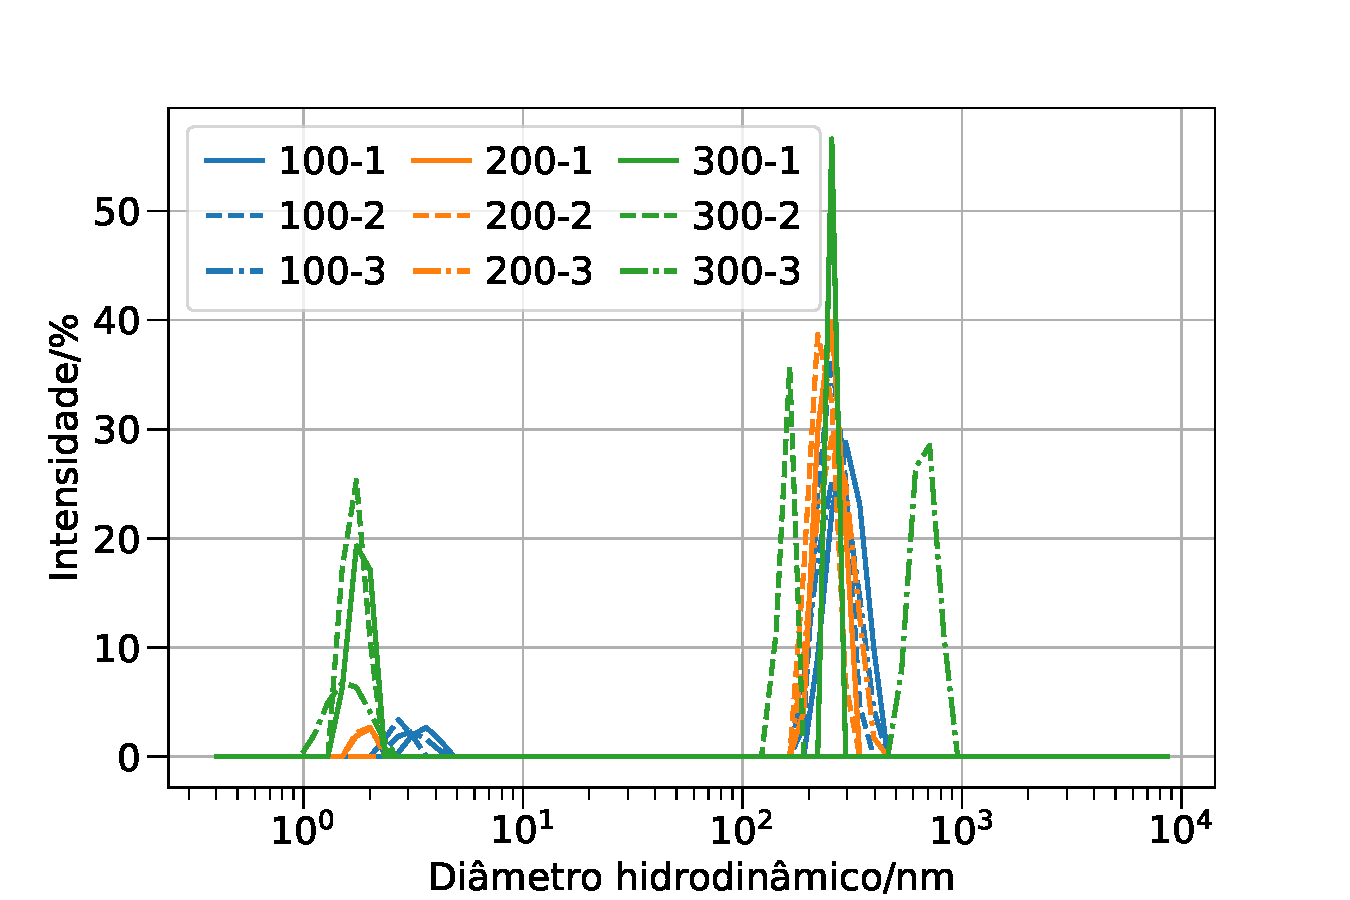
\includegraphics[width=\textwidth]{imagens/dls/ctab_distrib}
		\caption{Distribuições de raio hidrodinâmico}
		\label{fig:DLS_ctab_distrib}
	\end{subfigure} %
	\begin{subfigure}{0.50\textwidth}
		\centering
		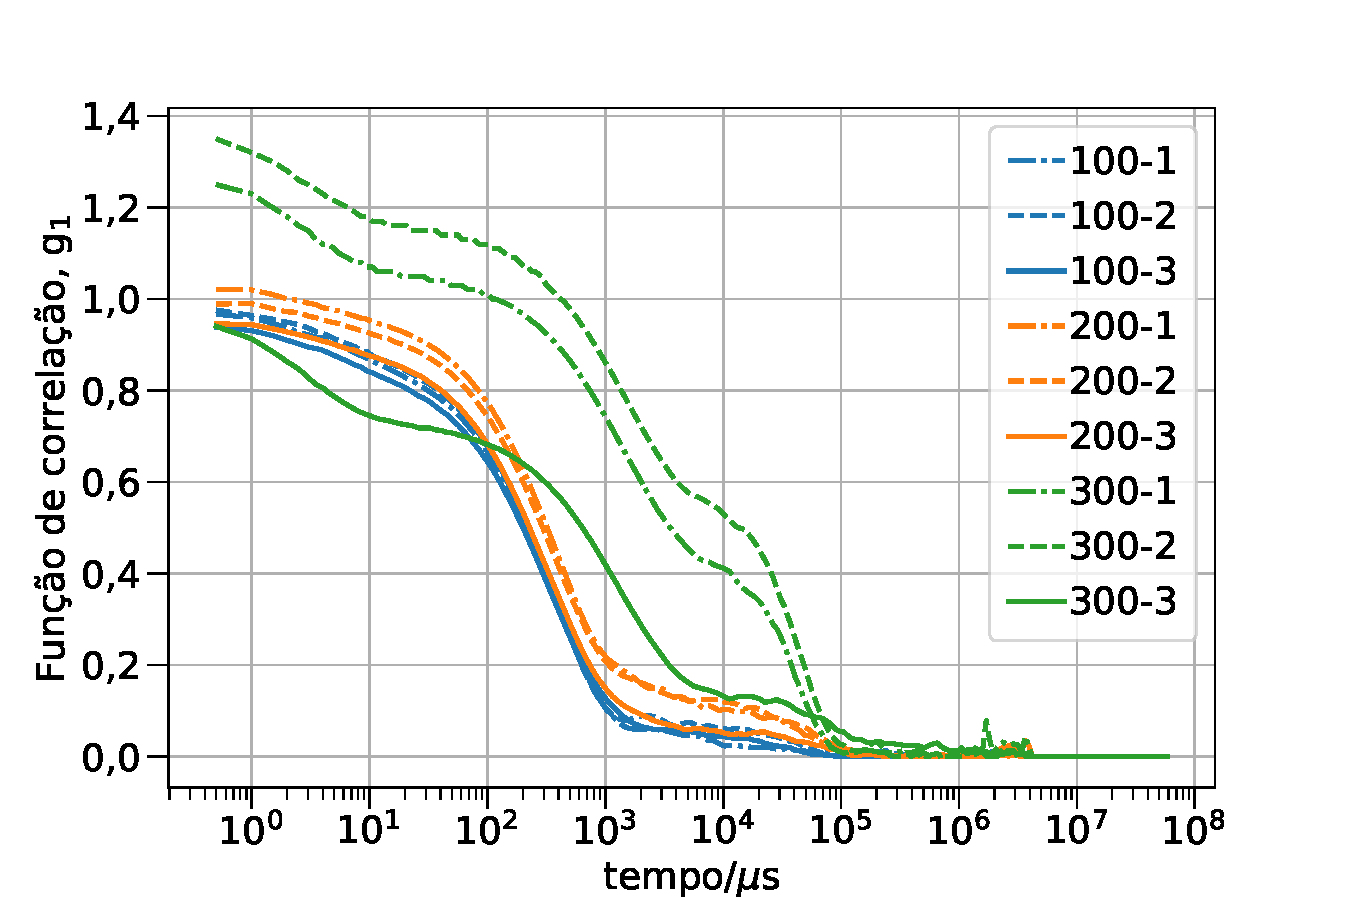
\includegraphics[width=\textwidth]{imagens/dls/ctab_CC}
		\caption{Curvas de correlação}
		\label{fig:DLS_ctab_cc}
	\end{subfigure}
	\caption{Curvas de distribuição de tamanho e de correlação de \CTAB{} 100, 200 e 300 \mM{} com 40\% de ureia a 50°C, obtidos em triplicatas}
	\label{fig:DLS_ctab}
\end{figure}

%% Distribuições e CC de TTAB
\begin{figure}[h]
	\begin{subfigure}{0.50\textwidth}
		\centering
		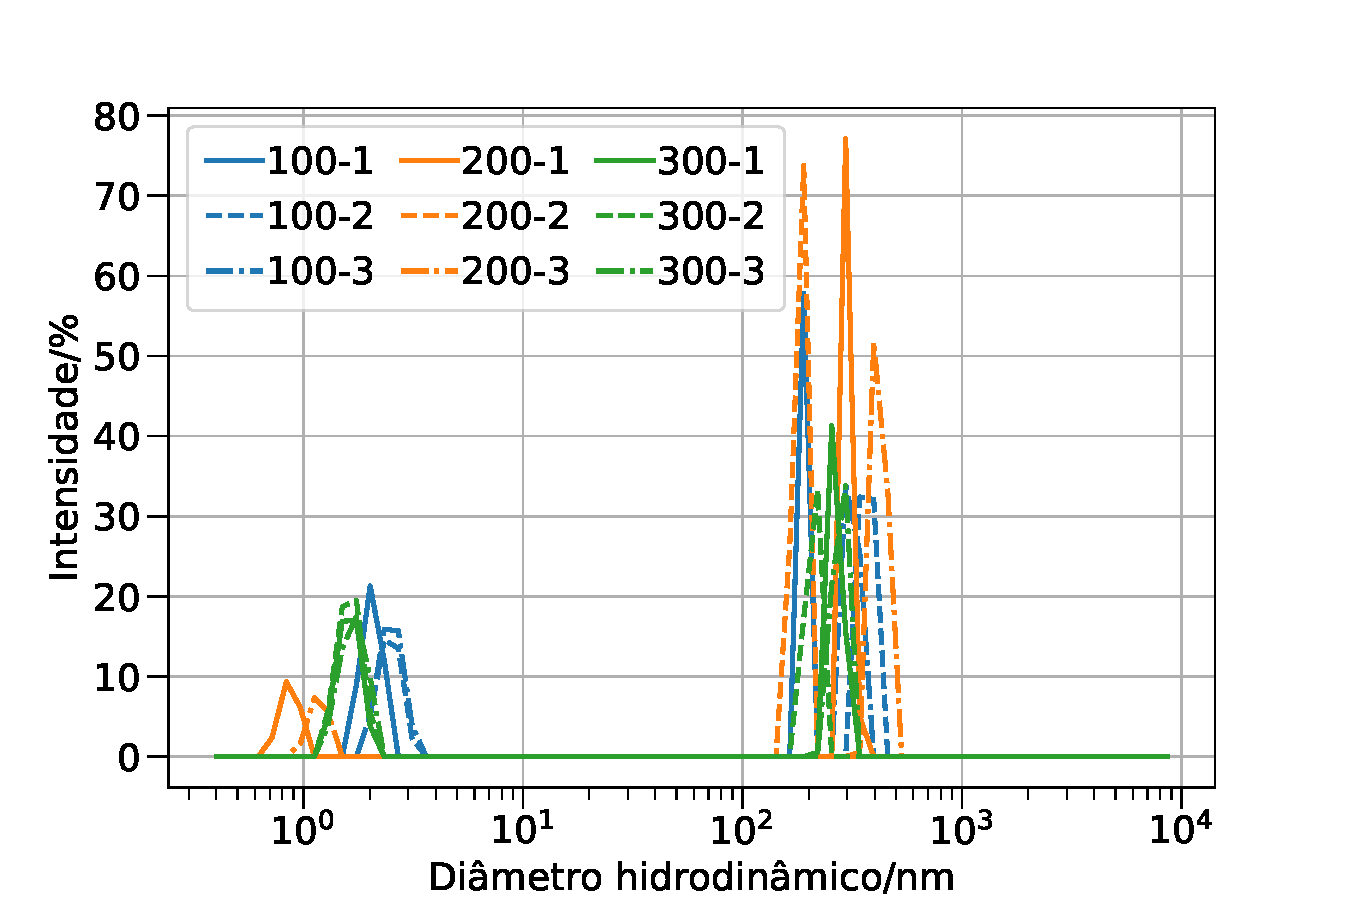
\includegraphics[width=\textwidth]{imagens/dls/ttab_distrib}
		\caption{Distribuições de raio hidrodinâmico}
		\label{fig:DLS_ttab_distrib}
	\end{subfigure} %
	\begin{subfigure}{0.50\textwidth}
		\centering
		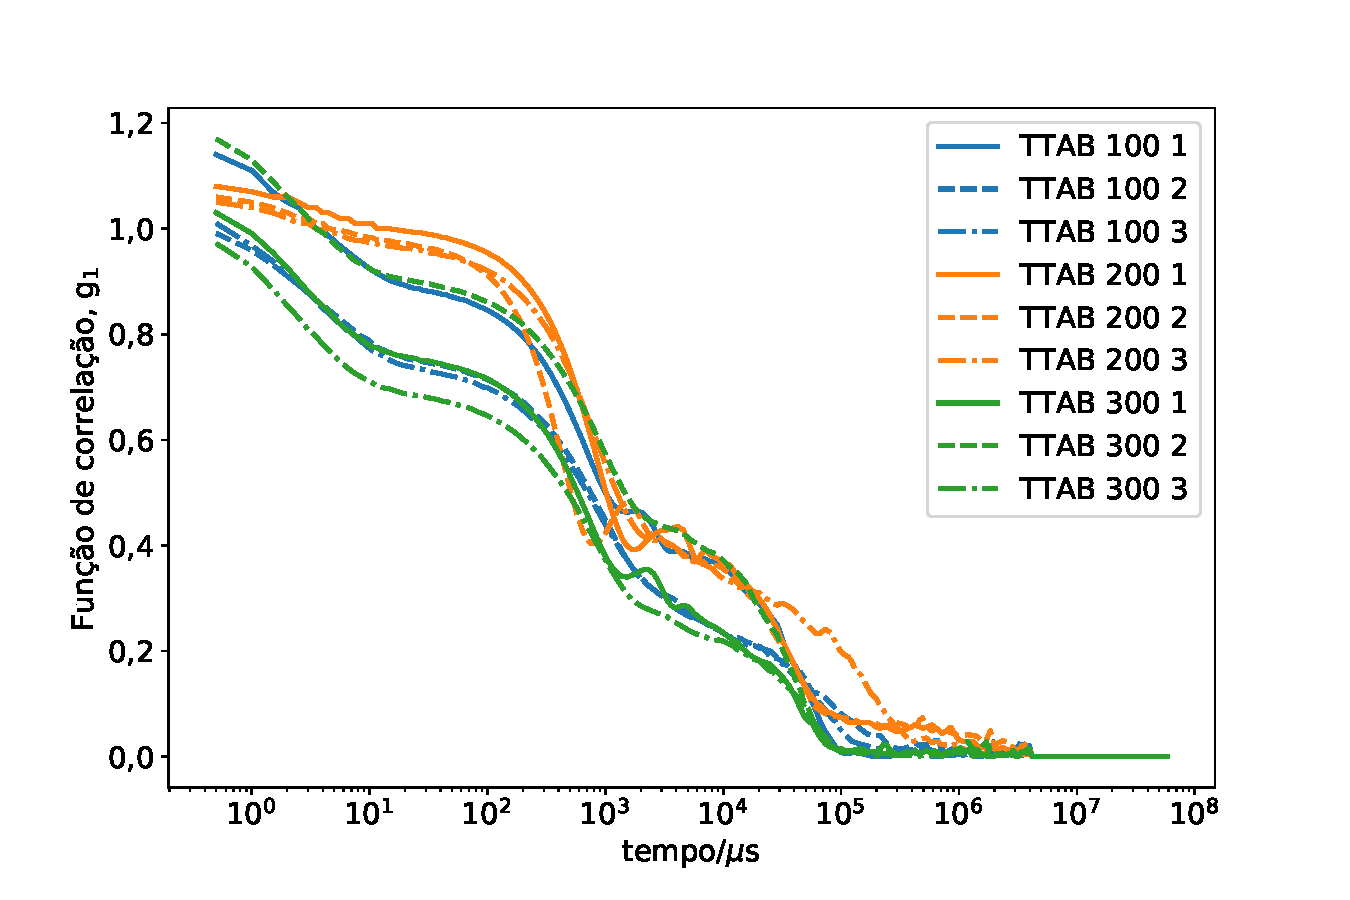
\includegraphics[width=\textwidth]{imagens/dls/ttab_CC}
		\caption{Curvas de correlação}
		\label{fig:DLS_ttab_cc}
	\end{subfigure}
	\caption{Curvas de distribuição de tamanho e de correlação de \TTAB{} 100, 200 e 300 \mM{} com 40\% de ureia a 50°C, obtidos em triplicatas}
	\label{fig:DLS_ttab}
\end{figure}

%	As Figuras \ref{fig:DLS_distrib_conc} e \ref{fig:DLS_CC_conc} comparam as distribuições de tamanho e curvas de correlação, respectivamente, para amostras com concentrações iguais de surfactante, \CTAB{} ou \TTAB.

%\begin{figure}[h]
%	\begin{subfigure}{0.3\textwidth}
%		\centering
%		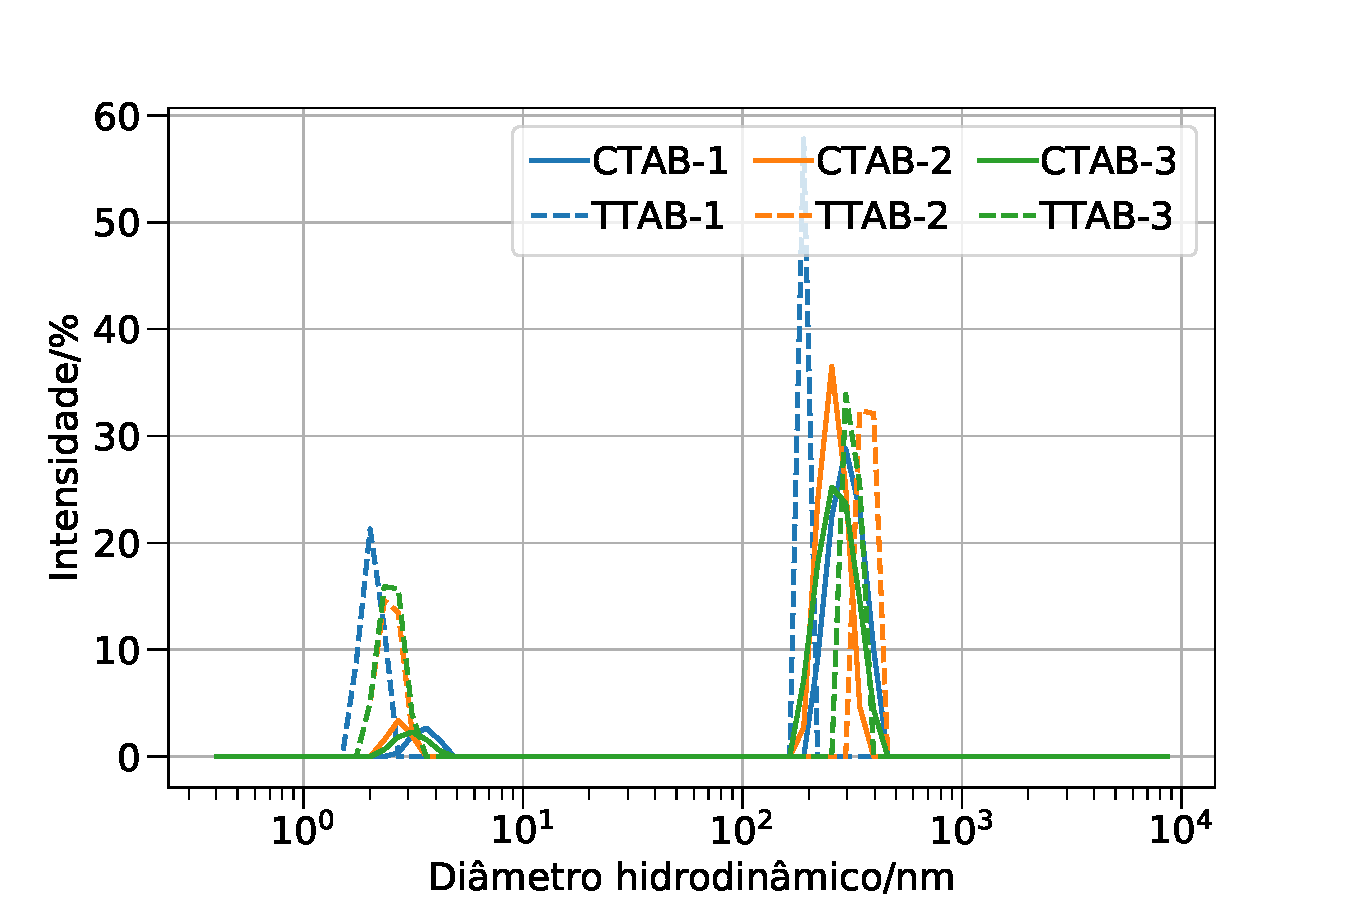
\includegraphics[width=\textwidth]{imagens/dls/100_distrib}
%		\caption{100\mM}
%		\label{fig:DLS_100_distrib}
%	\end{subfigure} %
%	\begin{subfigure}{0.3\textwidth}
%		\centering
%		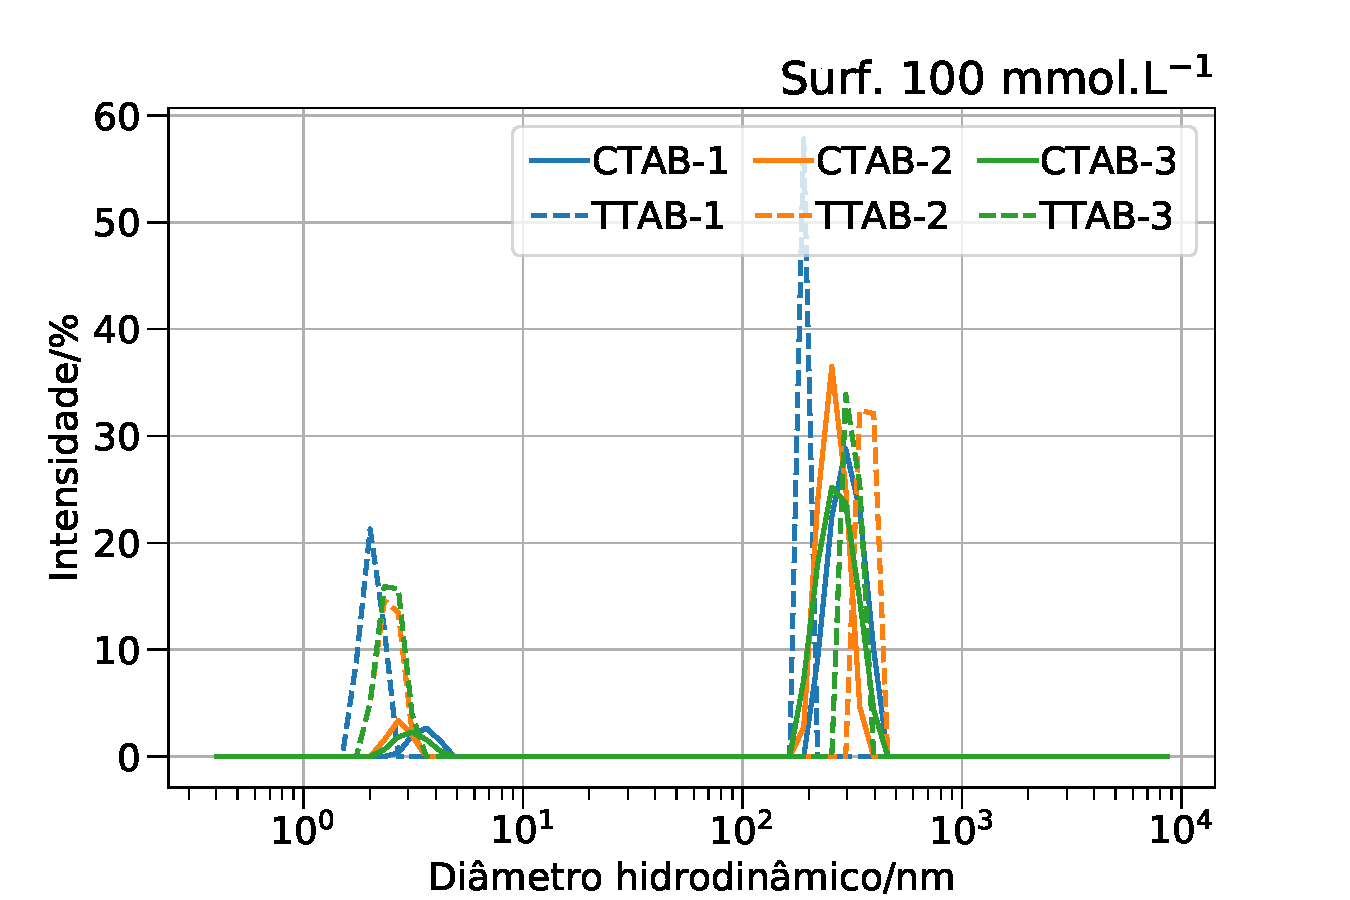
\includegraphics[width=\textwidth]{imagens/dls/200_distrib}
%		\caption{200\mM}
%		\label{fig:DLS_200_distrib}
%		\end{subfigure} %
%	\begin{subfigure}{0.3\textwidth}
%		\centering
%		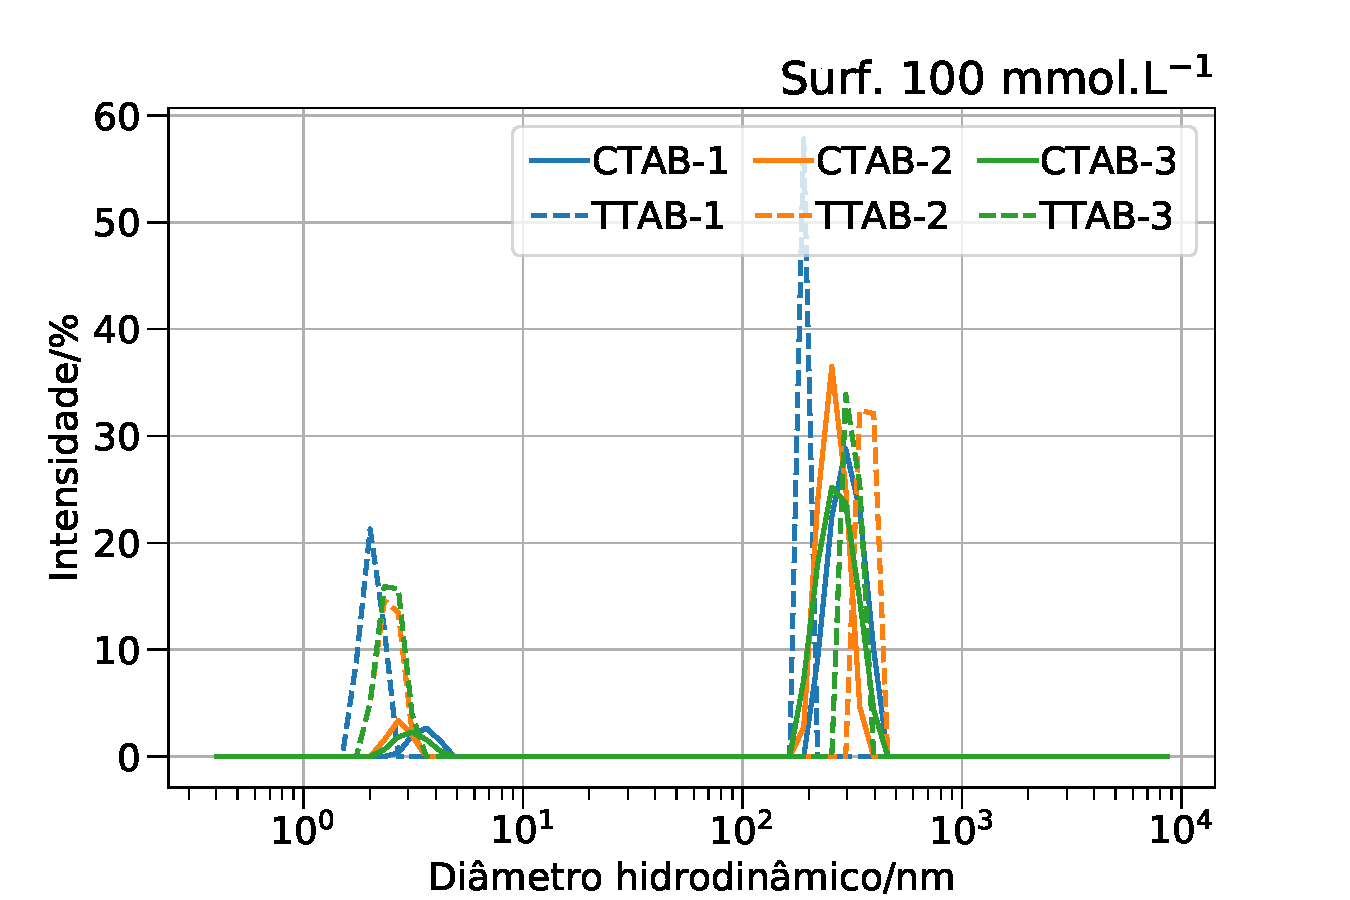
\includegraphics[width=\textwidth]{imagens/dls/300_distrib}
%		\caption{300\mM}
%		\label{fig:DLS_300_distrib}
%	\end{subfigure}
%	\caption{Curvas de distribuição de tamanhos de \CTTAB{} 100, 200 e 300 \mM{} e 40\% (m/m) de ureia a 50°C}
%	\label{fig:DLS_distrib_conc}
%\end{figure}

%\begin{figure}[h]
%	\begin{subfigure}{0.3\textwidth}
%		\centering
%		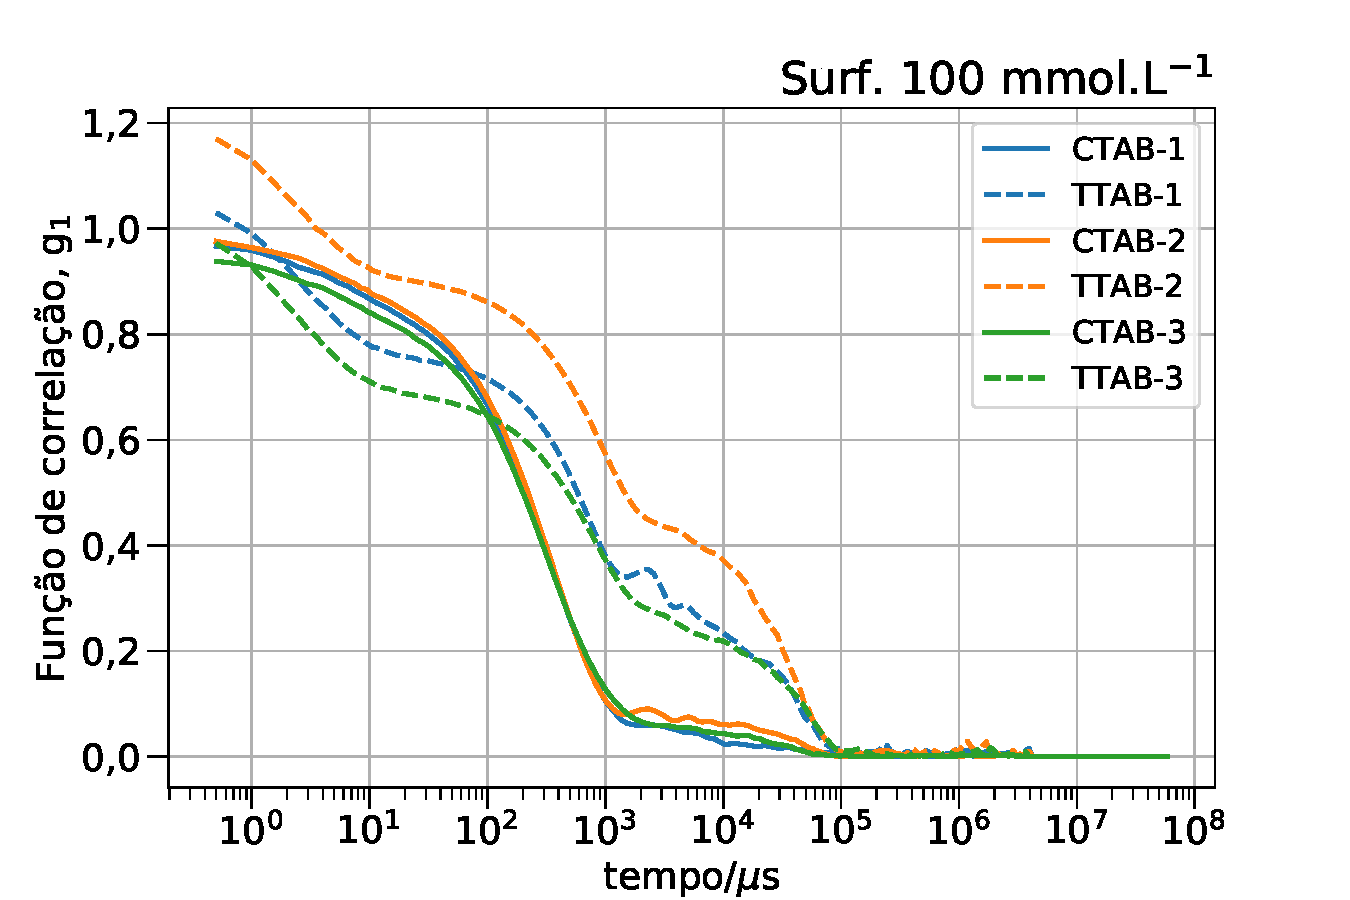
\includegraphics[width=\textwidth]{imagens/dls/100_CC}
%		\caption{100 \mM}
%		\label{fig:DLS_100_CC}
%	\end{subfigure} %
%	\begin{subfigure}{0.3\textwidth}
%		\centering
%		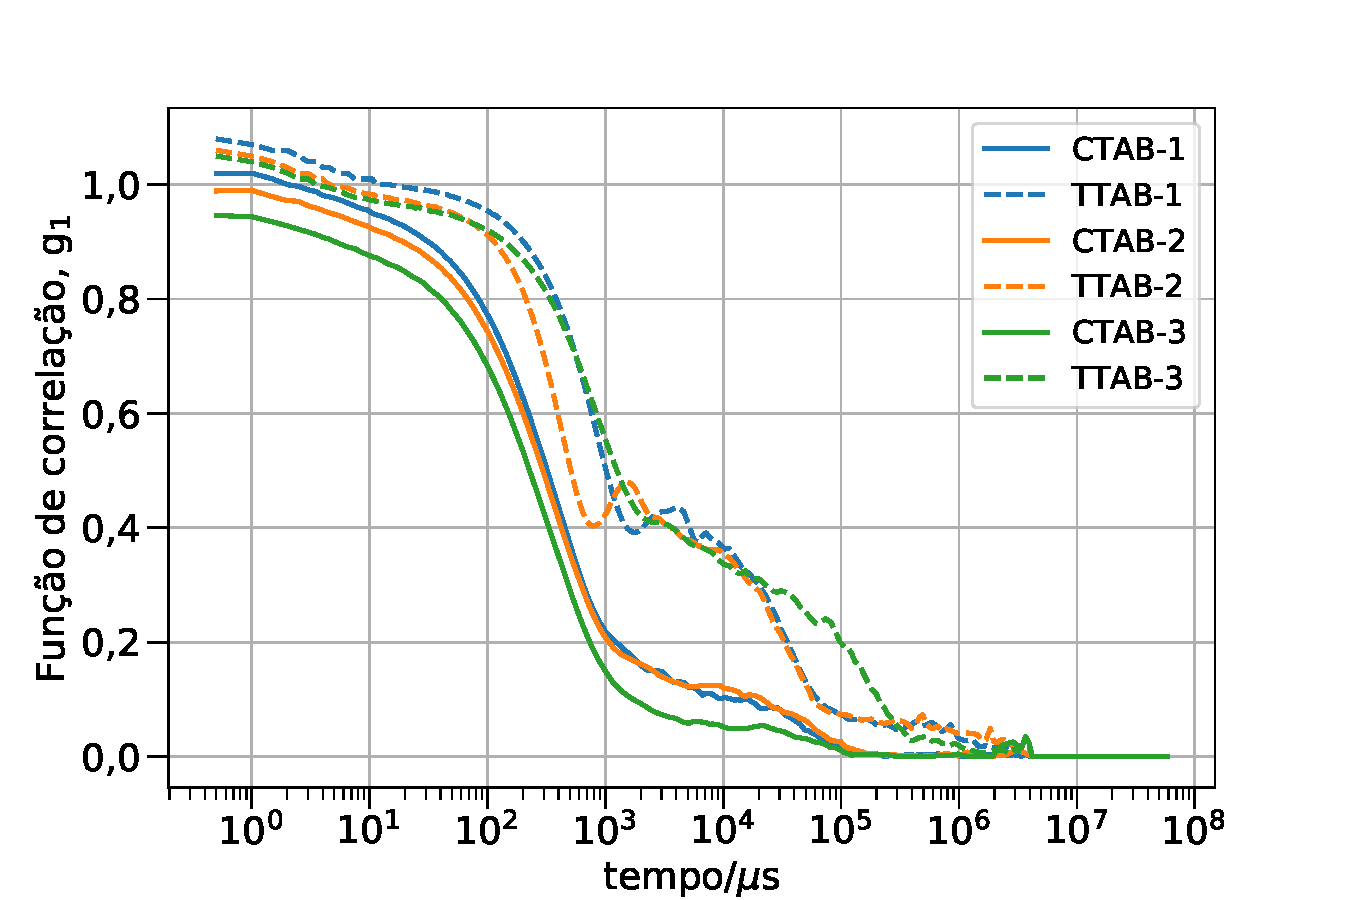
\includegraphics[width=\textwidth]{imagens/dls/200_CC}
%		\caption{200 \mM}
%		\label{fig:DLS_200_CC}
%	\end{subfigure} %
%	\begin{subfigure}{0.3\textwidth}
%		\centering
%		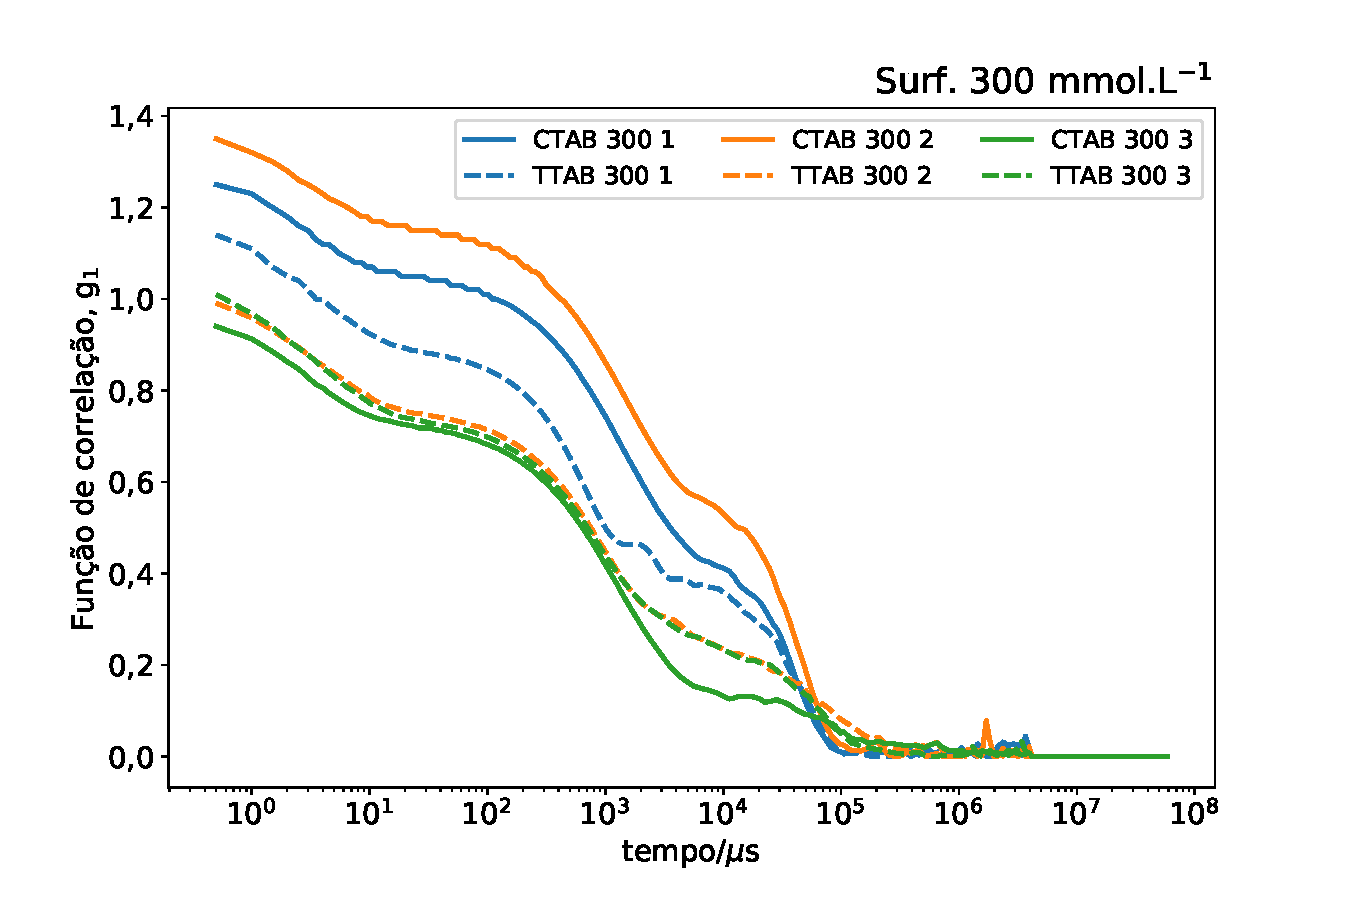
\includegraphics[width=\textwidth]{imagens/dls/300_CC}
%		\caption{300 \mM}
%		\label{fig:DLS_300_CC}
%	\end{subfigure}
%	\caption{Curvas de correlação de \CTTAB 100, 200 e 300 \mM{} a 50°C}
%	\label{fig:DLS_CC_conc}
%\end{figure}

	Pode-se observar que não há diferenças muito significativas entre as amostras, tanto se comparadas concentrações diferentes quanto surfactantes diferentes. Nota-se que há estruturas pequenas, na faixa de 3-5 nm de diâmetro, muito provavelmente micelas esféricas, como visto anteriormente por SAXS. Além disso, há estruturas com tamanhos de 100 a 300 nm. Devido à baixa viscosidade e transparência das soluções, é possível que existam lamelas em forma de vesículas nessas condições, em conjunto com micelas esféricas.
	
	A qualidade das curvas de correlação é muito ruim, havendo muitas irregularidades, como valores de \(g_1\) maiores que 1, e vários perfis de decaimento sobrepostos, indicativos de várias estruturas com raios diferentes. No entanto, juntando as informações obtidas por SAXS e por DLS, é possível concluir, com relativa certeza, de que acima da temperatura de transição, são formadas micelas esféricas. 
	
%%% Imagens DTAB %%%%%%%%%%%%%%%%%%%%%%%%%%%%%%%%%%%%%%%%%%%%%%%%%%%%%%%%%%%%%%
%\begin{figure}[H]
%	\begin{subfigure}{0.47\textwidth}
%		\centering
%		\includegraphics[width=\textwidth]{imagens/dls/dtab_distrib}
%		\caption{Distribuições de raio hidrodinâmico}
%		\label{fig:DLS_dtab_distrib}
%	\end{subfigure} \qquad %
%	\begin{subfigure}{0.47\textwidth}
%		\centering
%		\includegraphics[width=\textwidth]{imagens/dls/dtab_CC}
%		\caption{Curvas de correlação}
%		\label{fig:DLS_dtab_cc}
%	\end{subfigure}
%	\caption{DLS de DTAB 200 \mM{} a 50°C}
%	\label{fig:DLS_dtab}
%\end{figure}
%%%%%%%%%%%%%%%%%%%%%%%%%%%%%%%%%%%%%%%%%%%%%%%%%%%%%%%%%%%%%%%%%%%%%%%%%%%%%%%%%

% todo: pensar se eu devo colocar dados sobre reologia, já que tem somente dados com salicilato, e se eu devo fazer mais experimentos com o sólido sozinho.

%\section{Reologia do sólido}
%
%Amostras de ureia abaixo da temperatura de transição foram analisadas no reômetro e os resultados estão na Figura. X
\FloatBarrier
\section{Entalpia de interação de ureia com surfactante} \index{resultados!ITC}

	De modo a investigar a espontaneidade da interação entre ureia e micelas de \TTAB{}, foram realizadas titulações calorimétricas isotérmicas de ureia sobre uma solução de \TTAB{} 12 \mM, e foi descontado o valor da titulação de ureia em água. Utilizou-se concentrações crescentes de ureia, de 40 a 160 \mM. Não foi possível testar concentrações maiores de ureia, semelhantes às condições experimentais das seções anteriores, porque o calor de interação se tornava muito intenso. A \autoref{fig:itc_interacaoUrSurf_entalpograma} mostra os entalpogramas com o branco já descontado, obtidos em função da concentração de ureia na cela. Foram realizados ajustes lineares  dessas curvas para se obter o valor do intercepto quando a concentração de ureia tende a zero. Os valores estão na \autoref{fig:itc_interacaoUrSurf_intercepto}.
	
	%É possível exibir este gráfico em função do número da titulação ou da concentração de TTAB na cela, porém a maneira apresentada se mostra mais relevante.
	% todo: colocar o snippet que tratou isso.

\begin{figure}[h]
	\centering
	\includegraphics[width=0.7\textwidth]{imagens/itc/interacao_ureia_surf}
	\caption{Entalpogramas da titulação de ureia em \TTAB{} 12\mM, com o calor normalizado pela concentração de surfactante na cela e com subtração do branco. As linhas contínuas são ajustes lineares.}
	\label{fig:itc_interacaoUrSurf_entalpograma}
\end{figure}


\begin{figure}[h]
	\centering
	\includegraphics[width=0.7\textwidth]{imagens/itc/interacao_intercepto}
	\caption{Entalpia de interação de ureia/surfactante em função da concentração de ureia utilizada na titulação, obtidos pelo intercepto dos ajustes lineares.}
	\label{fig:itc_interacaoUrSurf_intercepto}
\end{figure}

	Podemos observar que os valores para as concentrações menores de ureia são iguais entre si, cerca de 7.8 J por mol de surfactante na cela. Somente quando a concentração se torna muito alta, o valor de interação diminui. Esse valor é bastante pequeno, indicando que a interação de ureia com o grupo trimetilamônio, nessas condições, é pouco intensa. Para comparação, a \autoref{fig:itc_interacaoUrAgua} mostra os brancos de titulação de ureia em água. Observamos que esses valores são maiores que os valores calculados para a interação surfactante-ureia.
	
	% todo: esses calores são endotérmicos. Qual seria a explicação? São assim melhores? Não seria melhor algo o quanto mais negativo possível?
	% todo: pensar se vale a pena colocar os RAW ITCs para mostrar que os dados foram bem adquiridos.

\begin{figure}[h]
	\centering
	\includegraphics[width=0.7\textwidth]{imagens/itc/interacao_branco}
	\caption{Entalpogramas da titulação de ureia em água}
	\label{fig:itc_interacaoUrAgua}
\end{figure}
	
	 Para facilitar a comparação, a \autoref{fig:itc_comparativo_tit_ureia_agua_ureia_ttab} mostra os calores registrados pelo equipamento tanto na titulação de ureia em água quanto na titulação de ureia em \TTAB{} 12 \mM. 
	 
\begin{figure}[h]
	\begin{subfigure}{0.5\textwidth}
		\centering
		\includegraphics[width=\textwidth]{imagens/itc/interacao_ureia_surf_dq}
		\caption{Titulação ureia em \TTAB{} 12 \mM{} com subtração do branco}
		\label{fig:itc_interacaoUreiaSurfDq}
	\end{subfigure} %
	\begin{subfigure}{0.5\textwidth}
		\centering
		\includegraphics[width=\textwidth]{imagens/itc/interacao_branco_dq}
		\caption{Titulação ureia em água}
		\label{fig:itc_interacaoUreiaAguaDq}
	\end{subfigure} 

	\caption{Calores experimentais sem normalização para as titulações de ureia em água e em solução de \TTAB{} 12 \mM. A a \autoref{fig:itc_interacaoUreiaSurfDq} faz paralelo com a \autoref{fig:itc_interacaoUrSurf_entalpograma} e a \autoref{fig:itc_interacaoUreiaAguaDq} faz paralelo com a \autoref{fig:itc_interacaoUrAgua}. As retas representam a tendência de cada curva, obtidas através de um ajuste linear.}
	\label{fig:itc_comparativo_tit_ureia_agua_ureia_ttab}
\end{figure}
	
	Há uma notável semelhança entre as curvas da \autoref{fig:itc_interacaoUreiaAguaDq} e \autoref{fig:itc_interacaoUrAgua}, com primariamente um deslocamento nos valores absolutos das curvas, pois não houve a normalização pela concentração de espécie na cela. Já a \autoref{fig:itc_interacaoUreiaSurfDq} difere grandemente da \autoref{fig:itc_interacaoUrSurf_entalpograma} principalmente porque a concentração de \TTAB{} diminui no decorrer da titulação, então o valor de \(\Delta H/J.mol^{-1} \text{de surfactante na cela}\) difere de \(\Delta q/J\). Vemos o mesmo padrão, com as curvas de 40, 80 e 120 \mM{} de ureia na seringa partindo do mesmo ponto e a curva de 160 \mM{} de ureia na seringa paralela à curva de 120 \mM.
	
	A entalpia de dissolução de ureia em água é positiva, como foi observado durante a mistura dos componentes durante o preparo de amostra. Logo, é razoável que a entalpia de diluição de ureia também seja, pois interações ureia-ureia e ureia-água estão sendo trocadas por interações ureia-água e água-água, respectivamente.
	
	Foi levantada também a hipótese de que a ureia está aumentando a concentração micelar crítica do surfactante, levando à sua desmicelização durante a titulação com \TTAB{}. Porém, o aumento da CMC somente ocorre de maneira apreciável em concentrações muito maiores de ureia, então os efeitos observados devem ser somente devido à interação de micelas de \TTAB{} com ureia.
	
	O código utilizado para gerar a \autoref{fig:itc_interacaoUrSurf_entalpograma} se encontra nas listagens \ref{lst:codigo_itc_ureia} e \ref{lst:codigo_itc_ureia2}. As outras figuras foram geradas com códigos semelhantes, alterando-se os valores de y.
	
	\begin{listing}[h]
		\inputminted{python}{./python/ITC_tratamento_ureia_ttab.py}
		\caption{Código utilizado para gerar a \autoref{fig:itc_interacaoUrSurf_entalpograma} (1/2)}
		\label{lst:codigo_itc_ureia}
	\end{listing}

	\begin{listing}[h]
		\inputminted{python}{./python/ITC_tratamento_ureia_ttab2.py}
		\caption{Código utilizado para gerar a \autoref{fig:itc_interacaoUrSurf_entalpograma} (1/2)}
		\label{lst:codigo_itc_ureia2}
	\end{listing}


	\FloatBarrier
	
	\section{Conclusão} \index{conclusões!ureia}
	
	A ureia demonstrou possuir um comportamento muito diferente dos outros aditivos estudados. Ocorre a formação de fases lamelares com temperaturas de transição entre 20 e 40°C, dependendo da concentração de ureia, e do comprimento da cadeia do surfactante. Essa fase lamelar se separa da outra fase, que é límpida e fluida, mas somente após forte centrifugação. A formação das lamelas é fundamentalmente regida pela ureia, pois a adição de mais surfactante não levou à sua incorporação na fase lamelar, já que era possível precipitar o excesso de surfactante com o abaixamento da temperatura. Em temperaturas acima da temperatura de transição, a fase lamelar se transformava numa fase límpida e pouco viscosa, semelhante à outra fase em temperaturas baixas, que contém principalmente micelas esféricas, mas possivelmente contém vesículas. Com isso, a fase lamelar foi caracterizada com a clareza necessária para este trabalho.
	
	Como próximos estudos, seria interessante obter um diagrama de fase completo de surfactante e ureia, e determinar a concentração de ureia, e de surfactante, em ambas as fases. Assim, seria mais fácil propor um modelo para as estruturas formadas, qual seria o papel da ureia na formação dos agregados, e porque ocorre a separação de fases.
	
	